\documentclass[twoside,english]{uiofysmaster}


\usepackage{simpler-wick}
\usepackage{mathtools}
\usepackage{amsmath}
\usepackage{tabularx}
\usepackage{graphicx}
\usepackage{flexisym}
\usepackage{listings}
\usepackage[most]{tcolorbox}
\usepackage{xcolor}
\usepackage{hyperref}
\usepackage{amsthm}
\usepackage{subcaption}
\usepackage{lscape}
\usepackage[toc,title,page]{appendix}
\usepackage{cancel}
\usepackage[backend=bibtex]{biblatex}
\addbibresource{master.bib}
\usepackage[linesnumbered,lined,boxed,commentsnumbered,ruled]{algorithm2e}
\usepackage{tikz}
%
% \usepackage{tikz}
\usetikzlibrary{calc}
\usetikzlibrary{decorations.pathreplacing,decorations.markings}

%from tex.stackexchange.com
\tikzset{
  % style to apply some styles to each segment of a path
  on each segment/.style={
    decorate,
    decoration={
      show path construction,
      moveto code={},
      lineto code={
        \path [#1]
        (\tikzinputsegmentfirst) -- (\tikzinputsegmentlast);
      },
      curveto code={
        \path [#1] (\tikzinputsegmentfirst)
        .. controls
        (\tikzinputsegmentsupporta) and (\tikzinputsegmentsupportb)
        ..
        (\tikzinputsegmentlast);
      },
      closepath code={
        \path [#1]
        (\tikzinputsegmentfirst) -- (\tikzinputsegmentlast);
      },
    },
  },
  % style to add an arrow in the middle of a path
  mid arrow/.style={postaction={decorate,decoration={
        markings,
  %                     place for arrows
        mark=at position .62 with {\arrow[#1]{>}}
      }}},
  % style to add an arrow in the middle of a path
  mid rarrow/.style={postaction={decorate,decoration={
        markings,
  %                     place for arrows
        mark=at position .38 with {\arrow[#1]{<}}
      }}},
  % style to add a double-headed arrow in the middle of a path
  mid darrow/.style={postaction={decorate,decoration={
        markings,
  %                     place for arrows
        mark=at position .62 with {\arrow[#1]{>>}}
      }}},
  % style to add a double-headed arrow in the middle of a path
  mid rdarrow/.style={postaction={decorate,decoration={
        markings,
  %                     place for arrows
        mark=at position .38 with {\arrow[#1]{<<}}
      }}},
}

% from http://tex.stackexchange.com/questions/25678/nicer-wavy-line-with-tikz
\pgfdeclaredecoration{complete sines}{initial}
{
  \state{initial}[
        width=+0pt,
        next state=sine,
        persistent precomputation={\pgfmathsetmacro\matchinglength{
            \pgfdecoratedinputsegmentlength / int(\pgfdecoratedinputsegmentlength/\pgfdecorationsegmentlength)}
            \setlength{\pgfdecorationsegmentlength}{\matchinglength pt}
        }] {}
  \state{sine}[width=\pgfdecorationsegmentlength]{
        \pgfpathsine{\pgfpoint{0.25\pgfdecorationsegmentlength}{0.5\pgfdecorationsegmentamplitude}}
        \pgfpathcosine{\pgfpoint{0.25\pgfdecorationsegmentlength}{-0.5\pgfdecorationsegmentamplitude}}
        \pgfpathsine{\pgfpoint{0.25\pgfdecorationsegmentlength}{-0.5\pgfdecorationsegmentamplitude}}
        \pgfpathcosine{\pgfpoint{0.25\pgfdecorationsegmentlength}{0.5\pgfdecorationsegmentamplitude}}
  }
  \state{final}{}
}

%
%             CCDiag v.1.0 
%           D.Kats, September 2011
%
% \bdiag[<scale>] start diagram. If <scale> is given, the diagram will be scaled
% \bdiags[<scale>]: the H diagram will be placed in the middle (otherwise it is shifted halfway to the vacuum)
%
% \dT[<order>]{<exc.level>}{<node>} -> T_<exc.level>^{(<order>)}
% node-names are generated as <node>1, <node>2, <node>3, ...
% can be used without <order> (\dT{<exc.level>}{<node>})
% same with \dU (will print U_<exc.level> as label)
% for excitation operators without label use \dTs
% One can customize labels (see e.g. how \dU is defined)
% \dTd, \dTds, \dUd are T^{\dagger}, {}^{\dagger}, U^{\dagger}
%
% \dTdv[<order>]{<exc.level>}{<node>} : draw vacuum explicitly (\tau^\dagger) 
% \dTv[<order>]{<exc.level>}{<node>} -> \tau
%
% \dF{<node>} -> F
% \dFs{<node>} : one-electron operator without label
% \dX{<node>} : one-electron perturbation (X as label)
% \dHone[<name>]{<node>} : one-electron operator with label <name> 
% \dW{<left node>}{<right node>} -> W
% \dWs{<left node>}{<right node>} : two-electron operator without label
% \dXtwo{<left node>}{<right node>} : two-electron perturbation (X as label)
% \dHtwo[<name>]{<left node>}{<right node>} : two-electron operator with label <name>
%
% \dline[<index>]{<from node>}{<to node>} ->    "--->" (if <index> given - write <index> to the right of the line)
% \dcurve[<index>]{<from node>}{<to node>} ->   curved "--->" 
% \dcurver[<index>]{<from node>}{<to node>} ->   curved "--->" (reverse bend)
% \dcurcur{<node1>}{<node2>} ->     cycled curved "--->"
% \dcurt{<from node>}{<through node>}{<to node>} -> curved "--->" over three nodes! 
% \dcurtr{<from node>}{<through node>}{<to node>} ->   curved "--->" over three nodes (reverse bend) (not needed anymore!)
%
%  left vacuum-node for <node1> is called <node1>v1
%  right -------------"----------------   <node1>v2
%
% \dmovex{<value>} or \dmoveH{<value>} -> move W or F horizontally 
% \dmoveT{<value>} -> move T horizontally
% \dmovac{<value>} -> move vacuum (and daggers) vertically 
% \dmoveTd{<value>} -> move T^\dagger horizontally
%
% \dscale{<value>} -> scale size of diagrams with <value>
%
% \dname{<text>} -> write <text> over the diagram
% \dtext{<shift>}{<text>} -> write <text> in the diagram with horizontal shift
%
% change exoper-line-save, exvac-line-save, hoper-line-save, ph-line-save
%  in order to change excitation operator, explicit vacuum, H-operator, or p/h line styles.


\edef\xcoord{11} \edef\xcoor{11} \edef\xcoorbeg{11} \edef\xcoorend{11} \edef\result{11} \edef\ycoor{11} \edef\ycoord{11}
\edef\heffsize{6}
\pgfmathsetmacro{\scalh}{1} %default scale-value
\pgfmathsetmacro{\scalv}{1} %default scale-value
\pgfmathsetmacro{\pixtocoord}{(1/25)} %default pixel to coordinate ratio
\pgfmathsetmacro{\xcoord}{(-1*\scalh)} \pgfmathsetmacro{\ycoord}{(-1*\scalv)} 
\pgfmathsetmacro{\xcoor}{\xcoord} \pgfmathsetmacro{\ycoor}{(\ycoord+1*\scalv)} 
\pgfmathsetmacro{\xcoordg}{\xcoord}
\pgfmathsetmacro{\xcoorH}{\xcoord}
\pgfmathsetmacro{\yvac}{(\ycoor+0.5*\scalv)} \pgfmathsetmacro{\xvac}{(0.25*\scalh)} \pgfmathsetmacro{\xdvac}{(0.5*\scalh)}
\newcounter{stoer} 
\def\firstargum{}
\def\emptyargum{}
%p/h line styles
%arrows at the end 
%\tikzset{ph-line-arrow-save/.style={->,>=stealth,thin}}
%\tikzset{ph-liner-arrow-save/.style={ph-line-save,<-}}
%\tikzset{ph-line-darrow-save/.style={->>,>=stealth,thin}}
%\tikzset{ph-liner-darrow-save/.style={ph-line-save,<<-}}
%arrows in the middle
\tikzset{ph-line-arrow-save/.style={>=stealth,thin,postaction={on each segment={mid arrow}}}}
\tikzset{ph-liner-arrow-save/.style={>=stealth,thin,postaction={on each segment={mid rarrow}}}}
\tikzset{ph-line-darrow-save/.style={>=stealth,thin,postaction={on each segment={mid darrow}}}}
\tikzset{ph-liner-darrow-save/.style={>=stealth,thin,postaction={on each segment={mid rdarrow}}}}
\tikzset{ph-line-noarrow-save/.style={thin}}
\tikzset{ph-line-save/.style={ph-line-arrow-save}}
\tikzset{ph-liner-save/.style={ph-liner-arrow-save}}
%line styles
\tikzset{exoper-line-save/.style={very thick, solid}}
\tikzset{exvac-line-save/.style={thick, dotted}}
\tikzset{hoper-line-fey-save/.style={ decoration={complete sines,segment length=0.1cm,amplitude=0.1cm}, decorate}}
\tikzset{hoper-line-save/.style={very thick, dashed}}
\tikzset{hoperbar-line-save/.style={ hoper-line-save, double}}
\tikzset{heffoper-line-save/.style={thick, solid, double distance = \heffsize, line cap=rect }}
\tikzset{exoper2-line-save/.style={ thick, solid, double}}
\tikzset{exoper3-line-save/.style={ thick, transparent}}
\tikzset{exoper-line/.style={exoper-line-save}}
\tikzset{hoper-line/.style={hoper-line-save}}
\tikzset{heffoper-line/.style={heffoper-line-save}}
\tikzset{ph-line/.style={ph-line-save}}

\newcommand{\bdiag}[1][]{
 \ifx&#1&%
  \begin{tikzpicture}
 \else
  \begin{tikzpicture}[scale=#1]
  \pgfmathsetmacro{\pixtocoord}{\pixtocoord/#1}
 \fi
}
\newcommand{\bdiags}[1][]{
 \bdiag[#1]
  %symmetric diagram
   \pgfmathsetmacro{\yvac}{(\ycoor+1*\scalv)}
   \pgfmathsetmacro{\xvac}{(0.5*\scalh)}
}
\newcommand{\bdiagd}[1][]{
 %dagger diagram: ycoor moved to the bottom
 \pgfmathsetmacro{\ycoor}{(\ycoord+0.5*\scalv)}
 \pgfmathsetmacro{\xcoordg}{\xcoord}
 \pgfmathsetmacro{\xcoorH}{\xcoord}
 \pgfmathsetmacro{\yvac}{(\ycoor+1*\scalv)} \pgfmathsetmacro{\xvac}{(0.5*\scalh)} \pgfmathsetmacro{\xdvac}{(0.25*\scalh)}
 \bdiag[#1]
}

\newcommand{\ediag}{\end{tikzpicture}}
\newcommand{\ediags}{\ediag}
\newcommand{\ediagd}{\ediag}

\newcommand{\dorigin}[1][]{
 \ifx&#1&%
  \pgfmathsetmacro{\xorig}{0}
 \else
  \pgfmathsetmacro{\xorig}{#1}
 \fi
 \node(Orig) at (\xorig,0){};
}

\newcommand{\dAmp}[4][]{%for all
\pgfmathsetmacro{\xcoorbeg}{(\xcoor+0.5*\scalh)} 
\pgfmathsetmacro{\xcoorend}{(\xcoorbeg+#3*\scalh/2)} 
\draw[exoper-line](\xcoorbeg,\ycoord) -- (\xcoorend,\ycoord);
\pgfmathsetmacro{\result}{(\xcoorend+0.35*\scalh)} 
% write label if given
\ifx&#1&%
  \pgfmathsetmacro{\xcoor}{\xcoorend}
\else
  \node at (\result,\ycoord){#1};
  \pgfmathsetmacro{\xcoor}{(\xcoorend+0.25*\scalh)}
\fi
% calculate the vertex-distance (singles are a special case)
\ifnum#3=1
 \pgfmathsetmacro{\xxx}{((\xcoorend-\xcoorbeg)/2)} 
 \pgfmathsetmacro{\result}{\xcoorbeg}
\else
 \pgfmathsetmacro{\xxx}{((\xcoorend-\xcoorbeg)/( #3 - 1 ))} 
 \pgfmathsetmacro{\result}{(\xcoorbeg-\xxx)}
\fi
% set all nodes (and give them names)
\foreach \x in {1,...,#3}
{
  \coordinate (vertex) at ($(\result,\ycoord)+(\x*\xxx,0)$);
  \node[inner sep=0pt,minimum size=0pt] (#4\x) at  (vertex) {};
  \coordinate (vtxvac) at ($(\result,\yvac)+(\x*\xxx,0)$);
  \node[inner sep=0pt,minimum size=0pt] (#4\x v1) at ($(vtxvac)-(\xvac,0)$) {};
  \node[inner sep=0pt,minimum size=0pt] (#4\x v2) at ($(vtxvac)+(\xvac,0)$) {};
}
\node[inner sep=0pt,minimum size=0pt] (#4) at  (#41) {};
\node[inner sep=0pt,minimum size=0pt] (#4v1) at (#41v1) {};
\node[inner sep=0pt,minimum size=0pt] (#4v2) at (#41v2) {};
% set perturbation (if given)
\ifx&#2&%
%
\else  
\pgfmathsetmacro{\result}{((\xcoorend+\xcoorbeg)/2)} 
\setcounter{stoer}{#2} 
\node[inner sep=0pt,minimum size=0pt] at (\result,\ycoord){{\footnotesize\slshape\sffamily \Roman{stoer}}}; 
\fi
}

\newcommand{\dAmpD}[4][]{%for all
\pgfmathsetmacro{\xcoorbeg}{(\xcoordg+0.5*\scalh)} 
\pgfmathsetmacro{\xcoorend}{(\xcoorbeg+#3*\scalh/2)} 
\draw[exoper-line](\xcoorbeg,\yvac) -- (\xcoorend,\yvac);
\pgfmathsetmacro{\result}{(\xcoorend+0.35*\scalh)} 
% write label if given
\ifx&#1&%
\pgfmathsetmacro{\xcoordg}{\xcoorend}
\else
\node at (\result,\yvac){#1};
\pgfmathsetmacro{\xcoordg}{(\xcoorend+0.25*\scalh)}
\fi
% calculate the vertex-distance (singles are a special case)
\ifnum#3=1
 \pgfmathsetmacro{\xxx}{((\xcoorend-\xcoorbeg)/2)} 
 \pgfmathsetmacro{\result}{\xcoorbeg}
\else
 \pgfmathsetmacro{\xxx}{((\xcoorend-\xcoorbeg)/( #3 - 1 ))} 
 \pgfmathsetmacro{\result}{(\xcoorbeg-\xxx)}
\fi
% set all nodes (and give them names)
\foreach \x in {1,...,#3}
{
  \coordinate (vertex) at ($(\result,\yvac)+(\x*\xxx,0)$);
  \node[inner sep=0pt,minimum size=0pt] (#4\x) at  (vertex) {};
  \coordinate (vtxvac) at ($(\result,\ycoord)+(\x*\xxx,0)$);
  \node[inner sep=0pt,minimum size=0pt] (#4\x v1) at ($(vtxvac)-(\xdvac,0)$) {};
  \node[inner sep=0pt,minimum size=0pt] (#4\x v2) at ($(vtxvac)+(\xdvac,0)$) {};
}
\node[inner sep=0pt,minimum size=0pt] (#4) at  (#41) {};
\node[inner sep=0pt,minimum size=0pt] (#4v1) at (#41v1) {};
\node[inner sep=0pt,minimum size=0pt] (#4v2) at (#41v2) {};
% set perturbation (if given)
\ifx&#2&%
%
\else
\pgfmathsetmacro{\result}{((\xcoorend+\xcoorbeg)/2)} 
\setcounter{stoer}{#2} 
\node[inner sep=0pt,minimum size=0pt] at (\result,\yvac){{\footnotesize\slshape\sffamily \Roman{stoer}}}; 
\fi
}

\newcommand{\dHeff}[4][]{%for all
\pgfmathsetmacro{\xcoorbeg}{(\xcoorH+0.5*\scalh)} 
\pgfmathsetmacro{\xcoorend}{(\xcoorbeg+#3*\scalh/2)} 
\draw[heffoper-line](\xcoorbeg,\ycoor) -- (\xcoorend,\ycoor);
\pgfmathsetmacro{\ycoora}{(\ycoor+\pixtocoord*\heffsize/2)} 
\pgfmathsetmacro{\ycoorb}{(\ycoor-\pixtocoord*\heffsize/2)} 
\pgfmathsetmacro{\result}{(\xcoorend+0.6*\scalh)} 
% write label if given
\ifx&#1&%
  \pgfmathsetmacro{\xcoorH}{\xcoorend}
\else
  \node at (\result,\ycoor){#1};
  \pgfmathsetmacro{\xcoorH}{(\xcoorend+0.25*\scalh)}
\fi
% calculate the vertex-distance (singles are a special case)
\ifnum#3=1
 \pgfmathsetmacro{\xxx}{((\xcoorend-\xcoorbeg)/2)} 
 \pgfmathsetmacro{\result}{\xcoorbeg}
\else
 \pgfmathsetmacro{\xxx}{((\xcoorend-\xcoorbeg)/( #3 - 1 ))} 
 \pgfmathsetmacro{\result}{(\xcoorbeg-\xxx)}
\fi
% set all nodes (and give them names)
\foreach \x in {1,...,#3}
{
  \coordinate (vertex) at ($(\result,\ycoora)+(\x*\xxx,0)$);
  \node[inner sep=0pt,minimum size=0pt] (#4\x a) at  (vertex) {};
  \coordinate (vertex) at ($(\result,\ycoorb)+(\x*\xxx,0)$);
  \node[inner sep=0pt,minimum size=0pt] (#4\x b) at  (vertex) {};
  \coordinate (vtxvac) at ($(\result,\yvac)+(\x*\xxx,0)$);
  \node[inner sep=0pt,minimum size=0pt] (#4\x v1) at ($(vtxvac)-(\xvac,0)$) {};
  \node[inner sep=0pt,minimum size=0pt] (#4\x v2) at ($(vtxvac)+(\xvac,0)$) {};
  \coordinate (vtxvac) at ($(\result,\ycoord)+(\x*\xxx,0)$);
  \node[inner sep=0pt,minimum size=0pt] (#4\x vd1) at ($(vtxvac)-(\xvac,0)$) {};
  \node[inner sep=0pt,minimum size=0pt] (#4\x vd2) at ($(vtxvac)+(\xvac,0)$) {};
}
\node[inner sep=0pt,minimum size=0pt] (#4a) at  (#41a) {};
\node[inner sep=0pt,minimum size=0pt] (#4b) at  (#41b) {};
\node[inner sep=0pt,minimum size=0pt] (#4v1) at (#41v1) {};
\node[inner sep=0pt,minimum size=0pt] (#4v2) at (#41v2) {};
\node[inner sep=0pt,minimum size=0pt] (#4vd1) at (#41vd1) {};
\node[inner sep=0pt,minimum size=0pt] (#4vd2) at (#41vd2) {};
% set perturbation (if given)
\ifx&#2&%
%
\else  
\pgfmathsetmacro{\result}{((\xcoorend+\xcoorbeg)/2)} 
\setcounter{stoer}{#2} 
\node[inner sep=0pt,minimum size=0pt] at (\result,\ycoor){{\footnotesize\slshape\sffamily \Roman{stoer}}}; 
\fi
}


\newcommand{\dCross}{$\mathbin{\tikz [x=1.4ex,y=1.4ex] \draw[thick] (0,0) -- (1,1) (0,1) -- (1,0);}$}

\newcommand{\dHone}[2][]{\pgfmathsetmacro{\xcoorbeg}{(\xcoorH+0.5*\scalh)}
\pgfmathsetmacro{\xcoorend}{(\xcoorbeg+0.5*\scalh)} 
\draw[hoper-line](\xcoorbeg,\ycoor) -- (\xcoorend,\ycoor);
%\node at (\xcoorend,\ycoor){$\bf \times$};
\node at (\xcoorend,\ycoor){\dCross};
\pgfmathsetmacro{\result}{(\xcoorend+0.35*\scalh)} 
%name of operator
\ifx&#1&%
\pgfmathsetmacro{\xcoorH}{\xcoorend}
\else
\node at (\result,\ycoor){#1};
\pgfmathsetmacro{\xcoorH}{(\xcoorend+0.25*\scalh)}
\fi
\node[inner sep=0pt,minimum size=0pt] (#2) at (\xcoorbeg,\ycoor){}; 
\pgfmathsetmacro{\xx}{(\xcoorbeg-\xvac/2)} 
\node[inner sep=0pt,minimum size=0pt] (#2v1) at (\xx,\yvac) {}; 
\pgfmathsetmacro{\xx}{(\xcoorbeg+\xvac/2)} 
\node[inner sep=0pt,minimum size=0pt] (#2v2) at (\xx,\yvac) {};
\pgfmathsetmacro{\xx}{(\xcoorbeg-\xdvac/2)}
\node[inner sep=0pt,minimum size=0pt] (#2vd1) at (\xx,\ycoord) {};
\pgfmathsetmacro{\xx}{(\xcoorbeg+\xdvac/2)}
\node[inner sep=0pt,minimum size=0pt] (#2vd2) at (\xx,\ycoord) {};
\node[inner sep=0pt,minimum size=0pt] (#21) at  (#2) {};
\node[inner sep=0pt,minimum size=0pt] (#21v1) at (#2v1) {};
\node[inner sep=0pt,minimum size=0pt] (#21v2) at (#2v2) {};
}

\newcommand{\dHoner}[2][]{\pgfmathsetmacro{\xcoorbeg}{(\xcoorH+0.5*\scalh)}
\pgfmathsetmacro{\xcoorend}{(\xcoorbeg+0.5*\scalh)} 
\draw[hoper-line](\xcoorbeg,\ycoor) -- (\xcoorend,\ycoor);
\node at (\xcoorbeg,\ycoor){$\bf \times$};
\pgfmathsetmacro{\result}{(\xcoorend+0.35*\scalh)} 
%name of operator
\ifx&#1&%
\pgfmathsetmacro{\xcoorH}{\xcoorend}
\else
\node at (\result,\ycoor){#1};
\pgfmathsetmacro{\xcoorH}{(\xcoorend+0.25*\scalh)}
\fi
\node[inner sep=0pt,minimum size=0pt] (#2) at (\xcoorend,\ycoor){}; 
\pgfmathsetmacro{\xx}{(\xcoorend-\xvac/2)} 
\node[inner sep=0pt,minimum size=0pt] (#2v1) at (\xx,\yvac) {}; 
\pgfmathsetmacro{\xx}{(\xcoorend+\xvac/2)} 
\node[inner sep=0pt,minimum size=0pt] (#2v2) at (\xx,\yvac) {};
\pgfmathsetmacro{\xx}{(\xcoorend-\xdvac/2)}
\node[inner sep=0pt,minimum size=0pt] (#2vd1) at (\xx,\ycoord) {};
\pgfmathsetmacro{\xx}{(\xcoorend+\xdvac/2)}
\node[inner sep=0pt,minimum size=0pt] (#2vd2) at (\xx,\ycoord) {};
}

\newcommand{\dHtwo}[3][]{ 
\pgfmathsetmacro{\xcoorbeg}{(\xcoorH+0.5*\scalh)}
\pgfmathsetmacro{\xcoorend}{(\xcoorbeg+1*\scalh)} 
\draw[hoper-line](\xcoorbeg,\ycoor) -- (\xcoorend,\ycoor); 
\pgfmathsetmacro{\result}{(\xcoorend+0.35*\scalh)} 
%name of operator
\ifx&#1&%
\pgfmathsetmacro{\xcoorH}{\xcoorend}
\else
\node at (\result,\ycoor){#1};
\pgfmathsetmacro{\xcoorH}{(\xcoorend+0.25*\scalh)}
\fi
\node[inner sep=0pt,minimum size=0pt] (#2) at (\xcoorbeg,\ycoor) {};
\node[inner sep=0pt,minimum size=0pt] (#3) at (\xcoorend,\ycoor) {};
\pgfmathsetmacro{\xx}{(\xcoorbeg-\xvac/2)} 
\node[inner sep=0pt,minimum size=0pt] (#2v1) at (\xx,\yvac) {};
\pgfmathsetmacro{\xx}{(\xcoorbeg+\xvac/2)} 
\node[inner sep=0pt,minimum size=0pt] (#2v2) at (\xx,\yvac) {}; 
\pgfmathsetmacro{\xx}{(\xcoorend-\xvac/2)} 
\node[inner sep=0pt,minimum size=0pt] (#3v1) at (\xx,\yvac) {};
\pgfmathsetmacro{\xx}{(\xcoorend+\xvac/2)} 
\node[inner sep=0pt,minimum size=0pt] (#3v2) at (\xx,\yvac) {};
\pgfmathsetmacro{\xx}{(\xcoorbeg-\xdvac/2)} 
\node[inner sep=0pt,minimum size=0pt] (#2vd1) at (\xx,\ycoord) {};
\pgfmathsetmacro{\xx}{(\xcoorbeg+\xdvac/2)} 
\node[inner sep=0pt,minimum size=0pt] (#2vd2) at (\xx,\ycoord) {}; 
\pgfmathsetmacro{\xx}{(\xcoorend-\xdvac/2)} 
\node[inner sep=0pt,minimum size=0pt] (#3vd1) at (\xx,\ycoord) {};
\pgfmathsetmacro{\xx}{(\xcoorend+\xdvac/2)} 
\node[inner sep=0pt,minimum size=0pt] (#3vd2) at (\xx,\ycoord) {};
} 

%general excitations
\newcommand{\dT}[3][]{\dAmp[$_{T_#2}$]{#1}{#2}{#3}}
\newcommand{\dTs}[3][]{\dAmp{#1}{#2}{#3}}

\newcommand{\dU}[3][]{
\tikzset{exoper-line/.style={exoper2-line-save}}
\dAmp[$_{U_#2}$]{#1}{#2}{#3}
\tikzset{exoper-line/.style={exoper-line-save}} }

\newcommand{\dUs}[3][]{
\tikzset{exoper-line/.style={exoper2-line-save}}
\dAmp{#1}{#2}{#3}
\tikzset{exoper-line/.style={exoper-line-save}} }

\newcommand{\dTt}[3][]{
\tikzset{exoper-line/.style={exoper3-line-save}}
\dAmp{#1}{#2}{#3}
\tikzset{exoper-line/.style={exoper-line-save}} }

\newcommand{\dTv}[3][]{
\tikzset{exoper-line/.style={exvac-line-save}}
\dAmp{#1}{#2}{#3}
\tikzset{exoper-line/.style={exoper-line-save}} }

\newcommand{\dTd}[3][]{\dAmpD[$_{T^{\dagger}_#2}$]{#1}{#2}{#3}}
\newcommand{\dTds}[3][]{\dAmpD{#1}{#2}{#3}}

\newcommand{\dUd}[3][]{
\tikzset{exoper-line/.style={exoper2-line-save}}
\dAmpD[$_{U^{\dagger}_#2}$]{#1}{#2}{#3}
\tikzset{exoper-line/.style={exoper-line-save}} }

\newcommand{\dUds}[3][]{
\tikzset{exoper-line/.style={exoper2-line-save}}
\dAmpD{#1}{#2}{#3}
\tikzset{exoper-line/.style={exoper-line-save}} }

\newcommand{\dTtd}[3][]{
\tikzset{exoper-line/.style={exoper3-line-save}}
\dAmpD{#1}{#2}{#3}
\tikzset{exoper-line/.style={exoper-line-save}} }

\newcommand{\dTdv}[3][]{
\tikzset{exoper-line/.style={exvac-line-save}}
\dAmpD{#1}{#2}{#3}
\tikzset{exoper-line/.style={exoper-line-save}} }

%excitations with named nodes
\newcommand{\dTone}[3][]{\dAmp[$_{T_1}$]{#1}{1}{#2}; \draw (#2) node[below] {\footnotesize\slshape\sffamily #3};}
\newcommand{\dTtwo}[4][]{\dAmp[$_{T_2}$]{#1}{2}{#2}; \draw (#21) node[below] {\footnotesize\slshape\sffamily #3};\draw (#22) node[below] {\footnotesize\slshape\sffamily #4};}
\newcommand{\dTsone}[3][]{\dAmp{#1}{1}{#2}; \draw (#2) node[below] {\footnotesize\slshape\sffamily #3};}
\newcommand{\dTstwo}[4][]{\dAmp{#1}{2}{#2}; \draw (#21) node[below] {\footnotesize\slshape\sffamily #3};\draw (#22) node[below] {\footnotesize\slshape\sffamily #4};}
\newcommand{\dTdone}[3][]{\dAmpD[$_{T^{\dagger}_1}$]{#1}{1}{#2}; \draw (#2) node[above] {\footnotesize\slshape\sffamily #3};}
\newcommand{\dTdtwo}[4][]{\dAmpD[$_{T^{\dagger}_2}$]{#1}{2}{#2}; \draw (#21) node[above] {\footnotesize\slshape\sffamily #3};\draw (#22) node[above] {\footnotesize\slshape\sffamily #4};}
\newcommand{\dTdsone}[3][]{\dAmpD{#1}{1}{#2}; \draw (#2) node[above] {\footnotesize\slshape\sffamily #3};}
\newcommand{\dTdstwo}[4][]{\dAmpD{#1}{2}{#2}; \draw (#21) node[above] {\footnotesize\slshape\sffamily #3};\draw (#22) node[above] {\footnotesize\slshape\sffamily #4};}
\newcommand{\dTdvone}[3][]{
  \tikzset{exoper-line/.style={exvac-line-save}}
  % set perturbation (if given)
  \ifx&#1&%
    \dTdsone{#2}{#3}
  \else
    \dTdsone[#1]{#2}{#3}
  \fi
  \tikzset{exoper-line/.style={exoper-line-save}} }
\newcommand{\dTdvtwo}[4][]{
  \tikzset{exoper-line/.style={exvac-line-save}}
  % set perturbation (if given)
  \ifx&#1&%
    \dTdstwo{#2}{#3}{#4}
  \else
    \dTdstwo[#1]{#2}{#3}{#4}
  \fi
  \tikzset{exoper-line/.style={exoper-line-save}} }
\newcommand{\dUone}[3][]{
  \tikzset{exoper-line/.style={exoper2-line-save}}
  % set perturbation (if given)
  \ifx&#1&%
    \dTone{#2}{#3}
  \else
    \dTone[#1]{#2}{#3}
  \fi
  \tikzset{exoper-line/.style={exoper-line-save}} 
}
\newcommand{\dUtwo}[4][]{
  \tikzset{exoper-line/.style={exoper2-line-save}}
  % set perturbation (if given)
  \ifx&#1&%
    \dTtwo{#2}{#3}{#4}
  \else
    \dTtwo[#1]{#2}{#3}{#4}
  \fi
  \tikzset{exoper-line/.style={exoper-line-save}} 
}
\newcommand{\dUsone}[3][]{
  \tikzset{exoper-line/.style={exoper2-line-save}}
  % set perturbation (if given)
  \ifx&#1&%
    \dTsone{#2}{#3}
  \else
    \dTsone[#1]{#2}{#3}
  \fi
  \tikzset{exoper-line/.style={exoper-line-save}} 
}
\newcommand{\dUstwo}[4][]{
  \tikzset{exoper-line/.style={exoper2-line-save}}
  % set perturbation (if given)
  \ifx&#1&%
    \dTstwo{#2}{#3}{#4}
  \else
    \dTstwo[#1]{#2}{#3}{#4}
  \fi
  \tikzset{exoper-line/.style={exoper-line-save}} 
}


%Hamilton parts
\newcommand{\dHeffs}[3][]{\dHeff{#1}{#2}{#3}}

\newcommand{\dF}[1]{\dHone[$_{F}$]{#1}}
\newcommand{\dFs}[1]{\dHone{#1}}
\newcommand{\dFbar}[1]{
  \tikzset{hoper-line/.style={hoperbar-line-save}}
  \dHone[$_{F}$]{#1}
  \tikzset{hoper-line/.style={hoper-line-save}}
}
\newcommand{\dFbars}[1]{
  \tikzset{hoper-line/.style={hoperbar-line-save}}
  \dHone{#1}
  \tikzset{hoper-line/.style={hoper-line-save}}
}
\newcommand{\dX}[1]{\dHone[$_{X}$]{#1}}

\newcommand{\dFr}[1]{\dHoner[$_{F}$]{#1}}
\newcommand{\dFsr}[1]{\dHoner{#1}}
\newcommand{\dXr}[1]{\dHoner[$_{X}$]{#1}}

\newcommand{\dW}[2]{\dHtwo[$_{W}$]{#1}{#2}}
\newcommand{\dWs}[2]{\dHtwo{#1}{#2}}
\newcommand{\dWbar}[2]{
  \tikzset{hoper-line/.style={hoperbar-line-save}}
  \dHtwo[$_{\bar W}$]{#1}{#2}
  \tikzset{hoper-line/.style={hoper-line-save}}
}
\newcommand{\dWbars}[2]{
  \tikzset{hoper-line/.style={hoperbar-line-save}}
  \dHtwo{#1}{#2}
  \tikzset{hoper-line/.style={hoper-line-save}}
}
\newcommand{\dXtwo}[2]{\dHtwo[$_{X}$]{#1}{#2}}
%Hamilton parts with named nodes
\newcommand{\dFn}[2]{\dHone[$_{F}$]{#1}; \draw (#1) node[below] {\footnotesize\slshape\sffamily #2};}
\newcommand{\dFsn}[2]{\dHone{#1}; \draw (#1) node[below] {\footnotesize\slshape\sffamily #2};}
\newcommand{\dFrn}[2]{\dHoner[$_{F}$]{#1}; \draw (#1) node[below] {\footnotesize\slshape\sffamily #2};}
\newcommand{\dFsrn}[2]{\dHoner{#1}; \draw (#1) node[below] {\footnotesize\slshape\sffamily #2};}
\newcommand{\dWn}[4]{\dHtwo[$_{W}$]{#1}{#2}; \draw (#1) node[above] {\footnotesize\slshape\sffamily #3};\draw (#2) node[above] {\footnotesize\slshape\sffamily #4};}
\newcommand{\dWsn}[4]{\dHtwo{#1}{#2}; \draw (#1) node[above] {\footnotesize\slshape\sffamily #3};\draw (#2) node[above] {\footnotesize\slshape\sffamily #4};}



\newcommand{\dline}[3][]{
\ifx&#1&%
\draw[ph-line](#2) -- (#3);
\else
\draw[ph-line](#2) -- node[inner sep=0pt,minimum size=0pt,right = 0.5pt] {\footnotesize\slshape\sffamily #1} (#3);
\fi
}
\newcommand{\dcurve}[3][]{
\ifx&#1&%
\draw[ph-line](#2) to [bend right=30] (#3);
\else
\draw[ph-line](#2) to [bend right=30] node[inner sep=0pt,minimum size=0pt,right = 0.5pt] {\footnotesize\slshape\sffamily #1} (#3);
\fi
}
\newcommand{\dcurver}[3][]{
  \tikzset{ph-line/.style={ph-liner-save}}
  \dcurve[#1]{#3}{#2}
  \tikzset{ph-line/.style={ph-line-save}}
}
\newcommand{\dcurcur}[2]{\dcurve{#1}{#2} \dcurve{#2}{#1}}

\newcommand{\dcurt}[3]{
  \draw[ph-line] let \p1 = (#1), \p2 = (#2)
    in \pgfextra{
        \pgfmathsetmacro{\dx}{\x2==\x1}
        \pgfmathsetmacro{\dy}{\y2>\y1}
        \pgfmathsetmacro{\ang}{90-2*atan((\y2-\y1)/(\x2-\x1+\dx/10))}
        \pgfmathsetmacro{\ango}{180*(1-\dy) - \ang +1}
        \pgfmathsetmacro{\angi}{90-180*\dy +1}
       }
    (#1) to [out=\ango,in=\angi] (#2);

  \draw[ph-line] let \p1 = (#2), \p2 = (#3)
    in \pgfextra{
        \pgfmathsetmacro{\dx}{\x2==\x1}
        \pgfmathsetmacro{\dy}{\y2>\y1}
        \pgfmathsetmacro{\ang}{90-2*atan((\y2-\y1)/(\x2-\x1+\dx/10))}
        \pgfmathsetmacro{\angi}{-180*\dy - \ang + 361}
        \pgfmathsetmacro{\ango}{180*\dy -89 }
       } 
    (#2) to [out=\ango,in=\angi] (#3);
}
% switch to this one if TexLive2011 is available
%\newcommand{\dcurt}[3]{
  %\draw[ph-line] let \p1 = (#1), \p2 = (#2)
    %in \pgfextra{
        %\pgfmathsetmacro{\dx}{\x2==\x1 ? 1 : \x2-\x1 } 
        %\pgfmathsetmacro{\ang}{\x2==\x1? -90 :90-2*atan((\y2-\y1)/(\dx))}
        %\pgfmathsetmacro{\sang}{\y2>\y1? -1 : 1}
        %\pgfmathsetmacro{\ango}{\y2>\y1? -\ang : 180 - \ang}
        %\pgfmathsetmacro{\angi}{\y2>\y1? -90 : 90}
       %}
    %(#1) to [out=\ango,in=\angi] (#2);
  %\draw[ph-line] let \p1 = (#2), \p2 = (#3)
    %in \pgfextra{
        %\pgfmathsetmacro{\dx}{\x2==\x1 ? 1 : \x2-\x1 }
        %\pgfmathsetmacro{\ang}{\x2==\x1 ? -90 : 90+2*atan((\y2-\y1)/(\dx))}
        %\pgfmathsetmacro{\angi}{\y2>\y1? \ang : 180 + \ang}
        %\pgfmathsetmacro{\ango}{\y2>\y1? 90 : -90}
       %}
    %(#2) to [out=\ango,in=\angi] (#3);
%}
\newcommand{\dcurtr}[3]{
  \tikzset{ph-line/.style={ph-liner-save}}
  \dcurt{#3}{#2}{#1}
  \tikzset{ph-line/.style={ph-line-save}}  
}

\newcommand{\dbubble}[2]{
  \draw[ph-line] (#1) arc (180:360:#2*0.25*\scalh) node (#1cir) {};
  \draw[ph-line] (#1cir) arc (0:180:#2*0.25*\scalh) {};
}
\newcommand{\dbubbler}[2]{
  \tikzset{ph-line/.style={ph-liner-save}}
  \dbubble{#1}{#2}
  \tikzset{ph-line/.style={ph-line-save}}  
}
\newcommand{\doyster}[2]{
  \draw[ph-line](#1) to [bend right=60] (#2);
}
\newcommand{\doysterr}[2]{
  \tikzset{ph-line/.style={ph-liner-save}}
  \doyster{#1}{#2}
  \tikzset{ph-line/.style={ph-line-save}}  
}

\newcommand{\dmoveH}[1]{\pgfmathsetmacro{\xcoorH}{(\xcoorH+#1*0.25*\scalh)}}
\newcommand{\dmoveT}[1]{\pgfmathsetmacro{\xcoor}{(\xcoor+#1*0.25*\scalh)}}
\newcommand{\dmoveTd}[1]{\pgfmathsetmacro{\xcoordg}{(\xcoordg+#1*0.25*\scalh)}}
\newcommand{\dmovex}[1]{\dmoveH{#1}} %alias
\newcommand{\dvmoveH}[1]{\pgfmathsetmacro{\ycoor}{(\ycoor+#1*0.25*\scalv)}}
\newcommand{\dvmoveT}[1]{\pgfmathsetmacro{\ycoord}{(\ycoord+#1*0.25*\scalv)}}
\newcommand{\dvmoveTd}[1]{\pgfmathsetmacro{\yvac}{(\yvac+#1*0.25*\scalv)}}
\newcommand{\dmovac}[1]{\dvmoveTd{#1}}

\newcommand{\dname}[1]{
\pgfmathsetmacro{\xx}{(\xcoord+1*\scalh)} \pgfmathsetmacro{\result}{(\yvac+0.25*\scalv)} 
\node at (\xx,\result) {#1};}
\newcommand{\dtext}[2]{\pgfmathsetmacro{\xx}{(\xcoord+#1*\scalh)} \pgfmathsetmacro{\result}{((\ycoord+\yvac)/2)} 
\node at (\xx,\result) {#2};}

\newcommand{\dvscale}[1]{
  \pgfmathsetmacro{\scalv}{#1} 
  \pgfmathsetmacro{\ycoord}{(-1*\scalv)} 
  \pgfmathsetmacro{\ycoor}{(\ycoord+1*\scalv)} 
  \pgfmathsetmacro{\yvac}{(\yvac*\scalv)} 
}
\newcommand{\dhscale}[1]{
  \pgfmathsetmacro{\scalh}{#1} 
  \pgfmathsetmacro{\xcoord}{(-1*\scalh)} 
  \pgfmathsetmacro{\xcoor}{\xcoord} 
  \pgfmathsetmacro{\xcoordg}{\xcoord}
  \pgfmathsetmacro{\xcoorH}{\xcoord}
  \pgfmathsetmacro{\xvac}{(\xvac*\scalh)}
}

\newcommand{\dscale}[1]{
  \dvscale{#1}
  \dhscale{#1}
}

\newcommand{\dscaleop}[1]{\pgfmathsetmacro{\scalh}{#1}}

\newcommand{\dheffsize}[1]{\pgfmathsetmacro{\heffsize}{#1}}

\newcommand{\dfeynman}{
  \tikzset{hoper-line-save/.style={hoper-line-fey-save}}
  \tikzset{hoperbar-line-save/.style={hoper-line-save, double}}
}

\newcommand{\dnoarrow}{
\tikzset{ph-line-save/.style={ph-line-noarrow-save}}
\tikzset{ph-liner-save/.style={ph-line-noarrow-save}}
\tikzset{ph-line/.style={ph-line-save}}
}
\newcommand{\darrow}{
\tikzset{ph-line-save/.style={ph-line-arrow-save}}
\tikzset{ph-liner-save/.style={ph-liner-arrow-save}}
\tikzset{ph-line/.style={ph-line-save}}
}
\newcommand{\ddoubleheadarrow}{
\tikzset{ph-line-save/.style={ph-line-darrow-save}}
\tikzset{ph-liner-save/.style={ph-liner-darrow-save}}
\tikzset{ph-line/.style={ph-line-save}}
}

\newcommand{\dsavediags}[2][]{
 \ifx&#1&%
   \newcommand{\DiagramName}{Diag}
 \else
   \newcommand{\DiagramName}{#1}
 \fi 
 \newcounter{DiagCounter}
 \pgfrealjobname{#2}
}

\newcommand{\diagsav}[2][]{
 \ifx&#1&%
  \stepcounter{DiagCounter}
  \beginpgfgraphicnamed{\DiagramName\theDiagCounter}{#2}
  \endpgfgraphicnamed
 \else
  \beginpgfgraphicnamed{#1}{#2}
  \endpgfgraphicnamed
 \fi
} 

% end of CCDiag


% test:
% \bdiag
% \dmovex{2}
% \dT{1}{t}
% \dT{2}{t2}
% \dW{wn1}{wn2}
% \dline{t1}{wn1}
% \dline{t1v1}{t1}
% \dline{t21}{wn2}
% \dline{t21}{t2v1}
% \dline{wn1}{wn1v2}
% \dline{wn2}{wn2v2}
% \dline{t22v1}{t22}
% \dline{t22}{t22v2}
% \ediag


\usetikzlibrary{calc,matrix}


%%%%%%%%%%%%%%%%%%%%%%%%%%%%
\usetikzlibrary{shapes,arrows}	
\usetikzlibrary{arrows,decorations.markings}
\definecolor{decisionColor}{HTML}{DEE1B2}
\definecolor{nodeColor}{HTML}{EBFAFF}
\tikzstyle{roundrect}=[rectangle, rounded corners, minimum width=3cm, minimum height=1cm, text centered, draw=black, fill=nodeColor, text width=5cm] 
\tikzstyle{roundrectSmall}=[rectangle, rounded corners, minimum width=2cm, minimum height=2cm, text centered, draw=black, fill=nodeColor, text width=3cm] 
\tikzstyle{decision} = [diamond, minimum width=3.7cm, minimum height=3.2cm, text centered, draw=black, fill=decisionColor, scale=1, text width=2.05cm]
\tikzstyle{arrow} = [decoration={markings,mark=at position 1 with
	{\arrow[scale=1.5,>=stealth]{>}}},postaction={decorate}]
%https://tex.stackexchange.com/questions/50780/arrows-at-right-angles-on-a-tikzpicture-matrix
\tikzset{
	desicion/.style={
		diamond,
		draw,
		text width=3em,
		text badly centered,
		inner sep=0pt
	},
	block/.style={
		rectangle,
		draw,
		text width=10em,
		text centered,
		rounded corners
	},
	cloud/.style={
		draw,
		ellipse,
		minimum height=2em
	},
	descr/.style={
		fill=white,
		inner sep=2.5pt
	},
	connector/.style={
		-latex
	},
	rectangle connector/.style={
		connector,
		to path={(\tikztostart) -- ++(#1,0pt) \tikztonodes |- (\tikztotarget) },
		pos=0.5
	},
	rectangle connector/.default=-2cm,
	straight connector/.style={
		connector,
		to path=--(\tikztotarget) \tikztonodes
	}
}

%%%% block part
\usepackage{courier}
\usepackage[T1]{fontenc}
\newcommand{\classname}[1]{\texttt{#1}}
%\newcommand{\classname}[1]{courier{#1}}

% Define the layers to draw the diagram
\pgfdeclarelayer{background}
\pgfdeclarelayer{foreground}
\pgfsetlayers{background,main,foreground}

\newcommand*{\hatH}{\hat{\mathcal{H}}}
\newcommand*{\hatT}{\hat{\mathcal{T}}}
\newcommand*{\hatU}{\hat{\mathcal{U}}}
\newcommand*{\hatV}{\hat{\mathcal{V}}}
\newcommand*{\hatA}{\hat{\mathcal{A}}}


%\bibliography{references}

\author{Andrei Kukharenka}
\title{Coupled Cluster Quantum Monte Carlo Studies
	of Electron Gas}
\date{August 2018}

\begin{document}
	
	\maketitle
	
	\begin{abstract}
		Abstract text here.
	\end{abstract}
	
	
	\begin{acknowledgements}
		I acknowledge ...
	\end{acknowledgements}
	
	\tableofcontents
	
\chapter{Introduction}
	
\section{Motivation }
\section{Achievements }
\section{Thesis structure}




\chapter{Hartree-Fock Theory}\label{Ch:HF}


The Hartree-Fock method is a popular method in quantum chemistry and material science even despite the fact that it is one of the oldest ones developed for computing an approximative solution to the many-body problem. Usually Hartree-Fock results are used as a starting point for other more sophisticated mady-body methods.
We start this section with formulation of many-body problem in studies of quantum mechanical systems followed by the discussion of the Hartree-Fock. Finally, we focus our attention on the derivation of the Hartree-Fock equations.

The main idea of the Hartree-Fock method is to describe the interaction between particles as the effective potential where they move independently. This leads to system of single particle Schr\"{o}dinger equations for the individual one-electron wavefunctions with a potential determined by other electrons, possibly in addition to the external potential. According to this method is often called a mean-field approximation.  \\
 



\section{The many-body problem}

Real systems unlike idealized cases such as the harmonic oscillator can not be solved analytically in quantum mechanics.
Clearly we have to use approximations and simplifications and solve the task numerically.
Let us consider a system of interacting electrons and a nucleus. The main quantity of interest is the energy of the system. If we treat the system from quantum mechanical point of view the measurable quantities are expectation values of operators representing the observables of the system.
To obtain the energy one needs to solve the eigenvalue problem:
\[
\hat{H}\Psi = E\Psi,
\]
where $\hat{H}$ is the Hamiltonian of the system and $\Psi$ is wavefunction.
Let us write out the Hamiltonian assuming we have $N_e$ electrons and $N_n$ nuclei. The wavefunction of the system is now a function of all electronic and nucleic coordinates, namely $\Psi=\Psi(\{\vec{r}, \vec{R}\}) = \Psi(\vec{r}_1, \vec{r}_2, ...., \vec{r}_{N_e}, \vec{R}_1, \vec{R}_2, ...., \vec{R}_{N_n})$. The time-independent Schr\"{o}dinger equation can be written as:
\begin{equation}\label{MBproblem}
\hat{H}\Psi_n(\{\vec{r}, \vec{R}\}) = E_n\Psi_n(\{\vec{r}, \vec{R}\}),
\end{equation}
with the Hamiltonian:
\[
\hat{H} = -\sum_{j=1}^{N_e} \frac{\hbar^2\nabla_j^2}{2m_e} -\sum_{\alpha=1}^{N_n} \frac{\hbar^2\nabla_{\alpha}^2}{2m_\alpha} +
\sum_{j<j^{\prime}}^{N_e} \frac{e^2}{|\vec{r_j} - \vec{r_{j^{\prime}}}|} + \sum_{\alpha\neq \alpha^{\prime}}^{N_n} \frac{Z_{\alpha}Z_{\alpha^{\prime}}e^2}{|\vec{R_{\alpha}} - \vec{R_{\alpha^{\prime}}}|} - \sum_{j=1}^{N_e} \sum_{\alpha=1}^{N_n} \frac{Z_{\alpha}e^2}{|\vec{R_{\alpha}} - \vec{r_j}|},
\]
where the first term represents the kinetic energy of the electrons, the second term is the kinetic energy of all nuclei, while the third represents the repulsive electron-electron interactions. The two last terms corresponds to repulsive nuclei-nuclei interactions and attractive electron-nuclei interactions respectively. %Careful reader has already drawn attention to the negligence of relativistic effects and treatment of nuclei as charged spheres.
In equation (\ref{MBproblem}) it is clear that the electronic motion is coupled to the ionic motion.
Partial decoupling can be achieved by the so called Born-Oppenheimer approximation. The main idea is based on the fact that nuclei are much heavier than electrons and if the nuclei are suddenly moved the electrons respond instantaneously to the nuclei motion. We can rewrite the wavefunction for the system as follows:
\[
\Psi_n(\{\vec{r}, \vec{R}\}) = \psi_n(\{\vec{r}, \vec{R}\})\Theta_n(\{\vec{R}\}),
\]
where $\psi_n(\{\vec{r}, \vec{R}\}$ is the many-electron wavefunction depending on the position of the nuclei, $\Theta_n(\{\vec{R}\})$ is the wavefunction of the nuclei.
Using separation of variables one obtains into two differential equations which are coupled via the total electronic energy $E_n(\vec{R})$:

\begin{equation}\label{eq:MESE}
\Bigg[-\sum_{j=1}^{N_e} \frac{\hbar^2\nabla_j^2}{2m_e} -\sum_{\alpha=1}^{N_n} \frac{\hbar^2\nabla_{\alpha}^2}{2m_\alpha} +\sum_{j<j^{\prime}}^{N_e} \frac{e^2}{|\vec{r_j} - \vec{r_{j^{\prime}}}|} \Bigg] \psi_n(\{\vec{r}, \vec{R}\}) = E_n(\vec{R}) \psi_n(\{\vec{r}, \vec{R}\}), 
\end{equation}
and 
\begin{equation}
\Bigg[-\sum_{I=1}^{N} \frac{\hbar^2\nabla_I^2}{2m_\alpha} + \sum_{I\neq J}^{N} \frac{Z_IZ_Je^2}{|R_I-R_J|} + E_n(R)\Bigg]\Theta_n(\{\vec{R}\})=E_n^{en}\Theta_n(\{\vec{R}\}).
\end{equation}

Often the kinetic energy of the nuclei can be neglected and the energy of such a system consists of the electrostatic energy of the nuclei and the energy of the electrons.
However solving equation (\ref{eq:MESE}) is still a difficult task since the number of degree of freedom is large. 





\section{Hartree-Fock equations} 

Slater determinants constructed from $N$ orthonormal single electron wavefunctions is used as a smart guess for the true many-body wavefunction which is usually unknown:
\begin{equation}\label{eq:HartreeFockDet}
\Phi(x_1, x_2,\dots ,x_N,\alpha,\beta,\dots, \sigma)=\frac{1}{\sqrt{N!}}
\left| \begin{array}{ccccc} \psi_{\alpha}(x_1)& \psi_{\alpha}(x_2)& \dots & \psi_{\alpha}(x_N)\\
\psi_{\beta}(x_1)&\psi_{\beta}(x_2)& \dots  & \psi_{\beta}(x_N)\\  
\vdots & \vdots & \ddots  & \vdots \\
\psi_{\sigma}(x_1)&\psi_{\sigma}(x_2)& \dots  & \psi_{\sigma}(x_N)\end{array} \right|, 
\end{equation}
where $\alpha, \beta, \dots $ represent a set of quantum numbers describing one particular single-particle state. This design provides the wavefunction of the fermionic system with an antisymmetry property required by the Pauli principle:
\begin{equation}
\Phi(x_1, x_2,\dots ,x_i,\dots, x_j, \beta,\dots, \sigma) = -\Phi(x_1, x_2,\dots ,x_j,\dots, x_i, \beta,\dots, \sigma).
\end{equation}
The Hamiltonian of the system can generally be written as:
\begin{equation}\label{HAM}
\hat{H} = \hat{T} + \hat{U}_{ee} + \hat{V}_{ext},
\end{equation}
where $\hat{T}$ is the electron kinetic energy, $\hat{U}_{ee}$ is the coulomb interaction between the electrons and $\hat{V}_{ext}$ is the external potential. %The interaction between electrons and nuclei can be treated as point charges in Born-Oppenheimer approximation.
The Hamiltonian then reduces to:
\[
\hat{H} = -\frac{1}{2}\sum_{i=1}^{N} \nabla_i^2 + \sum_{i<j}^{N}\frac{1}{r_{ij}} - \sum_{i=1}^{N} \frac{Z}{r_i} = \hat{H}_0 + \hat{H}_I,
\]
where natural units are used for simplicity ($\hbar=c=e=m_e=1$). All one-body operators are united under $\hat{H}_0$ while the two-body operator is denoted as $\hat{H}_I$.
To find the ground state energy $E_0$, then we use the variational principle\cite{SzaboModernQuantumChemistry1996}:
\begin{equation}\label{eq:VP}
E_0 \le E[\Phi] = \langle \Phi|\hat{H}_0|\Phi\rangle + \langle \Phi|\hat{H}_I|\Phi\rangle
\end{equation}
In equation (\ref{eq:VP}) the analytical expression for the Hamiltonian can be written explicitly. A single Slater determinant is chosen to be a good approximation for the wavefunction, however the single-particle wavefunctions are generally not known for arbitrary systems. Hence, they are the primary unknowns to be optimized using the variational principle. One of the most popular strategies is to expand the single-particle functions in a known basis and vary the expansion coefficients.
\begin{equation}\label{oldbasis}
\psi_a(\boldsymbol{r}) = \sum_{\alpha}^{Z} C_{a\alpha}\psi_\alpha(\boldsymbol{r})
\end{equation}
It's easy to show that\footnote{See Ch. 15.3 in \cite{Hjorth-JensenComputationalPhysicsLecture2015} for derivation in first-quantized form. Same result can be obtained by application of Wick's theorem and using second-quantized form\cite{S.KvaalLectureNotesFysKjm44802015}.} the first term in equation (\ref{eq:VP}) can be simplified and expressed in terms of the matrix elements of one-body operator:

\begin{equation}
\langle \Phi|\hat{H}_0|\Phi\rangle  = \sum_{\mu=1}^N \langle \mu | \hat{h}_0 | \mu \rangle.
\label{eq:onebodyham}
\end{equation}
Likewise it is not difficult to show that the second term can be simplified to:
\begin{align}\label{eq:twobodyham}
\begin{split}
\langle \Phi|\hat{H}_I|\Phi\rangle = \frac{1}{2}\sum_{\mu=1}^N\sum_{\nu=1}^N \bra{\mu \nu}\hat{v}\ket{\mu \nu}_{AS},
\end{split}
\end{align}
where

\begin{align*}
	\bra{\mu \nu}\hat{v}\ket{\mu \nu}_{AS} &= \bra{\mu \nu}\hat{v}\ket{\mu \nu} - \bra{\mu \nu}\hat{v}\ket{\nu \mu } 
	\\ &=\langle \psi_{\mu}(x_i)\psi_{\nu}(x_j)|\hat{v}(r_{ij})|\psi_{\mu}(x_i)\psi_{\nu}(x_j)\rangle\\&-\langle\psi_{\mu}(x_i)\psi_{\nu}(x_j)|\hat{v}(r_{ij})|\psi_{\nu}(x_i)\psi_{\mu}(x_j)\rangle.
\end{align*}
For simplicity the single-particle states in the original basis(\ref{oldbasis}) is denoted with Greek letters $\psi_{\mu}(x_i) \rightarrow \mu$. Summing (\ref{eq:onebodyham}) and (\ref{eq:twobodyham}) we obtain a functional which is minimized according to (\ref{eq:VP}):

\begin{equation}
E[\Phi] = \sum_{\mu=1}^N \langle \mu | \hat{h}_0 | \mu \rangle + \frac{1}{2}\sum_{\mu=1}^N\sum_{\nu=1}^N \bra{\mu \nu}\hat{v}\ket{\mu \nu}_{AS},
\label{eq:funAS}
\end{equation}
In the new basis denoted by Latin letters(Hartree-Fock orbitals), the energy functional is:
\begin{equation}
E[\Phi_{HF}] = \sum_{a=1}^N \langle a | \hat{h}_0 | a \rangle + \frac{1}{2}\sum_{a=1}^N\sum_{b=1}^N \langle ab|\hat{v}|ab\rangle_{AS},
\label{eq:newbasis}
\end{equation}
By substituting ($\ref{oldbasis}$) into ($\ref{eq:newbasis}$):
\begin{align}
\begin{split}
E[\Phi_{HF}] = \sum_{a=1}^N \sum_{\alpha ,\beta=1}^ZC_{a\alpha} C_{a\beta}\langle  \alpha | \hat{h}_0 | \beta \rangle + 
\frac{1}{2}\sum_{a,b=1}^N  \sum_{\alpha,\beta,\gamma,\delta=1}^Z C_{a\alpha }^*C_{b\beta}^* C_{a \gamma} C_{b \delta} \langle \alpha  \beta |\hat{v}|
 \gamma \delta \rangle_{AS}.
\label{eq:newbasisintro}
\end{split}
\end{align}
the coefficients $C_{a \alpha}$ can be chosen to represent a unitary transformation preserving orthogonality. Knowing that $\psi_{\alpha}$ is an orthogonal basis we find a constraint for the coefficients $C_{a \lambda}$:
\begin{equation}
\langle a | b \rangle=\delta_{a,b}=\sum_{\alpha\beta} C^*_{a\alpha}C_{a\beta}\langle \alpha|\beta \rangle = \sum_{\alpha} C^*_{a\alpha}C_{a\alpha},
\label{eq:constraint}
\end{equation}
Recall that computing an extrema for the constrained problem is equivalent to an unconstrained extrema examination of the Lagrange functional with respect to the expansion coefficients $C$ and the Lagrange multipliers.
Using constraint (\ref{eq:constraint}) the Lagrange functional to be minimized is:

\begin{equation}
L[\Phi_{HF}] = E[\Phi_{HF}] - \sum_{a=1}^N\epsilon_a\sum_{\alpha=1}^Z C^*_{a\alpha}C_{a\alpha}.
\end{equation}
Taking the derivative with respect to $C^*_{i\alpha}$:

\begin{equation}
\frac {\delta L[\Phi_{HF}]}{\delta C^*_{i\alpha}} = 0,
\end{equation}
one obtains
\begin{equation}
\sum_{\beta}h_{\alpha\beta}^{HF}C_{i\beta}=\epsilon_iC_{i\alpha}. \label{eq:newhf}
\end{equation}
Equation (\ref{eq:newhf}) is a standard eigenvalue problem, where $h_{\alpha\beta}^{HF}$ is called the Hartree-Fock matrix and is expressed as follows:
\begin{equation}\label{eq:matel}
h_{\alpha\beta}^{HF}=\langle \phi_{\alpha} | \hat{h}_0 | \phi_{\beta} \rangle+
\sum_{j=1}^N\sum_{\gamma=1}^Z\sum_{\delta=1}^Z C^*_{j\gamma}C_{j\delta}\langle \phi_{\alpha}\phi_{\gamma}|\hat{v}|\phi_{\beta}\phi_{\delta}\rangle_{AS}.
\end{equation}
The Hartree-Fock equations (\ref{eq:newhf}) are non-linear eigenvalue equations and must be solved iteratively.
The Hartree-Fock basis is not known and can be found by solving (\ref{eq:newhf}) in order to find the expansion coefficients for (\ref{eq:newbasis}).
Equation (\ref{eq:matel}) can be simplified for numerical calculations introducing the so called density matrix:
\begin{equation}
\rho_{\gamma\delta} = \sum_{i=1}^{N}C_{i\gamma}C^*_{i\delta}.
\label{_auto10}
\end{equation}


\chapter{Coupled Cluster Theory}\label{CCchapter}


In this chapter we review Coupled Cluster(CC) theory, which is referred to as the "golden standard" in the field of quantum chemistry. Born in the field of nuclear quantum mechanics around 1960, CC drew attention of chemists soon after its introduction. Energies within "chemical accuracy" can be obtained with this method for many chemically interesting systems with a relatively low computational cost. By virtue of these aspects CC theory is reviewed in a systematic and detailed way in many sources, see work by Shavitt and Bartlett \cite{ShavittManybodymethodschemistry2009} or Crawford and Schaefer \cite{CrawfordIntroductionCoupledCluster2007}.
We borrow notation and argumentation mostly from \cite{CrawfordIntroductionCoupledCluster2007}. In the following sections we present the formal theory.
Both an analytical and diagrammatic method for obtaining programmable CC equations are covered.



\section{The exponential ansatz}


The HF method is one of the more practical ways of treating the many-body problem. As it was mentioned in the previous chapter, Slater determinants are used as an assumption about the form of the wavefunction for fermionic system consisting of $N$ particles:

\[
\ket{\Psi_{HF}} \equiv \ket{\Phi} = \ket{\psi_1(x_1) \psi_2(x_2) \psi_3(x_3)  \dots \psi_N(x_N)}.
\]
By design this wave function describes uncorrelated electrons except one property, the Pauli principle which is baked in into the properties of the determinant. CC set out to construct a better wavefunction in order to enhance our understanding of correlations influencing the properties of the system. 

It stands to reason, one can take the best wavefunction approximation available(HF wavefunction) and improve it by introducing correlations:
\[
\ket{\Psi} =\underbrace{\ket{\Phi}}_{\text{Hartree-Fock}} + \underbrace{\Delta\ket{\Psi}}_{\text{correlatons}}.
\]
Intuitively, it is apparent to introduce some analogy of a correlation function for the particles. For a pair of fermions it can be defined as:

\[
g_{1,2}(x_1, x_2)=\sum_{p>q}c_{pq}\psi_p(x_1)\psi_q(x_2),
\]
somewhat improved wavefunction follows:
\[
\ket{\Psi_{\text{improved}}} = \ket{\Phi} + \braket{x_1, x_2, x_3 \dots x_N|g_{1,2}\psi_3\psi_4 \dots \psi_N},
\]
The function $g$ is called a $cluster\ function$. $\ket{\Psi_{\text{improved}}}$ describes the system where all electrons are independent of each other apart from two particular particles -- a $cluster$ formed by two electrons.
However it is not strictly correct to consider correlation between two particular fermions as they are indistinguishable. Instead we construct a function correlating the motion of any two electrons within a couple(or more) particular chosen orbitals. For $i$- and $j$-orbitals it is written as:
\begin{equation}\label{eq:orbclustfun}
g_{i,j}(x_m, x_n)=\sum_{a>b}t_{ij}^{ab}\psi_a(x_m)\psi_b(x_n),
\end{equation}
where $t_{ij}^{ab}$ are the cluster coefficients and will be defined below.
The improved wavefunction takes into consideration the correlated motion of any pair of fermions located at $i$- and $j$-orbitals and can be expressed:

\begin{equation}\label{eq:improvedWF}
\ket{\Psi_{\text{improved}}^\prime} = \ket{\Phi} + (-1)^{i-j+1}\braket{x_1, x_2, x_3 \dots x_N|g_{i,j}\psi_1\psi_2\psi_3\psi_4 \dots \cancel{\psi_i} \dots \cancel{\psi_j} \dots \psi_N}.
\end{equation}
We consider the case $i<j$ to be able to express sign of the expression via factor $(-1)^{i-j+1}$.
Further improvements can be achieved by taking into account correlations between all possible pairwise combinations of orbitals. In addition by introduction of three-orbital cluster functions and continuing this process up to $N$ orbitals we can obtain the exact wavefunction within the space spanned by the single-particle functions. One can even add single-orbital cluster functions, representing one-electron basis adjustment as other cluster functions are added.
If one substitutes the expression for the cluster function (\ref{eq:orbclustfun}) into equation (\ref{eq:improvedWF}) it is easy to notice that the right hand side is a linear combination of determinants each of which differs from the reference by a specific number of orbitals ad can be rewritten as the result of the action of a substitution operator. Naturally one gets benefits of utilizing the second-quantization formalism. The doubles cluster operator is defined as:
\begin{equation*}
\hat{t}_{ij} \equiv \sum_{a>b}t_{ij}^{ab} c_a^\dag c_b^\dag c_j c_i,
\end{equation*}
while the singles cluster operator is given by:

\begin{equation*}
\hat{t}_{i} \equiv \sum_{a}t_{i}^{a} c_a^\dag c_i.
\end{equation*}
Generalizing to $N$-orbitals we have that:
\begin{equation*}
\hat{t}_{ij\dots} \equiv \sum_{ij\dots ab \dots}t_{ij\dots}^{ab\dots} c_a^\dag c_b^\dag \dots c_j c_i.
\end{equation*}
Equation (\ref{eq:improvedWF}) is then simplified to:
\begin{equation*}
\ket{\Psi_{\text{improved}}^\prime} =\ket{\Phi} + \hat{t}_{ij}\ket{\Phi}.
\end{equation*}

The creation operators in the cluster operator act on unoccupied orbitals only while annihilation operators in turn can act on the occupied orbitals. Hence creation-annihilation pairs within the cluster operator anticommute:

\[
c_p c_q^\dag = \delta_{pq} - c_p^\dag c_q,
\]

\[
c_ic_a^\dag + c_a^\dag c_i = \delta_{ai} = 0,
\]
This leads to an important conclusion, all operators $\hat{t}_{ij}$ commute among themselves, as they are linear combinations of products of excitation operators $\hat{c}_a^\dagger \hat{c}_i$.


We define total one- and two-orbital cluster operators $\hat{T}_1$ and $\hat{T}_2$. It is possible to define such operators up to $N$, as it represent the maximal level of correction we can introduce by the scheme described above. The general cluster operator is then written as:

\[
\hat{T} = \hat{T}_1 + \hat{T}_2 +\hat{T}_3 + \dots + \hat{T}_N,
\]
where:
\[ 
\hat{T}_1 = \sum_{i}\hat{t}_i = \sum_{ia}t_{i}^{a} c^\dag_{a}  c_{i},
\] 
\[ 
\hat{T}_2 = \sum_{i<j}\hat{t}_{ij}^{ab} = \frac{1}{2!^2}\sum_{ijab}t_{ij}^{ab} c^\dag_{a} c^\dag_{b} c_{j} c_{i}, 
\]
and
\[ 
\hat{T}_3 = \sum_{i<j<k}\hat{t}_{ijk}^{abc} = \frac{1}{3!^2}\sum_{ijkabc}t_{ijk}^{abc} c^\dag_{a} c^\dag_{b} c^\dag_{c} c_{k}c_{j} c_{i} 
\]
The fact that total cluster operators($\hat{T}_1, \hat{T}_2, \dots$) commute allows us to write an expression for the wavefunction in the following form:
\begin{equation}\label{expanz}
	\Psi_{CC} =  e^{\hat{T}}\ket{\Phi}
\end{equation}
Equation (\ref{expanz}) is known as the $exponential\ ansatz$. The exponential general cluster operator acting on the reference wavefunction produces new function containing cluster functions correlating the motion of electrons within certain orbitals.
Truncation of the general cluster operator at certain levels leads to a hierarchy of coupled cluster approximations:

\begin{equation*}
\Psi_{CC}^{S} =  e^{\hat{T}_1}\ket{\Phi} \ \text{CCS, couple-cluster singles}
\end{equation*}
\begin{equation*}
\Psi_{CC}^{SD} =  e^{\hat{T}_1 + \hat{T}_2}\ket{\Phi} \ \text{CCSD, couple-cluster singles, doubles}
\end{equation*}
\begin{equation*}
\Psi_{CC}^{SDT} =  e^{\hat{T}_1 + \hat{T}_2 + \hat{T}_3}\ket{\Phi} \ \text{CCSDT, couple-cluster singles, doubles, triples}
\end{equation*}
The cluster operators $\hat{T}_i$ are also called excitation operators, since acting on the reference determinant they produce determinants with excited states.
The exponential parametrization represents a systematic way to improve upon the reference wavefunction which leads to a size-consistent solution, which will be described below.
There is one more interesting property of this expansion. Recall the exponential series of the  cluster operator and the energy expression:
\begin{equation}
	E = \bra{\Phi} \hat{H}(1 + \hat{T} + \frac{\hat{T}^2}{2!} + \frac{\hat{T}^3}{3!} + \dots) \ket{\Phi}.
\end{equation}
Lets assume that the reference determinant $\Phi$ is a single determinant constructed from one-electron functions. It is not difficult to note that the term $\bra{\Phi} \hat{H}\frac{\hat{T}^3}{3!}\ket{\Phi} $ is zero since determinants in bra- and ket-parts differ by more than two orbitals. The minimal excitation level that the $\hat{T}^3$-operator creates is three ($\hat{T}^3 = \hat{T}_1\hat{T}_1\hat{T}_1 + \dots)$.


\section{Coupled Cluster theory}

The wavefunction approximation reviewed so far, however, suffers from the inability to determine the amplitudes ($t_i^a,\ t_{ij}^{ab},\ etc.$) in the cluster expansion. The most obvious place to start is Schr\"{o}dinger equation for couple cluster wavefunction: 

\begin{equation}\label{unlinkedCCenergy}
\hat{H}e^{\hat{T}}\ket{\Phi} = Ee^{\hat{T}}\ket{\Phi}.	
\end{equation}
Projecting onto the reference $\bra{\Phi}$ state and utilizing the orthogonality property one obtains:	
\begin{equation}\label{unlinkedCCamplts}
\bra{\Phi}\hat{H}e^{\hat{T}}\ket{\Phi} = E\bra{\Phi}e^{\hat{T}}\ket{\Phi} = E\braket{\Phi|\Psi_{CC}} = E.
\end{equation}		
By projecting equation (\ref{unlinkedCCenergy}) onto excited determinants(produced by the action of the cluster operator $\hat{T}$), we obtain the amplitude equations:

\begin{equation}\label{unlinkedCCE}
\bra{\Phi_{ij\dots}^{ab\dots}}\hat{H}e^{\hat{T}}\ket{\Phi} = E\bra{\Phi_{ij\dots}^{ab\dots}}e^{\hat{T}}\ket{\Phi}.
\end{equation}

Projection on the determinant ${\Phi_{ij}^{ab}}$ will produce an equation for the specific amplitude ${t_{ij}^{ab}}$ coupled to the other amplitudes. The number of equations will match the number of possible determinants we can generate by excitation of the reference. Equation (\ref{unlinkedCCamplts}) is referred to as the $unlinked\ coupled{\text -}cluster\ amplitude\ equations$. Although, these equations are exact if there is no truncation in the operator $\hat{T}$, they are too complicated to work with since they are non-linear($e^{\hat{T}}$) and energy dependent.

Large simplifications of the amplitude equations can be achieved by using the  similarity-transformed Hamiltonian: 
\[
\hat{H} \rightarrow e^{-\hat{T}}\hat{H}e^{\hat{T}}.
\]
Left-projection by the reference and excited determinants results in:
\begin{equation}\label{linkedCCE}
	\bra{\Phi}e^{-\hat{T}}\hat{H}e^{\hat{T}}\ket{\Phi} = E,
\end{equation}
\begin{equation}\label{linkedCCampl}
\bra{\Phi_{ij\dots}^{ab\dots}}e^{-\hat{T}}\hat{H}e^{\hat{T}}\ket{\Phi} = 0
\end{equation}
Equation (\ref{linkedCCampl}) is reffered to as the $linked\ coupled{\text -}cluster\ amplitude\ equations$.


The first thing one notices is that the energy dependence completely disappeared from equation (\ref{linkedCCampl}).
We may therefore anticipate solving equations for the amplitudes and use equation (\ref{linkedCCE}) to obtain the energy afterwords.
There is one more great simplification of the amplitude equation which not only saves labor but provides a better understanding of the equation structure. Before delving into the details here, we would like to discuss the legitimacy of the use of the similarity-transformed Hamiltonian. All physical observables are expectation values of corresponding Hermitian operators, however, the operator $e^{-\hat{T}}\hat{H}e^{\hat{T}}$ is not Hermitian.
Even if we can formally use the similarity-transformed Hamiltonian due to the fact that transformations of this kind do not change the eigenvalues of the full Hamiltonian, it should be kept in mind that eigenvectors are not preserved. We refer to \cite{Stantonequationmotioncoupled1993} for discussion about the usage of the similarity-transformed Hamiltonian.

Lets check if the linked form of the amplitude equations is equivalent to the unlinked one. Consider equation (\ref{linkedCCampl}) by moving $e^{-\hat{T}}$ into the bra-part:

\begin{equation}\label{linkedCCEprime}
\langle(e^{-\hat{T}})^*\Phi|(\hat{H}-E)e^{\hat{T}}|\Phi\rangle = 0,
\end{equation}
\begin{equation}\label{linkedCCamplprime}
\langle(e^{-\hat{T}})^*\Phi_{ij\dots}^{ab\dots}|(\hat{H}-E)e^{\hat{T}}|\Phi\rangle = 0.
\end{equation}
Expanding the exponential operator into series we have:
\begin{equation}\label{linkedCCEprime1}
\langle(1 - \hat{T}^* + \frac{1}{2}(\hat{T}^*)^2 - \dots)\Phi|(\hat{H}-E)e^{\hat{T}}|\Phi\rangle = 0,
\end{equation}
\begin{equation}\label{linkedCCamplprime1}
\langle(1 - \hat{T}^* + \frac{1}{2}(\hat{T}^*)^2- \dots)\Phi_{ij\dots}^{ab\dots}|(\hat{H}-E)e^{\hat{T}}|\Phi\rangle = 0.
\end{equation}

Equation (\ref{linkedCCE}) follows from (\ref{linkedCCEprime1}) immediately since $\hat{T}^*\ket{\Phi}=0$ ($\ket{\Phi}$ has no particles/holes to annihilate).
In Eq. (\ref{linkedCCamplprime1}) the bra-part will result in a linear combination of the reference $\Phi$ and excited determinants $\Phi_{ij\dots}^{ab\dots}$ with excitation level equal or less then the truncation level of the cluster operator which lead to a series of terms that vanishes.
Now after proving the fact that the linked coupled-cluster equations are equivalent to the unlinked ones, the second benefit obtained by similarity transformation of the Hamiltonian can be discussed. We start with a replacement of the exponential operators by a series of nested commutators using the Campbell-Baker-Hausdorff(CBH) formula:

\begin{equation}\label{eq:BCH}
e^{-\hat{T}}\hat{H}e^{\hat{T}} = \hat{H} + [\hat{H},\hat{T}] + \frac{1}{2!}[[\hat{H},\hat{T}],\hat{T}] + \frac{1}{3!}[[[\hat{H},\hat{T}],\hat{T}],\hat{T}] + \dots
\end{equation}
Typically for fermionic systems the Hamiltonian takes into account only two-body interactions, $\hat{H}$ is at most a two-particle operator, corresponding to four creation/annihilation operators in second quantized form. The operator $\hat{T}$ is at least a one-particle excitation operator. 
Applying Wick's theorem to Eq. (\ref{eq:BCH}) each commutator should lead to at least one contraction. Because $\hat{T}$ is a particle-hole operator, the only surviving contractions are those with the Hamiltonian which in turn can be contracted at most four times. Hence, fourfold commutator term is the last non-zero term in the CBH-expansion, since all higher order terms necessarily vanish.
Note that truncation follows from the form of the Hamiltonian only and does not depend upon the truncation level of $\hat{T}$ or the number of particles in the system.


\section{Variational Coupled Cluster}

An alternative strategy can be to consider the cluster amplitudes as parameters and tune them in a such that:
\[
E_{\text{exact}} \le E_v = \frac{\bra{\Psi}\hat{H}\ket{\Psi}}{\braket{\Psi|\Psi}} =\frac{\bra{\Phi}(e^{\hat{T}})^*\hat{H}e^{\hat{T}}\ket{\Phi}}{\bra{\Phi}(e^{\hat{T}})^* e^{\hat{T}}\ket{\Phi}}
\]
is minimized according to the variational principle. Considerably more work is needed to determine the energy this way compared to the projective technique (\ref{linkedCCE}). It follows from the absence of a natural truncation of the power series expansion. 

In contrast to the similarly transformed Hamiltonian $e^{-\hat{T}}\hat{H}e^{\hat{T}}$, $(e^{\hat{T}})^*\hat{H}e^{\hat{T}}$ does not truncate after finite number of terms.
\[
\langle\Phi|(e^{\hat{T}})^*\hat{H}e^{\hat{T}}|\Phi\rangle = \bra{\Phi}\Big(1 + \hat{T}^* + \frac{(\hat{T}^2)^*}{2!} + \frac{(\hat{T}^3)^*}{3!} + \dots  \Big)\hat{H}\Big(1 + \hat{T} + \frac{\hat{T}^2}{2!} + \frac{\hat{T}^3}{3!} + \dots  \Big)\ket{\Phi},
\]
Indeed, the operator $\hat{T}$, acting to the right on $\ket{\Phi}$ will produce an exited determinant and $\hat{T}^*$ will similarly create an excitation of the $\bra{\Phi}$ and thus the Hamiltonian matrix elements will not vanish at higher excitations terms as we have seen for the BCH-expansion.

Along with this complication for the construction of the variational couple cluster theory, however, there are successful investigations of this approach by several researchers. We refer to the article by Szalay, Nooijen and Bartlett \cite{SzalayAlternativeansatzesingle1995} for a review of variational coupled-cluster methods. Correlation in the results provided by variational coupled cluster methods for some realistic systems can be found in \cite{EvangelistaAlternativesinglereferencecoupled2011}.


\section{Algebraic approach}

In this section we discuss the algebraic technique used to derive programmable coupled-cluster amplitude equations. Widely used tools(second quantization, normal-ordering, contractions and Wick's theorem) are required to use successfully the algebraic approach. A brief introduction can be found in Appendix (\ref{ManybodyBasics}). However reader not familiar with many-body physics can find the following books \cite{HarrisAlgebraicdiagrammaticmethods1992} \cite{CrawfordIntroductionCoupledCluster2007} \cite{GrossManyparticletheory1991}  \cite{SzaboModernQuantumChemistry1996} \cite{RaimesManyelectrontheory1972} useful.

Despite the substantial simplifications achieved through the use of the second quantization formalism in many body quantum physics and chemistry, certain equations require a great amount of efforts and labor to work with. Let's consider the typical quantity:
\begin{equation}\label{stringopers}
\braket{p_1 p_2|c_r^\dag c_s|q_1 q_2} = \braket{-|c_{p_1} c_{p_2} c_r^\dag c_s c_{q_1}^\dag c_{q_2}^\dag|-}.
\end{equation}
To evaluate the value of (\ref{stringopers}) one can recall the anti-commutation relations. However the number of
terms grows quickly, increasing the opportunity for mistakes.
Wick's theorem can drastically reduce calculations here, if one uses a normal-ordered form of the operators. It is shown elsewhere\cite{CrawfordIntroductionCoupledCluster2007} that the normal-ordered form of an operator is simply the operator itself minus its reference expectation value:
\[
\hat{H}_N = \hat{H} - \langle\Phi_0 |\hat{H} |\Phi_0\rangle = \hat{H} - E_{\text{Ref}}.
\]
the normal-ordered Hamiltonian in seqond-quantized form can be written as\cite{HarrisAlgebraicdiagrammaticmethods1992}:
\begin{equation}\label{NOHAM}
\hat{H}_N = \hat{F}_N + \hat{V}_N  = \sum_{pq} f_{pq} \{c^\dagger_pc_q\} + \sum_{pqrs} w_{pq}^{rs} \{c^\dagger_pc^\dag_qc_sc_r\}.
\end{equation}
The coupled-cluster linked equations (\ref{linkedCCampl}), (\ref{linkedCCE}) include products of Hamiltonian- and cluster-operators. Let us for simplicity truncate the cluster operator at the second level:
\[
\hat{T} = \hat{T}_1 + \hat{T}_2.
\]
Since the reference expectation value is just a number, the Hamiltonian of interest in equations (\ref{linkedCCE}) and (\ref{linkedCCampl}) is on the similarly-transformed normal-ordered form. We denote it as $\bar{H} = e^{-\hat{T}}\hat{H}_Ne^{\hat{T}}$ and the BCH-expansion for it is written:
\begin{equation}
\bar{H} = \hat{H}_N + [\hat{H}_N,\hat{T}_1] + [\hat{H}_N,\hat{T}_2] +\frac{1}{2}[[\hat{H}_N,\hat{T}_1],\hat{T}_1] + \frac{1}{2}[[\hat{H}_N,\hat{T}_2],\hat{T}_2] +  [[\hat{H}_N,\hat{T}_1],\hat{T}_2] + \dots ,
\end{equation}\label{HAILT1}
where the cluster operators are already on the normal-ordered form:
\[ 
\hat{T}_1 = \sum_{ia}t_{i}^{a}\{ c^\dag_{a} c_{i}\},
\]
and,
\[ 
\hat{T}_2 = \frac{1}{4}\sum_{ijab}t_{ij}^{ab} \{ c^\dag_{a} c^\dag_{b} c_{j} c_{i} \}.
\]
It was nothing new introduced here, except rewriting the Hamiltonian on the form allowing us to utilize the powerful machinery of Wick's theorem. One can think of it as just an optimization technicality to obtain programmable coupled-cluster equations.

Next we insert the BCH-expansion of the normal-ordered similarly transformed Hamiltonian (\ref{HAILT1}) into the couple-cluster energy (\ref{linkedCCE}) and amplitudes (\ref{linkedCCampl}) linked equations:

\begin{equation}\label{linkedCCENO}
\bra{\Phi}\bar{H}\ket{\Phi} = E,
\end{equation}
and,
\begin{equation}\label{linkedCCamplNO}
\bra{\Phi_{ij\dots}^{ab\dots}}\bar{H}\ket{\Phi} = 0.
\end{equation}

We consider the energy equation first. 
\begin{equation}\label{linkedCCENO1}
\bra{\Phi}	(\hat{H}_N + [\hat{H}_N,\hat{T}_1] + [\hat{H}_N,\hat{T}_2] + \dots)	\ket{\Phi} = E,
\end{equation}
The leading term in equation (\ref{linkedCCENO1}) is the reference expectation value of the normal-ordered Hamiltonian, which is zero by definition of the normal ordering. The first commutator is expanded into the following expression according to (\ref{NOHAM}):
\begin{equation}\label{commstrings}
	[\hat{H}_N,\hat{T}_1] =  [\hat{F}_N,\hat{T}_1] + [\hat{V}_N,\hat{T}_1] =  \hat{F}_N\hat{T}_1 - \hat{T}_1 \hat{F}_N + \hat{V}_N\hat{T}_1 - \hat{V}_1 \hat{F}_N.
\end{equation}
To evaluate the value of $\hat{F}_N\hat{T}_1$ between references we can apply the generalized Wick's theorem and rewrite it as a sum of fully contracted terms:
\begin{align}
\bra{\Phi}\hat{F}_N\hat{T}_1\ket{\Phi} = \sum_{ia}t_{i}^{a} \sum_{pq} f_{pq} \bra{\Phi} \{c^\dagger_p c_q\}\{ c^\dag_{a} c_{i}\} \ket{\Phi}.
\end{align}
All possible contractions between normal-ordered substrings $\{c^\dagger_pc_q\}        \{ c^\dag_{a} c_{i}\}$ are:

\begin{align}
\begin{split}
\wick{
	\{c^\dagger_pc_q\}\{ c^\dag_{a} c_{i}\} = \{c^\dagger_pc_q c^\dag_{a} c_{i}\} + \{ \c c^\dagger_pc_q\}\{ c^\dag_{a} \c c_{i}\} + \{c^\dagger_p \c1 c_q\}\{ \c1 c^\dag_{a} c_{i}\} +\{ \c2 c^\dagger_p \c3 c_q\}\{ \c3 c^\dag_{a} \c2 c_{i}\}
}\\
=\{c^\dagger_pc_q c^\dag_{a} c_{i}\} +\delta_{pi} \{c_q c^\dag_{a}\}+ \delta_{qa} \{c^\dagger_p c_{i}\} +\delta_{pi} \delta_{qa}.
\end{split}
\end{align}
For $\hat{T}_1\hat{F}_N$ there are no non-zero contractions:
\begin{equation}
	\{ c^\dag_{a} c_{i}\} \{c^\dagger_pc_q\} = \{ c^\dag_{a} c_{i}c^\dagger_pc_q\}.
\end{equation}
So the commutator $[\hat{F}_N,\hat{T}_1]$ from (\ref{commstrings}) simplifies to:
\begin{equation}
[\hat{F}_N,\hat{T}_1] = \sum_{aiq} f_{qi}t_{i}^{a}\{c^\dagger_q c_a\} +\sum_{iap} f_{pa}t_{i}^{a} \{c^\dag_{p} c_i\}+ \sum_{ia} f_{ia}t_{i}^{a}.
\end{equation}
Evaluating the value of this expression between references one immediately notes that due to the normal ordering($\bra{\Phi}|\{\dots\}|\ket{\Phi} = 0$) just one term will survive, namely:
\[
\sum_{ia} f_{ia}t_{i}^{a}.
\]
The second commutator $[\hat{V}_N,\hat{T}_1]$ in  equation (\ref{commstrings}) will not contribute to the energy equation since it is impossible to obtain fully-contracted terms simply because of the number of operators in substrings:
\[
\hat{V}_N\hat{T}_1 \propto   \{c^\dagger_pc^\dag_qc_sc_r\}  \{ c^\dag_{a} c_{i}\},
\]
and,
\[
\hat{T}_1\hat{V}_N \propto \{ c^\dag_{a} c_{i}\}\{c^\dagger_pc^\dag_qc_sc_r\}.
\]
Using the approach described above all terms of equation (\ref{commstrings}) can be evaluated. There is one more simplification we need to mention -- connectivity of operators. The only nonzero terms in the Hausdorff expansion are those in which the Hamiltonian has at least one contraction with every cluster operator on its right. In this case we say that the Hamiltonian and a sequence of cluster operators are connected.
Using the procedure described above for evaluating the sequence of commutators in (\ref{linkedCCENO1}) between references one obtains the coupled cluster energy equation: 
\begin{equation}
E_{CCSD} - E_0 = \sum_{ia}f_{ia}t_i^a + \frac{1}{4}\sum_{iajb}w_{ab}^{ij}t_{ij}^{ab} + \frac{1}{2}\sum_{iabj}w_{ij}^{ab}t_i^at_j^b,
\end{equation}
where we used the notation $w_{ij}^{ab}=\braket{ij||ab}$ for anti-symmetrized two-body matrix elements. This equation is not restricted to the CCSD approximation, simply because cluster operators of level greater than two, do not create fully contracted terms with the Hamiltonian. This follows from the form of Hamiltonian or number of creation/annihilation operator presented by inclusion of just two-body interactions. One uses the same energy equation for CCSDT and CCSDTQ approximations, where higher excitation cluster operators contribute through more precise parametrization of the wavefunction.
In the amplitude equations (\ref{linkedCCamplNO}) there are excited determinants in the bra-part:
\[
\bra{\Phi_{i}^{a}}\bar{H}\ket{\Phi} = 0,
\]
\[
\bra{\Phi_{ij}^{ab}}\bar{H}\ket{\Phi} = 0.
\]
And as a result terms, vanishing in energy equation, begin to contribute. Excited determinant in the bra-part adds a number of creation/annihilation operators. This results into possibility to have fully-contracted strings of operators:
\begin{equation}\label{excitedBra}
\bra{\Phi_{ij}^{ab}} = \bra{\Phi} \{ c_i^\dag c_j^\dag c_b c_a\}.
\end{equation}
Recipe to obtain linked coupled cluster amplitude equations is the same as described above: to insert the BCH-expansion of the normal-ordered similarly transformed Hamiltonian (\ref{HAILT1}) into the linked amplitude (\ref{linkedCCampl}) equations and take into account the excited bra-part (\ref{excitedBra}). The only difference is that we have a greater number of contractions, and, as a result, a greater number of terms in the amplitude equation.
For example the term $\langle \Phi_{ij}^{ab}|\hat{H}_{N}|\Phi_0\rangle$:
\begin{align}
\begin{split}
\langle\Phi_{ij}^{ab}|(\hat{V}_{N})|\Phi_0\rangle,\nonumber \\
\braket{\Phi_{ij}^{ab}|(\hat{V}_{N})|\Phi_0} = \frac{1}{4}\sum_{pqrs} \braket{pq||rs}\langle \Phi_0| \{  c_i^\dagger c_j^\dagger  c_b  c_a \} \{  c_p^\dagger c_q^\dagger  c_s  c_r \} |\Phi_0\rangle=\nonumber \\
\frac{1}{4}\sum_{pqrs} \braket{pq||rs} \bigg( \wick{ \{ \c4 c_i^\dagger \c3 c_j^\dagger \c2 c_b \c1 c_a \c1  c_p^\dagger \c2 c_q^\dagger \c3 c_s \c4 c_r \}  }
+
 \wick{ \{ \c4 c_i^\dagger \c3 c_j^\dagger \c2 c_b \c1 c_a \c2  c_p^\dagger \c1 c_q^\dagger \c3 c_s \c4 c_r \}  
 	} + \nonumber \\
\wick{ \{ \c4 c_i^\dagger \c3 c_j^\dagger \c2 c_b \c1 c_a \c1  c_p^\dagger \c2 c_q^\dagger \c4 c_s \c3 c_r \}  }
+
\wick{ \{ \c4 c_i^\dagger \c3 c_j^\dagger \c2 c_b \c1 c_a \c2  c_p^\dagger \c1 c_q^\dagger \c4 c_s \c3 c_r \}  }  \bigg) =\braket{ab||ij}
\end{split}
\end{align}


We will not present the derivation of the amplitude equations with the algebraic approach.
Diagrammatic techniques offer a more practical approach to the construction of complicated coupled cluster equations allowing us to identify terms contributing to the amplitudes or the energy.


\section{Diagrammatic approach}

The described algebraic approach is simple in its application to some extent. The evaluation of operators between determinants becomes complicated for higher order excitations because the length of creation/annihilation operator strings becomes larger. This can be a possible source of errors. Below we present more practical approach providing us with a way to generate non-zero terms in a simple manner. The work-flow for such a procedure can be split up as follows:
\begin{enumerate}
	\item We start with linked equations (\ref{linkedCCE})-(\ref{linkedCCampl}) as in algebraic approach. And we try to draw separate operators, determinants as their diagrammatic analogies.
	\item We try to merge together diagrammatic representations of the operators according to some simple rules.
	\item We apply some simple algebraic rules, and the diagrams are read into expressions which are redundant to ones obtained by Wick's theorem.
\end{enumerate}

Similar to the described work-flow, we present material in the same order starting with cornerstone of diagrammatic approach. That is the representation of determinant, vacuum, excitation operators, particle-hole formalism, components of the normal-ordered second quantized Hamiltonian.
We use the diagrams populated by Kucharski and Bartlett, which are described in details in \cite{CrawfordIntroductionCoupledCluster2007} and \cite{HarrisAlgebraicdiagrammaticmethods1992}. Hole- and particle-lines are shown on figure \ref{fig:referencediag} together with singly-excited determinant. Triple-excited determinant is presented on figure \ref{fig:3detdiag}.

\begin{figure*}[h!]
\bdiagd
%first line
\dTtd {0}{t}
\dTt {0}{tt}
\dline[$\:i$]{t1}{tt1}
%second line
	\dTt {2}{tt2}
	\dTtd {2}{t2}
	\dline[$\:j\ \ \ \rightarrow \ket{\Phi_{ij}}$]{t2}{tt2}
\ediag
%second diag----------------
	\bdiagd
	%first line
	\dTt {0}{tt}
	\dTtd {0}{t}
	\dline[$\:a$]{tt1}{t1}
	%second
	\dTt {0}{tt2}
	\dTtd {0}{t2}
	\dline[$\:b\ \ \ \rightarrow \ket{\Phi^{ab}}$]{tt2}{t2}
	\ediag
	%third diag -----------------
		\bdiagd
		%first line
		\dTt {0}{tt3}
		\dTtd {0}{t3}
		\dline[$\:i$]{t3}{tt3}
		%second
		\dTt {0}{tt4}
		\dTtd {0}{t4}
		\dline[$\:a\ \ \ \rightarrow \ket{\Phi^{a}_{i}}$]{tt4}{t4}
		\ediag
		%fourth diag -----------------
		\bdiagd
		%first line
		\dTt {0}{tt5}
		\dTtd {0}{t5}
		\dline[$\:i\ \ \ \rightarrow \ket{\Phi_{i}}$]{t5}{tt5}
		\ediag
		\caption{Diagrammatic representation of particle-hole formalism. Reference determinant is represented by an empty space. Orbitals differing from the reference are shown as upward- and downward-directed lines.} \label{fig:referencediag}
\end{figure*}


\begin{figure*}[h!]
	  \centering
%triple excited
\bdiagd
%first line
\dTtd {0}{t}
\dTt {0}{tt}
\dline[$\:i$]{t1}{tt1}
%second line
\dTt {0}{tt2}
\dTtd {0}{t2}
\dline[$\:j$]{t2}{tt2}
%third line
\dTt {0}{tt3}
\dTtd {0}{t3}
\dline[$\:k$]{t3}{tt3}
%up part
	%first
	\dTt {0}{tt4}
	\dTtd {0}{t4}
	\dline[$\:a$]{tt4}{t4}
	%second
	\dTt {0}{tt5}
	\dTtd {0}{t5}
	\dline[$\:b$]{tt5}{t5}
	%third
	\dTt {0}{tt6}
	\dTtd {0}{t6}
	\dline[$\:c\ \ \ \rightarrow \ket{\Phi^{abc}_{ijk}} $]{tt6}{t6}
\ediag
\caption{Diagrammatic representation of triple-excited determinant.} \label{fig:3detdiag}
\end{figure*}

The following rules and symbols are used for dynamical operators:

\begin{itemize}
	\item Solid horizontal interaction line is used for cluster operators.
	\item Dashed horizontal interaction line is used for the Hamiltonian operators.
	\item Vertical lines represent creation/annihilation operator strings arising from vertices located on the horizontal interaction line.
	\item Creation operators lie above the interaction line, annihilation operators are below.
\end{itemize}

\begin{figure*}[h!]
	\centering
%second
	\bdiags
	\dscaleop{1.5}
	\dmoveT{1}
	\dT{1}{tt}
	\dline{tt1v1}{tt1}
	\dline{tt1}{tt1v2}
	\ediag
% second
	\bdiags
	\dscaleop{1.5}
	\dmoveT{1}
	\dT{2}{tt}
	\dline{tt1v1}{tt1}
	\dline{tt1}{tt1v2}
	\dline{tt2v1}{tt2}
	\dline{tt2}{tt2v2}
	\ediag
	% third
	\bdiags
	\dscaleop{1.5}
	\dmoveT{1}
	\dT{3}{tt}
	\dline{tt1v1}{tt1}
	\dline{tt1}{tt1v2}
	\dline{tt2v1}{tt2}
	\dline{tt2}{tt2v2}
	\dline{tt3v1}{tt3}
	\dline{tt3}{tt3v2}
	\ediag
	\caption{Diagrammatic representation of the cluster-operators $\hat{T}_1$, $\hat{T}_2$ and $\hat{T}_3$.} \label{fig:Topersdiag}
\end{figure*}

According to the mentioned rules, cluster operators are easy to draw (figure \ref{fig:Topersdiag} ). Since cluster operators excite determinants, or, in other words, contain only creation strings of operators, there are no lines below interaction line. The normal-ordered Hamiltonian in second-quantized form is written in (\ref{NOHAM}). However we need to express it using particle-hole formalism, where general indices $p,q,\dots$ are replaced by particle-hole indices $i,j,\dots \ a,b,\dots$. The detailed derivation is provided elsewhere \cite{S.KvaalLectureNotesFysKjm44802015}, we present just the final result. Two-body operator $\hat{V}_N$ in the algebraic form is expressed in equation (\ref{VNPH}). The corresponding diagrammatic form is presented on figure \ref{fig:Vopersdiag}.

\begin{align}\label{VNPH}
\begin{split}
	\hat{V}_N = \frac{1}{4}\sum_{abcd} w^{ab}_{cd} \{\hat{c}^\dagger_a\hat{c}^\dagger_b\hat{c}_d\hat{c}_c\} + \sum_{iabj} w^{ia}_{bj} \{\hat{c}^\dagger_i\hat{c}^\dagger_a\hat{c}_j\hat{c}_b\} + \frac{1}{4}\sum_{ijkl} w^{ij}_{kl} \{\hat{c}^\dagger_i\hat{c}^\dagger_j\hat{c}_l\hat{c}_k\} \\+ \frac{1}{2}\sum_{aibc} w^{ai}_{bc} \{\hat{c}^\dagger_a\hat{c}^\dagger_i\hat{c}_c\hat{c}_b\} + \frac{1}{2}\sum_{ijka} w^{ij}_{ka} \{\hat{c}^\dagger_i\hat{c}^\dagger_j\hat{c}_a\hat{c}_k\} + \frac{1}{2}\sum_{abci} w^{ab}_{ci} \{\hat{c}^\dagger_a\hat{c}^\dagger_b\hat{c}_i\hat{c}_c\} \\+ \frac{1}{2}\sum_{iajk} w^{ia}_{jk} \{\hat{c}^\dagger_i\hat{c}^\dagger_a\hat{c}_k\hat{c}_j\} + \frac{1}{4}\sum_{abij} w^{ab}_{ij} \{\hat{c}^\dagger_a\hat{c}^\dagger_b\hat{c}_j\hat{c}_i\} + \frac{1}{4}\sum_{ijab} w^{ij}_{ab} \{\hat{c}^\dagger_i\hat{c}^\dagger_j\hat{c}_b\hat{c}_a\}
\end{split}
\end{align}

\begin{figure*}[h!]
	\centering
	\bdiags
	\dhscale{1.5}
	\dtext{0}{$\hat{V}_n\ = \ $}
	\dWs{node1}{node2}\dtext{1.80}{+}
	\dline{node1vd1}{node1}
	\dline{node2vd2}{node2}
	\dline{node1}{node1v1}
	\dline{node2}{node2v2}
	%\dtext{1.75}{+}
	\ediag 
	\bdiags
	\dWs{no1}{no2}\dtext{2.15}{+}
	\dline{no1vd1}{no1}
	\dline{no1}{no1vd2}
	\dline{no2v1}{no2}
	\dline{no2}{no2v2}
	%\dtext{3.25}{+}
	\ediag
	\bdiags
	\dWs{nod1}{nod2}\dtext{2.25}{+}
	\dline{nod1}{nod1vd1}
	\dline{nod2}{nod2vd2}
	\dline{nod1v1}{nod1}
	\dline{nod2v2}{nod2}
	%\dtext{4.75}{+}
	\ediag
	\bdiags
	\dWs{no1}{no2}
	\dline{no1vd1}{no1}
	\dline{no1}{no1v1}
	\dline{no2vd1}{no2}
	\dline{no2}{no2vd2}
	%\dtext{1.75}{+}
	\ediag
%\end{figure*}

\bdiag
\ediag 

%\begin{figure*}[h]
	%\centering
	\bdiags
	\dhscale{1.5}
	\dtext{0}{+}
	\dWs{nod1}{nod2}\dtext{1.80}{+}
	\dline{nod1}{nod1vd1}
	\dline{nod1v1}{nod1}
	\dline{nod2vd1}{nod2}
	\dline{nod2}{nod2vd2}
	\ediag
	\bdiags
	\dWs{n1}{n2}\dtext{2.15}{+}
	\dline{n1vd1}{n1}
	\dline{n1}{n1v1}
	\dline{n2v1}{n2}
	\dline{n2}{n2v2}
	\ediag
	\bdiags
	\dWs{n1}{n2}\dtext{2.25}{+}
	\dline{n1}{n1vd1}
	\dline{n1v1}{n1}
	\dline{n2v1}{n2}
	\dline{n2}{n2v2}
	\ediag
	\bdiags
	\dWs{no1}{no2}\dtext{2.25}{+}
	\dline{no1vd1}{no1}
	\dline{no1}{no1vd2}
	\dline{no2vd1}{no2}
	\dline{no2}{no2vd2}
	\ediag
	\bdiags
	\dWs{nod1}{nod2}
	\dline{nod1v1}{nod1}
	\dline{nod1}{nod1v2}
	\dline{nod2v1}{nod2}
	\dline{nod2}{nod2v2}
	\ediag
\caption{Diagrammatic representation of two-body operator $\hat{V}_N$. Each diagram term-by-term corresponds to the terms in equation (\ref{VNPH}).}\label{fig:Vopersdiag}
\end{figure*}

One body part of the normal-ordered Hamiltonian:

\begin{equation}
	\hat{F}_N = \sum_{ab} f_{ab} \{\hat{c}^\dagger_a \hat{c}_b\} +  \sum_{ia} f_{ia} \{\hat{c}^\dagger_i \hat{c}_a\} +\sum_{ij} f_{ij} \{\hat{c}^\dagger_i \hat{c}_j\} + \sum_{ia} f_{ai} \{\hat{c}^\dagger_a \hat{c}_i\}
\end{equation}\label{OBHPH}



\begin{figure*}[h!]
	\centering
	\bdiags
	\dhscale{1.5}
	\dtext{0}{$\bar{F}_n\ = \ $}
	\dFs{f}\dtext{1.80}{+}
	\dline{node1vd1}{node1}
	\dline{node1}{node1v1}
	\ediag 
	\bdiags
	\dFs{f}\dtext{2.15}{+}
	\dline{no1vd1}{no1}
	\dline{no1}{no1vd2}
	\ediag
	\bdiags
	\dFs{f}{nod2}\dtext{2.25}{+}
	\dline{nod1}{nod1vd1}
	\dline{nod1v1}{nod1}
	\ediag
	\bdiags
	\dFs{f}

	\dline{nod1v1}{f}
	\dline{f}{nod1v2}
	\ediag
		\caption{Diagrammatic representation of one-body operator $\hat{F}_N$.} \label{fig:Fopersdiag}
\end{figure*}



\begin{figure*}[h!]
	\centering
	\bdiags
	\dFs{f}\dtext{2.15}{}
	\dline[\raisebox{0.3cm}{$i$}]{nod1v1}{f}
	\dline[$\:a$]{f}{nod1v2}
	\ediag
	\bdiags
	\dFs{f}\dtext{2.25}{}
	\dline[\raisebox{-0.3cm}{$a$}]{no1vd1}{no1}
	\dline[$\:i$]{no1}{no1vd2}
	\ediag
	\bdiags
	\dWs{no1}{no2}
	\dline[\raisebox{-0.3cm}{$j$}]{no1}{no1vd1}
	\dline[$\:b$]{no1vd2}{no1}
	\dline[\raisebox{0.3cm}{$i$}]{no2v1}{no2}
	\dline[$\:a$]{no2}{no2v2}
	\ediag
	
\begin{tikzpicture}[scale=0.5]
	\begin{scope}[xshift=1cm]
	\draw (0.5,5) node[anchor=east] {$(a)$};     %
	\end{scope}

	\begin{scope}[xshift=5cm]
	\draw (0.5,5) node[anchor=east] {$(b)$};
	\end{scope}

	\begin{scope}[xshift=9cm]
	\draw (0.5,5) node[anchor=east] {$(c)$};
	\end{scope}
\end{tikzpicture}\caption{Diagrammatic representation of matrix elements of the operators between determinants. $(a)$ -- $\langle\Phi_i^a|\hat{F}_N|\Phi\rangle$, $(b)$ -- $\langle\Phi|\hat{F}_N|\Phi_i^a\rangle$,$(c)$ -- $\langle\Phi_i^a|\hat{V}_N|\Phi_j^b\rangle$.}\label{fig:matrixelements}
\end{figure*}
The Matrix elements of the operators between different determinants are shown on figure \ref{fig:matrixelements}.

The starting point for obtaining the coupled cluster energy expression is equation (\ref{linkedCCENO1}). However before combining different operators to evaluate terms like $\hat{F}_N\hat{T}_1$ or $\hat{V}_N\hat{T}_1$ between different determinants, it is practical to introduce $excitation\ level$ concept which helps to construct only non-zero diagrams. The value of the excitation level can be obtained by subtraction of a number of the annihilation lines from a number of the creation lines and multiplying the result by the factor of $\frac{1}{2}$. For example, the diagrams on figure \ref{fig:Fopersdiag} have excitation levels 0 -1 0 +1.
Let us consider equation (\ref{linkedCCENO1}). The leading term $\bra{\Phi}	\hat{H}_N \ket{\Phi}$ is not possible to construct. The final diagram must contain no external lines. That is impossible according to figures \ref{fig:Fopersdiag}- \ref{fig:Vopersdiag} and the fact that the reference vacuum is represented by an empty space.
For the term $\bra{\Phi}	\hat{F}_N\hat{T}_1 \ket{\Phi}$ we can easily merge together the second diagram on figure \ref{fig:Fopersdiag} with operator $\hat{T}_1$ (figure \ref{fig:Topersdiag}) resulting in:
\begin{align}
	\begin{split}
	\bra{\Phi}	\hat{F}_N\hat{T}_1 \ket{\Phi}\ \ \  \rightarrow {\raisebox{-0.5cm}{\bdiags
			\dhscale{1.5}
			\dmoveH{1}
			\dFs{f}
			\dTs{1}{t}
			\dcurve{f1}{t1}
			\dcurve{t1}{f1}	
			\ediag}}
	\end{split}
\end{align}
The excitation level of the resulting diagram must be zero because of the reference determinant in the bra-part. Operator $\hat{T}_1$ gives excitation level +1, hence we need to choose diagram with excitation level -1 for $\hat{F}_N$.
Using either the excitation level rule or finding suited combination by eye, the energy equation can be constructed more easily than in the algebraic approach: 

\begin{align}
\begin{split}
E_{CC} = {\raisebox{-0.5cm}{\bdiags
		\dhscale{1.5}
		\dmoveH{1}
		\dFs{f}
		\dTs{1}{t}
		\dcurve{f1}{t1}
		\dcurve{t1}{f1}	
		\ediag}}+
		{\raisebox{-0.5cm}{	\bdiags
			\dhscale{1.5}
			\dmoveH{1}
			\dHtwo{node1}{node2}
			\dTs{1}{t}
			\dTs{1}{tt}
			\dcurve{node1}{t1}
			\dcurve{t1}{node1}	
			\dcurver{tt1}{node2}
			\dcurver{node2}{tt1}
			\ediag}}+
		{\raisebox{-0.5cm}{
					\bdiags
					\dhscale{1.5}
					\dHtwo{node1}{node2}
					\dTs{2}{t}
					\dcurve{node1}{t1}
					\dcurve{t1}{node1}	
					\dcurver{t2}{node2}
					\dcurver{node2}{t2}
					\ediag}}
\end{split}
\end{align}



The diagram rules allow to read diagrams and to transform them into the algebraic expressions. These rules are listed as follows:
\begin{itemize}
	\item All directed lines should be labeled with corresponding indices: $i,j,k,\dots$ or $a,b,c,\dots$
	
	\item Interaction lines contribute with an integral or an amplitude. Operators $\hat{T}$ contribute amplitudes where indices are read in their left-to-right order in the diagram. One-body operator gives a factor $f_{out,in}$:
	
\begin{align}
\begin{split}
{\raisebox{-0.5cm}{
		\bdiags
		\dhscale{1.5}
		\dHtwo{node1}{node2}
		\dTs{2}{t}
		\dcurve[\raisebox{0.3cm}{$i$}]{node1}{t1}
		\dcurve[$\:a$]{t1}{node1}	
		\dcurver[\raisebox{0.3cm}{$b$}]{t2}{node2}
		\dcurver[$\:j$]{node2}{t2}
		\ediag}}
\rightarrow t_{ij}^{ab}\\
{\raisebox{-0.5cm}{\bdiags
		\dhscale{1.5}
		\dmoveH{1}
		\dFs{f}
		\dTs{1}{t}
		\dcurve[\raisebox{0.3cm}{$i$}]{f1}{t1}
		\dcurve[$\:a$]{t1}{f1}	
		\ediag}} \rightarrow f_{ia}
\end{split}
\end{align}
	Two-body operators provide a factor which should be read as\\ $\braket{\text{left-out right-out}|| \text{left-in right-in}}$ lines outgoing from the $\hat{V}_N$ diagram vertex:
	\begin{align}\label{diag1int}
	\begin{split}
	{\raisebox{-0.5cm}{
			\bdiags
			\dhscale{1.5}
			\dHtwo{node1}{node2}
			\dTs{2}{t}
			\dcurve[\raisebox{0.3cm}{$i$}]{node1}{t1}
			\dcurve[$\:a$]{t1}{node1}	
			\dcurver[\raisebox{0.3cm}{$b$}]{t2}{node2}
			\dcurver[$\:j$]{node2}{t2}
			\ediag}}
	\rightarrow \braket{ij||ab} = w^{ab}_{ij}
	\end{split}
	\end{align}
	\item Summation goes over all internal lines. The internal lines are not extending to infinity below or above the diagram. ($\ref{diag1int}$) has four internal lines, and hence four summation indexes -- $ijkl$.
	
	\item The sign of the diagram is determined according to:
	\begin{equation}
		(-1)^{h+l},
	\end{equation}
	where $h$ is a number of hole-lines and $l$ is a number of $loops$. A loop is defined as either a
	route along a series of directed lines that returns to its beginning, or a route that begins at one external line and ends at another.
	
	\item $n$ $equivalent\ vertices$ provide factor $\frac{1}{n!}$. Such vertices should have the same number of line pairs and connect in the same way to the interaction vertex.
		\begin{align}\label{diageqvertex}
		\begin{split}
		{\raisebox{-0.5cm}{
					\bdiags
					\dhscale{1.5}
					\dmoveH{1}
					\dHtwo{node1}{node2}
					\dTs{1}{t}
					\dTs{1}{tt}
					\dcurve[\raisebox{0.3cm}{$i$}]{node1}{t1}
					\dcurve[$\:a$]{t1}{node1}	
					\dcurver[\raisebox{0.3cm}{$b$}]{tt1}{node2}
					\dcurver[$\:j$]{node2}{tt1}
					\ediag}}
		 = \frac{1}{2}\sum_{ijab} w^{ab}_{ij}t_i^at_j^b
		\end{split}
		\end{align}
	
	\item Each $equivalent$ line-pair gives  the factor of $\frac{1}{2}$. Two internal lines are defined to be equivalent if they point in the same direction and connect the same interaction lines.
	\item
	Each pair of $unique$ external hole- or particle-lines introduces a permutation function $P(pq)$.
	
\end{itemize}


Basically, the same rules for the construction and reading of diagrams are applied to the amplitude equations. The amplitude equations have an excited determinant in the bra-part, and hence there are always a certain amount of creation lines above diagram. Moreover there are no annihilation lines below these diagrams. Mentioned above excitation level rule can be used to verify the possibility of the construction of the diagrams. However one should be careful because of the growing number of different possibilities to connect operators. Diagrams must be topologically distinguishable which is not an easy task to determine by eye. Normally, one need to read both variants and check if algebraic expressions cannot be obtained from each other by symmetric interchange of indices. Fortunately, Kucharsky and Barlett \cite{CrawfordIntroductionCoupledCluster2007} developed a rule, helping to examine uniqueness of diagrams. This rule is also known as a $sign\ rule$.

We assign sign "+" to the particle lines, which lie below the operator line of the Hamiltonian or above the interaction line of the cluster operator. Oppositely, "-" sign is assigned to the hole lines satisfying mentioned condition. Then we connect lines of the same sign in unique ways to obtain diagram. As an example we consider operator string $\hat{V}_N\hat{T}_1^2\hat{T}_2$. Each of the single excitation operators gives a pair of "+ -" signs. $T_2$ provides two such pairs, and the fragment of the Hamiltonian $\hat{V}_N$ contributes two "-" and two "+" signs.
By connecting operators lines preserving their sign we obtain the following sign structure for the diagrams on figure \ref{fig:signrule}:

\begin{equation*}
\underbrace{+-}_{\hat{T}_2}|\underbrace{+}_{\hat{T}_1}|\underbrace{-}_{\hat{T}_1}
\end{equation*}
By constructing such sign sequences one can test the equivalence of the diagrams. 
	
\begin{figure}[h]
\centering
			$		
			\bdiag
			\dmoveH{2}
			\dscaleop{1}
			%\dmoveT{1}
			\dTs{1}{tt}
			\dTs{2}{d}
			\dTs{1}{ttt}
			\dscaleop{1.55}
			\dWs{w1}{w2}
			
			\dline{ttv1}{tt}
			\dline{tt}{w1}
			\dline{w1}{d1}
			\dline{d1}{d1v2}
			\dline{d2v1}{d2}
			\dline{d2}{w2}
			\dline{w2}{ttt}
			\dline{ttt}{tttv2}
			\ediag
			$
			\hspace{2cm}
			$
\bdiag
\dmoveH{3}
\dTs{2}{d}
\dscaleop{1.55}
\dWs{w1}{w2}
\dscaleop{1}
\dmoveT{1}
\dTs{1}{tt}
\dmoveT{1}		% TO CHECK
\dTs{1}{ttt}
\dline{d1v1}{d1}
\dline{d1}{d1v2}
\dcurcur{d2}{w1}
\dcurcur{w1}{d2}
\dline{ttv1}{tt}
\dline{tt}{w2}
\dline{w2}{ttt}
\dline{ttt}{tttv2}
\ediag
$
\caption{Fragment of diagram corresponding to $\hat{V}_N\hat{T}_1^2\hat{T}_2$ operator string. Illustration of the sign rule.} \label{fig:signrule}
\end{figure}
	

\chapter{Quantum Monte Carlo Methods}
Quantum Monte Carlo (QMC) methods are accurate and powerful family of the methods for treating quantum mechanical systems above the Hartree-Fock limit. 
The essence of all Monte Carlo techniques is a reduction of computational efforts by converting sums over extremely large spaces into a series of discrete samples which approximate full configuration space. Based on desired accuracy QMC methods can be computationally heavy, however at the same time these methods are easy to parallelize. QMC simulations often utilize results from a traditional electronic structure methods like HF in order to increase efficiency of the calculations.
In this chapter we focus on the most used types of QMC methods. Variational Monte Carlo (VMC) and Projector Monte Carlo (PMC) methods are presented below. 

\section{Variational Monte Carlo}\label{VMC}

In quantum mechanical treatment of any system one is usually interested in expectation values of operators describing various observables.
For some arbitrary operator $\hat{O}$, describing the observable it is possible to write general expression:
\begin{equation}\label{eq:varMCintro}
\langle \Psi_0 |\hat{O}| \Psi_0 \rangle = \frac{\int d\boldsymbol{X}\Psi_0^{\ast}(\boldsymbol{X})\hat{O}(\boldsymbol{X})\Psi_0(\boldsymbol{X})}
{\int d\boldsymbol{X}\Psi_0^{\ast}(\boldsymbol{X})\Psi_0(\boldsymbol{X})},
\end{equation}
where $\boldsymbol{X}$ -- is a set of quantum numbers describing basis states or generally some basis set functions. The integrals in equation (\ref{eq:varMCintro}) are multi-dimensional ones and difficult to solve, however task can be simplified by introduction of local operator:
\begin{equation}\label{eq:varMCintro1}
\hat{O}_{loc}(\boldsymbol{X})) = \frac{1}{\Psi_0(\boldsymbol{X})} \hat{O} \Psi_0(\boldsymbol{X}).
\end{equation}
Then equation (\ref{eq:varMCintro}) is written as:
\begin{equation}\label{eq:varMCintro3}
\langle \Psi_0 |\hat{O}| \Psi_0 \rangle = \int d\boldsymbol{X} P(\boldsymbol{X})\hat{O}_{loc}(\boldsymbol{X}),
\end{equation}
where $P(\boldsymbol{X})$ is the probability density to find system in the state $\boldsymbol{X}$. It can be sampled stochastically using Monte Carlo method.
This simple idea provides basis for QMC studies of many-body systems. 

We consider a system of particles. Usually the wavefunction of the system needed to solve the Schr\"{o}dinger equation is unknown. So the first step is to choose an approximate function to be as realistic as possible. It is called $trial\ wavefunction$. For a system of fermions a single Slater determinant is a good approximation.
For the construction of the determinant one needs to choose single particle orbitals, which could be eigenstates of the harmonic oscillator or the orbitals coming from the Hartree-Fock calculation. More detailed analysis of the construction of the trial wavefunctions can be found elsewhere \cite{Hjorth-Jensenadvancedcoursecomputational2017} \cite{S.KvaalLectureNotesFysKjm44802015}.
Often Hamiltonian does not contain terms acting on the spin and as a result particles preserve their initial states. In this case it is possible to express the Slater determinant as a product of the Slater determinants obtained from the single particle orbitals with different spins. Correlations are usually introduced by including so-called Jastrow factor.
Expectation value of the energy can be expressed as follows:

\begin{equation}\label{eq:energyinqm}
\langle E_T \rangle = \frac{\int d\boldsymbol{R}\Psi_T^{\ast}(\boldsymbol{R})H(\boldsymbol{R})\Psi_T(\boldsymbol{R})}
{\int d\boldsymbol{R}\Psi_T^{\ast}(\boldsymbol{R})\Psi_T(\boldsymbol{R})},
\end{equation}
where $\Psi(\boldsymbol{R})$ is the trial wavefunction of the system and $H(\boldsymbol{R})$ is the Hamiltonian, while $E_T$ is the energy corresponding to the chosen wavefunction. $\boldsymbol{R}$ stands for the spatial coordinates of all the particles $(r_1, r_2, \dots, r_N)$. However the exact wavefunction is not known in most cases, and there is no clear rules to evaluate the quality of a trial wavefunction. To catch a real physics here one utilizes variational principle:

\begin{equation}\label{VMCvar}
E_0 \leq E_T  =  \frac{\int d\boldsymbol{R}\Psi_T^{\ast}(\boldsymbol{R},\{\alpha, \beta, \dots\})H(\boldsymbol{R})\Psi_T(\boldsymbol{R},\{\alpha, \beta, \dots\})}
{\int d\boldsymbol{R}\Psi_T^{\ast}(\boldsymbol{R},\{\alpha, \beta, \dots\})\Psi_T(\boldsymbol{R},\{\alpha, \beta, \dots\})},
\end{equation}
where dependence of the trial wavefunction on some parameters $\{\alpha, \beta, \dots\}$ is explicitly written out. 
As it has been already mentioned for some operator $\hat{O}$, we define local energy operator $\hat{E}_L(\boldsymbol{R},\boldsymbol{\alpha}))$:
\begin{equation}
	\hat{E}_L(\boldsymbol{R},\boldsymbol{\alpha}) = \frac{1}{\Psi_T(\boldsymbol{R})\Psi_T(\boldsymbol{R},\boldsymbol{\alpha}))}\hat{H}\Psi_T(\boldsymbol{R})\Psi_T(\boldsymbol{R},\boldsymbol{\alpha})),
\end{equation}
where $\boldsymbol{\alpha}$ denotes the whole set of the variational parameters $\{\alpha, \beta, \dots\}$, and equation (\ref{VMCvar}) then becomes:
\begin{equation}\label{inttoeval}
E_0 \leq E_T(\boldsymbol{\alpha})  = \int d \boldsymbol{R} P(\boldsymbol{\alpha},\boldsymbol{R})  \hat{E}_L(\boldsymbol{\alpha},\boldsymbol{R}),
\end{equation}
with the trial quantum-mechanical probability distribution function:
\begin{equation}
P(\boldsymbol{\alpha},\boldsymbol{R}) = \frac{|\Psi_T(\boldsymbol{\alpha},\boldsymbol{R})|^2}{\int d\boldsymbol{R} |\Psi_T(\boldsymbol{\alpha},\boldsymbol{R})|^2}.
\end{equation}
One can evaluate value of the integral (\ref{inttoeval}) with the Monte Carlo method: 
\begin{equation}\label{eq:vmc1}
E_T(\boldsymbol{\alpha})=\int P(\boldsymbol{R})E_L(\boldsymbol{R}) d\boldsymbol{R}\approx \frac{1}{N}\sum_{i=1}^NP(\boldsymbol{R_i},\boldsymbol{\alpha})E_L(\boldsymbol{R_i},\boldsymbol{\alpha}),
\end{equation}
where $N$ is a number of Monte Carlo samples. The laws of statistics also provide us with algorithms to estimate statistical error, which is not dependent on the dimensionality of the integral and decreases with increasing the number of measurements.
Then by applying a minimization method and varying parameters of the trial wavefunction one can iteratively calculate integral (\ref{eq:vmc1}). If the trial wavefunction is chosen to catch as much physics of the system as possible value of $\langle E_T \rangle$ will approach the ground state energy $\langle E_0 \rangle$.

In functional minimization approaches such as the Hartree-Fock method, it is needed to minimize energy functional in respect to single particle functions constructing the total wavefunction of a system. In the VMC one needs to minimize the energy functional in respect to a set of variational parameters to find the best trial wavefunction(combination of parameters) within some proper ansatz. The solution is therefore given by the solution of the Euler problem:
\begin{equation}
\frac{\delta E_T(\{\alpha, \beta, \dots\})}{\delta(\{\alpha, \beta, \dots\})} = 0.
\end{equation}
It is required to evaluate many times the integral (\ref{eq:vmc1}) using different values of the variational parameters. A possible strategy here is to use some a small number of Monte Carlo cycles to determine an optimal value for the variational parameters, and perform large-scale Monte Carlo calculation afterwards. Although search for the variational minimum is a cumbersome part of the VMC method requiring a good knowledge of the system, simply because accuracy of the VMC method depends on the quality of the trial wave function.

Generally the VMC algorithm can be summarized as follows:

\begin{itemize}
	\item Choose a trial wavefunction depending on variational parameters.
	\item Evaluate the expectation value of the Hamiltonian.
	\item Apply the minimization algorithm in the space of variational parameters.
\end{itemize} 

We will not express the VMC method in fuller form in this thesis. But the topics needed to understand the difference between the QMC methods are covered. For detailed description of the VMC we refer to more specific texts on this topic \cite{ToulouseIntroductionVariationalDiffusion2016} or \cite{Hjorth-Jensenadvancedcoursecomputational2017}.


\subsection{The expectation value of the Hamiltonian}

We present the simplest possible way to evaluate integral (\ref{eq:vmc1}) with the Monte Carlo technique. In coordinate representation the states of the Hilbert space are sampled by sampling the particle positions from the squared modulus of the wavefunction. Thus stochastic integration can be split up into the following steps:

\begin{itemize}
\item  Define the number of the Monte Carlo steps. Choose an initial $(\boldsymbol{R})$ within fixed variational parameters $\boldsymbol{\alpha}$ and calculate $\left|\psi_T^{\alpha}(\boldsymbol{R})\right|^2$
\item Start the Monte Carlo calculation by proposing a trial position $\boldsymbol{R}_{new}=\boldsymbol{R}_{old}+r\cdot n$, where $r$ is a uniformly distributed random variable ($r \in [0,1]$). $n$ is a step number. This is called brute-force sampling.
\item Apply the Metropolis algorithm to accept or to reject proposed move simply by evaluating ratio between probabilities $w = P(\boldsymbol{R}_{new})/P(\boldsymbol{R}_{old})$
\item If the step is accepted then update $\boldsymbol{R}_{old}=\boldsymbol{R}_{new}$, otherwise the old position is used for the next move. Update average value of the local energy. 
\item Return to the first step.
\end{itemize} 
When the Monte Carlo sampling is finished, the mean energy and the
variance can be calculated.

\subsection{The Metropolis algorithm}
The basic idea of the Metropolis algorithm is to sample a normalized probability distribution by a stochastic process. One of the possible methods is to construct a Markov chain and to perform a random walk, where transition between states is determined by transition probability matrix $W$. The challenge here is that the transition probability is unknown in general. We approximate $W_{i\rightarrow j}$ as the product of the probabilities $T_{i\rightarrow j} A_{i\rightarrow j}$. $T_{i\rightarrow j}$ is the probability to make the move and $A_{i\rightarrow j}$ is the probability that proposed move is successful. 
 Let us denote via $\mathbf{P}_i^{(n)}$ probability to find the system in the state $i$ at step $n$. Then the Metropolis algorithm can be split up as follows:

\begin{enumerate}
	\item Choose a new state $j$ for the system with the probability $T_{i\rightarrow j}$.
	\item Accept the new state $j$ with the probability $A_{i\rightarrow j}$ or reject this state with the probability $1-A_{i\rightarrow j}$. The last case corresponds to the case when system remains in the initial state $i$.
	\item Go back to the step (1) and propose a new transition.
\end{enumerate}

Properties of $T$ and $A$ should lead to process where $\mathbf{P}_i^{(n\rightarrow \infty)} $ converges to the correct distribution $\rightarrow p_i$.
Equation for $ P(n)_i$ can be written:
\begin{equation}
\mathbf{P}^{(n)}_i = \sum_j \left [
\mathbf{P}^{(n-1)}_jT_{j\rightarrow i} A_{j\rightarrow i} 
+\mathbf{P}^{(n-1)}_iT_{i\rightarrow j}\left ( 1- A_{i\rightarrow j} \right)
\right ]
\end{equation}
The probability of being in the state $i$ at step $n$ is a sum of the probabilities. They are the probability of being in the state $j$ at the $n-1$ step followed by accepted transition to $i$  and the probability of being in the state $i$ followed by the rejected move.
Normalization requirement for probabilities allows us to rewrite this equation as follows:
\begin{equation}
\mathbf{P}^{(n)}_i = \mathbf{P}^{(n-1)}_i +
\sum_j \left [
\mathbf{P}^{(n-1)}_jT_{j\rightarrow i} A_{j\rightarrow i} 
-\mathbf{P}^{(n-1)}_iT_{i\rightarrow j}A_{i\rightarrow j}
\right ] 
\end{equation}
By moving $\mathbf{P}^{(n-1)}_i$ term to the left, one gets time-evolution equation for $\mathbf{P}_i$:
\begin{equation}
\mathbf{P}^{(n)}_i - \mathbf{P}^{(n-1)}_i = 
\sum_j \left [
\mathbf{P}^{(n-1)}_jT_{j\rightarrow i} A_{j\rightarrow i} 
-\mathbf{P}^{(n-1)}_iT_{i\rightarrow j}A_{i\rightarrow j}
\right ] ,
\end{equation}
where $\mathbf{P}^{(n)}_i - \mathbf{P}^{(n-1)}_i$ can be considered as analog to $\frac {\mathbf{P}_i}{dt}$ for an iterative discrete process. The last equation is similar to the master equation, and the left-hand side of it describes rate of systems movement from state $i$ toward the final state $j$. In equilibrium this term should be zero $\frac {\mathbf{P}_i}{dt}=0$. And that leads to the so-called balance requirement: 
\begin{equation}
\sum_j \left [
p_jT_{j\rightarrow i} A_{j\rightarrow i}
-p_iT_{i\rightarrow j}A_{i\rightarrow j}
\right ] = 0 .
\end{equation}
However more strict detailed balance requirement is enforced to guarantee that we finally generate the correct distribution. It results in avoidance of so-called cyclic solutions\cite{Hjorth-Jensenadvancedcoursecomputational2017}:
\begin{equation}
\frac{ A_{j\rightarrow i}}{A_{i\rightarrow j}}
= \frac{p_iT_{i\rightarrow j}}{ p_jT_{j\rightarrow i}}.
\end{equation}
Then we can estimate the transition probability via the following expression: 
\begin{equation}
A_{j \rightarrow i} = \min \left ( 1,
\frac{p_iT_{i\rightarrow j}}{ p_jT_{j\rightarrow i}}\right ).
\end{equation}
For the VMC method described above acceptance of such move, corresponding to the changing coordinate $\boldsymbol{R}$ to $\boldsymbol{R}^\prime$ can be expressed as: 
\begin{equation}
P({\boldsymbol{R} \rightarrow \boldsymbol{R}^\prime}) = \min \left ( 1,
\frac{\Psi_T(\boldsymbol{R}^\prime)T(\boldsymbol{R} \rightarrow \boldsymbol{R}^\prime)}{ \Psi_T(\boldsymbol{R})T(\boldsymbol{R} \rightarrow \boldsymbol{R}^\prime)}\right ),
\end{equation}
where $T(\boldsymbol{R} \rightarrow \boldsymbol{R}^\prime)$ is the transition probability to move from $\boldsymbol{R}$ to $\boldsymbol{R}^\prime$ and originally is chosen to be uniformly random distributed variable over the interval $\Delta \boldsymbol{R}$. Generally, the described procedure, that uses homogeneously distributed random points will most likely lead to poor numerical efficiency. This allows to suggest that regions where the wave function has greater values are sampled more frequently. To implement this we need to take into account our knowledge about the wavefunction when it is  decided whether to accept or to reject the move to the new point in the configuration space. A common approach for improvement is to use the Fokker-Planck equation and the the Langevin equation for generating a trajectory \cite{VanKampenStochasticProcessesPhysics2007}.This results in change of transition probability to:
\begin{equation}
T(\boldsymbol{R} \rightarrow \boldsymbol{R}^\prime) = \frac{1}{\sqrt{4\pi D\delta\tau}^{3N}} \text{exp}\Bigg[-\frac{(\boldsymbol{R}^\prime - \boldsymbol{R} -\frac{1}{2}\boldsymbol{F}_q(\boldsymbol{R})\delta \tau)^2}{2\delta \tau}\Bigg],
\end{equation}
where $N$ is the dimensionality of the system, the quantity $D$ is, in atomic units, $\frac{1}{2}$ and comes from similarities between diffusion equation and kinetic term in Scr\"{o}edinger equation. $\delta \tau$ is a small parameter and $\boldsymbol{F}_q$ is so called $quantum\ force$, usually defined as:
\begin{equation}
	\boldsymbol{F}_q = \nabla ln|\Psi(\boldsymbol{R})^2|
\end{equation}

\section{The Projector Monte Carlo}\label{PMC}

The accuracy of the VMC method depends on the quality of the trial wave function. This limitation can be overcome with the projector methods.

 
In linear algebra the power method helps to find a strictly dominant eigenvalue that is eigenvalue which is larger in absolute value of magnitude than all the other eigenvalues. This is achieved by an iterative process of the matrix-vector multiplication\cite{LayLinearAlgebraIts2015}.
The PMC methods enforce stochastic implementation of the power method for determining the expectation value of an operator for the dominant eigenstate. Exact diagonalization methods like Lanczos or Davidson are the algorithms of choice in case if it is feasible to store a whole matrix. However for the systems with a high number of particles it is impossible to apply mentioned methods due to memory limitations. 

In 1930s Fermi noticed similarities between the imaginary time Schr\"{o}dinger equation and
the diffusion process. Fermi's ideas were acknowledged by Metropolis and Ulam in 1949, and they used stochastic approach for the numerical solution of various problems. To our knowledge the first application to quantum mechanics was performed by Anderson \cite{Andersonrandomwalksimulation1975} in 1975 for the calculation of ground state of $H_3^+$.


The PMC methods use the advantage of the fact that the exact energy can be written as a mixed expectation value:

\begin{equation}\label{PMCENERGY}
E_0 = \frac{\langle\Psi_0|\hat{H}|\Psi_T\rangle}{\braket{\Psi_0|\Psi_T}}.
\end{equation}
Contrary to the VMC where all quantities appearing in the calculations are explicitly known, one sees that in the PMC expectation value of the energy contains the exact wavefunction (\ref{PMCENERGY}) which is generally unknown. Even so it still can be sampled with a repeated application of the so-called projector -- function of the Hamiltonian with one eigenvalue is equal to one and all others are less than one in absolute magnitude.

The imaginary-time Schr\"{o}dinger equation is a starting point of all PMC methods. We introduce Wick rotation of time to the standard time-dependent Schr\"{o}dinger equation:
\begin{equation}
-i\hbar \frac{\partial}{\partial t} \ket{\Psi(t)}= \hat{H} \ket{\Psi(t)}.
\end{equation}
By defining imaginary time as $\tau = \frac{it}{\hbar}$ one obtains the imaginary-time dependent Schr\"{o}dinger equation:
\begin{equation}\label{ITSE}
-\frac{\partial}{\partial \tau} \ket{\Psi(\tau)}= \hat{H} \ket{\Psi(\tau)},
\end{equation}
Given a starting wavefunction $\ket{\Psi(\tau = 0)}$, the wavefunction for arbitrary $\tau$ can be expressed with a propagator:
\begin{equation}\label{SEsolutionpropagator}
\ket{\Psi(\tau)}= e^{-\tau \hat{H}}\ket{\Psi(\tau = 0)}.
\end{equation}

If we consider some arbitrary basis which can be discrete or continuous $\{\phi_i\}$, the wavefunction in this basis is written as follows:

\begin{equation}
\ket{\Psi(\tau)}= e^{-\tau \hat{H}}\ket{\Psi(\tau = 0)} = e^{-\tau \hat{H}}\sum_i c_i \ket{\phi_i} = \sum_i c_i e^{-\tau E_i} \ket{\phi_i}. 
\end{equation}

In the limit with $\tau \rightarrow \infty$, coefficients $ e_i e^{-\tau E_i}$ will decrease for the positive values of $E_i$ or increase for the negative values of $E_i$. It is easy to see that in long imaginary time limit coefficient corresponding to the ground state will dominate. Often a constant of proportionality $e^{-\tau S}$ is introduced to keep the ground-state contribution from tending to zero:

\[
\ket{\Psi(\tau)}= \lim_{\tau\to\infty} \sum_i c_i e^{-\tau (E_i - S)} \ket{\phi_i}. 
\]
In the example above the exponential projector, also known as imaginary-time propagator, $\hat{P}(\tau)$ was used:
\[
\hat{P}(\tau)= e^{-\tau (\hat{H} - \hat{1}S)} .
\]
Thus the ground state wavefunction is obtained by iterative application of a projection operator for a sufficient number of times: 
\begin{equation}\label{MCPMC}
\ket{\Psi(\tau)}= \lim_{\tau\to\infty} \hat{P}(\tau) \ket{\Psi(\tau = 0)}. 
\end{equation}

Depending on a particular PMC method different types of imaginary-time propagators can be used. There are linear projectors, for example:
\[
\hat{P}(\tau)= \hat{1} - \tau (\hat{H} - \hat{1}S),\ 
\hat{P}(\tau)= \frac {1}{\hat{1} - \tau (\hat{H} - \hat{1}S)}.
\]
For high-dimensional vectors that are typically encountered in many-body quantum mechanics one needs to reformulate the power method in a stochastic form. That is possible to do by contracting the Markov Chain from states obtained by repeated application of the projector operator. In this case equation (\ref{MCPMC}) is rewritten as:
\begin{equation}\label{MCPMC1}
\ket{\Psi(\tau)}= \lim_{n\to\infty} \hat{P}^n \ket{\Psi(0)}, 
\end{equation}
where $\ket{\Psi(0)}$ is a starting ansatz for wavefunction, $\hat{P}^n = e^{-\tau n(\hat{H} - S)}$ and $n$ is a positive integer number.

The PMC methods can differ in many details and implementations, but they all have certain features in common and can be categorized accordingly. The first feature is the form of the projector. Earlier we gave an example of the linear and the exponential projector. The second attribute is the basis type. Coordinate- or orbital occupation spaces represent space where random walk is performed. Lastly we need to consider the existence of the permutation symmetry. Second quantized states are used as (anti)symmetrized basis states. For example, the Diffusion Monte Carlo(DMC) method uses 1-st quantized basis states in real space and utilizes exponential projector together with the Green Function Monte Carlo(GFMC), while the Full Configuration Monte Carlo(FCIQMC)\cite{BoothApproachingchemicalaccuracy2010} \cite{BoothFermionMonteCarlo2009} and the Coupled Cluster Monte Carlo(CCMC)\cite{SpencerDevelopmentsstochasticcoupled2016} \cite{ThomStochasticCoupledCluster2010} methods operates with linear projectors in an occupation number space of orthogonal orbitals, and basis states are antisymmetrized.

\section{The PMC general algorithm}
We summarize the PMC algorithm in a few steps for coordinate space to illustrate how it can be implemented.

By definition Markov chain is a sequence of states where each state depends only on a previous one. And the transition from one state($S_i$) to another($S_j$) is defined by the probability from stochastic transition matrix $T_{ij}$ which should be normalized($\sum_jT_{ij}=1$) and be non-negative.
In the coordinate space representation a stochastic propagator should satisfy:

\begin{equation}
\int d\boldsymbol{R}^\prime T(\boldsymbol{R}, \boldsymbol{R}^\prime) = 1
\end{equation}
The imaginary-time propagator $\hat{P}$ is not generally normalized. So to preserve the normalization it can be factored out as follows:
\begin{equation}
P_{ij} = T_{ij}w_j,
\end{equation}
where $w_j = \sum_i P_{ij}$ are elements of the weights vector $W(\boldsymbol{R})$.
The Markov chain is formed by the states obtained from the transitions between states ($i \rightarrow j$) with a probability defined by the stochastic matrix $T$. This process can be formulated as follows:

\begin{align*}
S(\boldsymbol{R}^\prime)  &= \int d\boldsymbol{R}^{\prime\prime} T(\boldsymbol{R^{\prime\prime}}, \boldsymbol{R}^\prime) S(\boldsymbol{R}^{\prime\prime})\\
S(\boldsymbol{R}) &= \int d\boldsymbol{R}^\prime T(\boldsymbol{R^\prime}, \boldsymbol{R}) S(\boldsymbol{R}^{\prime})\\
\dots.
\end{align*}
The sequence of states $\{\dots ,S(\boldsymbol{R}^{\prime\prime\prime}) ,S(\boldsymbol{R}^{\prime\prime}), S(\boldsymbol{R}^\prime)\}$ forms the Markov chain. In the PMC methods we need to sample action of $\hat{P}\ket{\Psi_T}$, so we perform a random walk and keep vector $W(\boldsymbol{R})$ for all walkers:

\begin{align*}
\Psi(\boldsymbol{R}^\prime)  &= S(\boldsymbol{R}^{\prime})W(\boldsymbol{R}^{\prime}) = \int d\boldsymbol{R}^{\prime\prime} P(\boldsymbol{R^{\prime\prime}}, \boldsymbol{R}^\prime) \Psi(\boldsymbol{R}^{\prime\prime}) = \int d\boldsymbol{R}^{\prime\prime} T(\boldsymbol{R^{\prime\prime}}, \boldsymbol{R}^\prime) B(\boldsymbol{R}^{\prime}) \Psi(\boldsymbol{R}^{\prime\prime})\\
\Psi(\boldsymbol{R})  &= S(\boldsymbol{R})W(\boldsymbol{R}) = \int d\boldsymbol{R}^{\prime} P(\boldsymbol{R^{\prime}}, \boldsymbol{R}^\prime) \Psi(\boldsymbol{R}^{\prime}) = \int d\boldsymbol{R}^{\prime} T(\boldsymbol{R^{\prime}}, \boldsymbol{R}) B(\boldsymbol{R}) \Psi(\boldsymbol{R}^{\prime})\\
\dots ,
\end{align*}

where $B(\boldsymbol{R})$ determines the weight of the configuration at each step of the Markov chain. When it is not suitable to store the whole vector in memory(for example, due to memory limitations), one can store the most important components of it using some importance coefficients. These coefficients can have integer or real values and can be considered as a population of fictitious particles. In that case population dynamics represents tuning of the importance coefficients. This leads to the generalized stochastic PMC with not normalized transition probabilities, or so called Population Monte Carlo(PopMC) algorithm. We will discuss it later in this thesis in connection to the Couple Cluster Monte Carlo method. The PopMC PMC algorithm is presented here:

\begin{itemize}
	\item
	Generate initial distribution of $n$ walkers at coordinates $\boldsymbol{R}_1, \boldsymbol{R}_2, \dots , \boldsymbol{R}_n$. These points are intended for sampling probability density function.
	\item
	Move each walker independently to a new position $\boldsymbol{R}_i \rightarrow \boldsymbol{R}_i^\prime$ according to probability $T(\boldsymbol{R}, \boldsymbol{R^\prime})$ and perform the Metropolis test. There is a possibility to use more numerically efficient proposal for moves and as a result Metropolis-Hastings test, which includes drifting Gaussian into the transition probability.
	\item
	Compute weighting vector $w_i = B(\boldsymbol{R}_i)$ and update weight for each walker multiplying by its value from the previous step.
	\begin{equation}
	w_i^{actual} = w_i w_i^{previous}
	\end{equation}
	Ideally $B(\boldsymbol{R}_i))$ should preserve the normalization of $\hat{P}(\boldsymbol{R}\rightarrow\boldsymbol{R}^\prime)$ and hold $w_i$ close to unity.
	\item
	Clone walkers with a large weight into multiple. Delete from population walkers with small weights.
	This step is also referred in literature as branching process.
	
\end{itemize}


\section{The Diffusion Monte Carlo}
We choose coordinate representation of the wavefunction to look more closely into the DMC algorithm.%which is in turn is a special case of PMC family of methods. Our motivation to introduce DMC based on the fact that CCQMC and DMC share basic ideas.%, however is not obvious for understanding as it deals with orbitals-basis space of Slater determinants.
We start with the solution of the imaginary-time Schr\"{o}dinger equation:
\begin{equation}\label{SEsolutionpropagator1}
\ket{\Psi(\tau)}= e^{-\tau (\hat{H} - E_0)}\ket{\Psi(\tau = 0)},
\end{equation}
where $E_0$ is the ground-state energy, or, more strictly, the best estimation of it at the start of the calculations. In coordinate representation the expression becomes:
\begin{equation}\label{SEsolutionpropagator2}
\braket{R|\Psi(\tau)}= \int dR^{\prime} \langle R|e^{-\tau (\hat{H} - E_0)}|R^{\prime}\rangle \braket{R^{\prime}|\Psi(\tau = 0)}.
\end{equation}
Let us consider the propagator $\langle R|e^{-\tau (\hat{H} - E_0)}|R^{\prime}\rangle$ and split time interval into two equal ones($\tau/2$). Since the Hamiltonian commutes with itself:
\begin{equation}\label{SEsolutionpropagator3}
\langle R|e^{-\tau (\hat{H} - E_0)}|R^{\prime}\rangle = \langle R|e^{-\tau/2 (\hat{H} - E_0)}e^{-\tau/2 (\hat{H} - E_0)}|R^{\prime}\rangle
\end{equation}
By continuing this process up to $M$ times we obtain:
\begin{align}\label{SEsolutionpropagator4}
\langle R|e^{-\tau (\hat{H} - E_0)}|R^{\prime}\rangle =\\
\int \dots \int dR^{\prime} \dots dR^M \langle R|e^{-\tau/2 (\hat{H} - E_0)}|R^{\prime\prime}\rangle \dots \langle R^M|e^{-\tau/2 (\hat{H} - E_0)}|R^{\prime}\rangle.
\end{align}
We see that inside the integrand factor represents a short imaginary-time propagation $\Delta \tau = \tau/M$. The propagator can be split using Trotter-Suzuki formula:
\begin{equation}\label{SEsolutionpropagator5}
e^{- \frac{\tau}{2M} (\hat{H} - E_0)} = e^{-\frac{\tau}{2M} (\hat{V} - E_0)} e^{-\frac{\tau}{M} \hat{T}} e^{-\frac{\tau}{2M} (\hat{V} - E_0)} + \mathcal{O}((\frac{\tau}{2M})^3),
\end{equation}
where it is easy to recognize solution of the diffusion equation in the kinetic term of the propagator. Indeed, there is an isomorphism between the diffusion equation and the kinetic energy term in the imaginary-time Schr\"{o}dinger equation:
\begin{equation}\label{diffusionSE}
-\frac{\partial}{\partial \tau} \ket{\Psi(\tau)}= (\underbrace{\frac{1}{2}\nabla^2}_{\text{diffusion}} - \underbrace{(\hat{V} -E_0)}_{\text{branching}}) \ket{\Psi(\tau)},
\end{equation}
which is very similar to the diffusion equation with the first-order rate term, describing chemically reactive systems:
\begin{equation}\label{classdiffeq}
\frac{\partial C}{\partial t} = D\frac{\partial^2 C}{\partial x^2} - kC,
\end{equation}
where $D$ is a diffusion constant and $C$ is a concentration of particles. The second term of this equation can be interpreted as a presence of a source or a sink of particles. The particle can disappear with probability proportional to $k$ or oppositely be created with probability proportional to $-k$.
Strictly speaking, the imaginary-time Schr\"{o}dinger equation is not a diffusion equation since time is imaginary and the wavefunction is not a probability distribution function unless it is squared. However similarity between these equations can help to understand how to apply the MC method to the imaginary-time Schr\"{o}dinger equation.
Without reactive term one gets a $free\ diffusion$ equation:
\begin{equation}
-\frac{\partial}{\partial \tau} \ket{\Psi(\tau)}= \frac{1}{2}\nabla^2 \ket{\Psi(\tau)},
\end{equation}
where we omitted $R$-dependence of the wavefunction and $\frac{\hbar^2}{m} = 1$. 

For the wavefunction in the coordinate representation it's quite easy to implement sampling. We consider just a diffusion term of equation (\ref{diffusionSE}) and the whole ensemble of points $R_{\{i\}}$ as the population of walkers. All walkers have some initial distribution, and after a short imaginary-time interval each walker takes an independent random step sampled from the Gaussian distribution.

Now if we oppositely consider just a so-called branching term, corresponding to population of walkers in (\ref{diffusionSE}), solution will be:
\begin{equation}\label{branchingsol}
\Psi(X_{\{i\}}, \tau) = e^{-\tau(V(X_{\{i\}})) - E_0}\Psi(X_{\{i\}}, \tau=0),
\end{equation}
which is nothing else but the potential term of the propagator. It is similar to the radioactive decay equation, representing evolution in time of some particle population. The Monte Carlo algorithm for this part can be expressed as  follows: 

\begin{equation}\label{branchingMC}
w_k^{(\tau + \delta \tau)} = w_k^{(\tau)} e^{-\delta \tau(V(X_{\{i\}}) - E_0)}\Psi(X_{\{i\}}, \tau=0),
\end{equation}

where weight $w_k$ is associated with each walker ($w_k^{(0)}=1$) and updated according to (\ref{branchingMC}). However mentioned way has a slight bias if the population is not infinite \cite{Aspuru-GuzikQuantumMonteCarlo}. Instead one can introduce renormalized individual walker weights. Those can be replaced by stochastic birth/death process where a walker with weight $> 1$ give birth to the copy of the walker, otherwise walker is suppressed. We discuss this topic more detailed in the section dedicated to the population control stochastic algorithms.

The diffusion term and the branching term provide exact solutions to their differential equations. However we need to combine these solutions to solve the reactive diffusion equation, for example by applying sampling for two processes during one step. It has already been shown how to split diffusion and branching using the Trotter-Suzuki formula (\ref{SEsolutionpropagator5}), but it was not mentioned that separation introduces time-step bias $\mathcal{O}(\delta \tau^3)$.
To avoid time-step bias DMC calculations with smaller time steps can be used.


The straightforward procedure which uses the Coulomb potential as a population dynamics driven force  most likely leads to the large fluctuations of the population.
It can be suggested that the importance sampling may stabilize the population of walkers. Main idea here is to multiply the probability distribution by the trial wavefunction which in turn should carry information about the system. This leads to the simulation of the diffusion equation with a drift term, that moves walkers towards the regions of the high value of the wavefunction. The rate process will be governed more intensively by the local energy in this case.

We will not dig into technicalities of DMC such as Fixed-Node approximation, sign problem and the importance sampling. All these are described in the special texts devoted exclusively to the DMC.(\cite{KolorencApplicationsquantumMonte2011}, \cite{AustinQuantumMonteCarlo2012}, \cite{Hjorth-Jensenadvancedcoursecomputational2017}, \cite{ToulouseIntroductionVariationalDiffusion2016}, \cite{Aspuru-GuzikQuantumMonteCarlo}, \cite{KosztinIntroductiondiffusionMonte1996})


\section{The Full Configuration Interaction Quantum Monte Carlo}

In the Full Configuration Interaction(FCI) method wavefunction is approximated by a linear combination of the Slater determinants $\{|D_{\boldsymbol{i}}\rangle\}$:
\begin{equation}
\Psi_0^{FCI} = \sum_{\boldsymbol{i}}C_{\boldsymbol{i}}\ket{D_{\boldsymbol{i}}},
\end{equation}
where $\ket{D_{\boldsymbol{i}}}$ is defined as:
\begin{equation}
\ket{D_{\boldsymbol{i}}} = \ket{D_{1,2, \dots ,N}} = \hat{c}_1^\dagger \hat{c}_2^\dagger \dots \hat{c}_N^\dagger \ket{-}, 
\end{equation}
and coefficients $C_{\boldsymbol{i}}$ satisfy the following:
\begin{equation}
\sum_{\boldsymbol{j}} \langle D_{\boldsymbol{i}}|H|C_{\boldsymbol{j}} \rangle C_{\boldsymbol{j}}=E_0^{FCI}C_{\boldsymbol{i}}.
\end{equation}
As it was already mentioned one possible way to obtain ground state wavefunction is to solve the imaginary-time Schr\"{o}dinger equation (\ref{ITSE}) by applying the projection operator (\ref{MCPMC1}) sufficient(large) number of times. We express initial state in the FCI basis:
\begin{equation}\label{FCIQMCWF}
\Psi(\tau) = \sum_{\boldsymbol{i}}C_{\boldsymbol{i}}(\tau)\ket{D_{\boldsymbol{i}}}.
\end{equation}
Let us define matrix $K$, where the matrix elements are the matrix elements of the Hamiltonian between some arbitrary slater determinants. In addition the Hartree-Fock energy is subtracted from the diagonal elements:
\begin{equation}
	K_{\boldsymbol{ij}} = \braket{D_{\boldsymbol{i}}|H|D_{\boldsymbol{j}}}-E_{HF}\delta_{\boldsymbol{ij}} = H_{\boldsymbol{ij}}-E_{HF}\delta_{\boldsymbol{ij}}.
\end{equation}
It is easy to see that the lowest eigenvalue of the matrix $K$ is $(E_0^{FCI}-E_{HF})$, which is nothing else but the correlation energy. Taking into account the fact that the FCI wavefunction is a linear combination, one obtain the true wavefunction corresponding to the ground state by tunning the expansion coefficients in the long imaginary-time limit(\ref{FCIQMCWF}).
We substitute expression (\ref{FCIQMCWF}) into the imaginary-time Schr\"{o}dinger equation:
\begin{equation}\label{eq:fciqmc}
	-\frac{d C_{\boldsymbol{i}}}{d \tau} = \sum_{\boldsymbol{j}}(K_{\boldsymbol{ij}} - S\delta_{\boldsymbol{ij}}) C_{\boldsymbol{j}} = (K_{\boldsymbol{ii}} - S)C_{\boldsymbol{i}} - \sum_{\boldsymbol{j} \neq \boldsymbol{i}}K_{\boldsymbol{ij}}C_{\boldsymbol{j}},
\end{equation}
where $S$ is an arbitrary energy shift. If all $C_{\boldsymbol{i}}$ satisfy 
\begin{equation}\label{eq:eigvec}
\sum_{\boldsymbol{j}} K_{\boldsymbol{ij}}C_{\boldsymbol{j}} = S C_{\boldsymbol{i}},
\end{equation}
then $C_{\boldsymbol{i}}$ are not changing with $\tau$. In other words by finding the vector $C$ with the components such as $\frac{dC_{\boldsymbol{i}}}{d\tau} = 0$ and taking into account that $S$ and $C$ correspond to the eigenvalue and the eigenvector of $K$ (\ref{eq:eigvec}), we find the correlation energy to be equal to $S$, and stationary $C$ corresponding to the ground state of $H$.
The solution of equation (\ref{eq:fciqmc}) with the deterministic methods requires storing in memory the whole vector $C$. However it can be difficult because of extremely large number of excited determinants. Alavi et al. \cite{BoothFermionMonteCarlo2009} proposed the approach similar to DMC: to replace the vector $C$ with a population of walkers such as each walker is located at the determinant $\boldsymbol{i}$ and carry sign $S_\alpha = \pm 1$. Then the coefficient $C_{\boldsymbol{i}}$ at determinant $\ket{D_{\boldsymbol{i}}}$ is approximated as follows: 
\begin{equation}
	C_{\boldsymbol{i}} \approx N_i = \sum_{\alpha} s_\alpha \delta_{i, i_\alpha}.
\end{equation}
The population of each walker is changing during imaginary time and is guided by the equation:

\begin{equation}
	N_i(\tau + \delta\tau) = N_i(\tau) - \delta\tau ( K_{\boldsymbol{ii}}-S)N_i(\tau) - \delta \tau \sum_{i \neq j}  K_{\boldsymbol{ij}}N_j(\tau),
\end{equation}
which can be sampled stochastically.
Typically one $\delta\tau$ iteration of the FCIQMC algorithm has the following steps:
\begin{itemize}
	\item Spawn. For each walker on the determinant $\ket{D_{\boldsymbol{i}}}$(parent) we randomly choose a determinant $\bra{D_{\boldsymbol{j}}}$(child) and try to spawn walker of appropriate sign with the probability proportional to $K_{\boldsymbol{ij}}$.
	\item Death. For each parent determinant the walker located on this particular determinant is suppressed with the probability proportional to $(K_{\boldsymbol{ii}}-S)$. Negative values of $K_{\boldsymbol{ii}}-S$ lead to rare clone process.
	\item Annihilation. The signed population of the walkers is merged with the population from the previous $\tau$-iteration, so that the walkers of different signs cancel each other.
\end{itemize}
\section{The Population Monte Carlo Algorithm}
Population Monte Carlo(PopMC) algorithms are a family of algorithms used in various scientific fields. The main idea is to represent a high-dimensional vector with an ensemble of virtual fictitious particles or walkers. The simulation is carried out by random walk in the state space associated by cloning and death events. It is worse mentioning that the PopMC is not a canonical Monte Carlo Markov Chain because the transition probabilities are generally not normalized. As we will see below the propagator in the PMC method is not normalized, and hence we need some weighting function to factor the propagator into a normalized probability.
We consider algorithm for the computation of the product of non-negative matrices $G^1, G^2, \dots$ and a non-negative vector $X^{(0)}$. On the $n$-th step vector becomes:
\begin{equation}
X^{(n)}(i) = \sum_{j} G^n(i,j)X^{(n)}(j)
\end{equation}
If the dimension of the vector $X$ is extremely large, so we cannot even save it in computer memory. That is why we make an approximation, where we represent the vector as a weighted superposition of walkers(particles) with index $k$. Each of them is placed at $j(k)$ with a weight coefficient $w_k^n$:
\begin{equation}
X^{(n)}(j) \approx \sum_{k} w_k^n \delta_{j^n(k),j},
\end{equation}
where $\delta_{j^n(k),j}$ is the Kronecker delta. The algorithm can be expressed as follows:  
\begin{enumerate}
	
	\item 
	Each walker $k$ at the position $j^{(n)}(k)$ is moved independently to a new position $i$ with a transition probability:
	\begin{equation}
	P^{(n)}(j^n(k) \rightarrow i) = \frac{G^n(i, j^n(k))}{\sum_{i^\prime G^n(i^\prime, j^n(k)}}
	\end{equation}
	At this step we can ensure detailed balance by using the Metropolis algorithm.
	\item
	Update weights for each walker, for example in the following manner:
	\begin{equation}
	log w^{n+1}_k = log W_k + log w_k^n,
	\end{equation}
	where
	\begin{equation}
	W_k = \sum_{i^\prime} G^n(i^\prime, j^n(k)).
	\end{equation} 
	It can be useful to have a weight function. In this case $w_k^n = B(j^{(n)}(k))$, where $B$ is a weight function which preserves normalization and maintains individual weights close to unity. So the weight of walker will be a product of its weights on the previous and the current iterations.
	\item
	Split walker with greater weights and remove walkers with small weight.
\end{enumerate}	


\section{The sign problem}
The sign problem is particular for the case when the PMC methods deal with fermionic systems. That leads to an exponential growth of computational costs with increasing system size. The sign problem has a different nature for PMC methods. We consider briefly the DMC sign problem followed by discussion of the FCIQMC sign problem.

\subsubsection{The DMC sign problem}

The wavefunction for the systems of fermions must have alternating sign to satisfy antisymmetry property. Regions with different signs are separated by so-called nodal surface \footnote{Regions where wavefunction has one definite sign are referred as nodal cells or nodal pockets}. Usually we do not know exactly the nodal surface of the ground state, and hence we cannot construct wavefunction with the correct nodal structure to be used as some kind of guidance or importance sampling in the DMC calculations. The obvious idea to split wavefunction into positive and negative parts, which can be sampled stochastically, does not solve this problem either, since the solutions will cancel each other and lead to the dominance of stochastic noise.



\subsubsection{The FCIQMC sign problem}
It might appear that the calculation in antisymmetrized basis can solve sign problem as there are no other states than fermionic. Of course it is not true.
The FCIQMC method has a major difference comparing with the DMC which lies in the fact that walkers have a sign. Booth et al. \cite{BoothFermionMonteCarlo2009} showed that annihilation process plays the key role in the FCIQMC. Without the annihilation process the energy does not converge to the ground state true energy. Later Spenser et al. \cite{Spencersignproblempopulation2012} created a model to explore the sign problem. We will provide key steps of Spenser's derivation here followed by discussion of the sign problem in the PMC methods.
Assuming for the sake of contradiction, annihilation is not important. Hence without it the algorithm will converge to the true ground state energy. Without the annihilation we allow walkers with different sign to populate the same determinant without any interactions. We denote $n_{\boldsymbol{i}}^-$ and $n_{\boldsymbol{i}}^+$ population of negative and positive walkers at determinant $D_{\boldsymbol{i}}$. An imaginary-time dynamics of these populations is described by following equations:
\begin{equation}\label{eq:signone}
\frac{d n_{\boldsymbol{i}}^+}{d \tau}=\sum_{\boldsymbol{j}}\big(T_{\boldsymbol{ij}}^+n_{\boldsymbol{j}}^+  + T_{\boldsymbol{ij}}^-n_{\boldsymbol{j}}^-\big),
\end{equation}
and,
\begin{equation}\label{eq:signtwo}
\frac{d n_{\boldsymbol{i}}^-}{d \tau}=\sum_{\boldsymbol{j}}\big(T_{\boldsymbol{ij}}^+n_{\boldsymbol{j}}^- +  T_{\boldsymbol{ij}}^-n_{\boldsymbol{j}}^+\big).
\end{equation}
Where $T_{\boldsymbol{ij}}$ are the elements of the transition matrix $T$, which are defined as:
\begin{equation}
	T = T^+ - T^- = S - \hat{H},
\end{equation}
where the matrix elements $T_{\boldsymbol{ij}}^+ = \text{max}(T_{\boldsymbol{ij}},0)$ and $T_{\boldsymbol{ij}}^- = |\text{max}(-T_{\boldsymbol{ij}},0)|$.

Taking the sum of equations ($\ref{eq:signone}$) and ($\ref{eq:signtwo}$) we obtain equation describing population evolution in time without annihilation: 

\begin{equation}\label{eq:signwithoutannihilation}
\frac{d ( n_{\boldsymbol{i}}^+ + n_{\boldsymbol{i}}^-)}{d \tau}=\sum_{\boldsymbol{j}}\big(T_{\boldsymbol{ij}}^+  + T_{\boldsymbol{ij}}^-\big) \big( n_{\boldsymbol{j}}^+ + n_{\boldsymbol{j}}^-\big),
\end{equation}

Subtraction of ($\ref{eq:signtwo}$) from ($\ref{eq:signone}$) leads to the case with the annihilation:
\begin{equation}\label{eq:signwithannihilation}
\frac{d (n_{\boldsymbol{i}}^- - n_{\boldsymbol{i}}^-)}{d \tau}=\sum_{\boldsymbol{j}}\big(T_{\boldsymbol{ij}}^+  - T_{\boldsymbol{ij}}^-\big) \big( n_{\boldsymbol{j}}^+ - n_{\boldsymbol{j}}^-\big).
\end{equation}
$(n_{\boldsymbol{i}}^+ + n_{\boldsymbol{i}}^-)$ will tend to eigenvector corresponding to the largest eigenvalue of $(T_{\boldsymbol{ij}}^+  + T_{\boldsymbol{ij}}^-)$, while $(n_{\boldsymbol{i}}^+ - n_{\boldsymbol{i}}^-)$ -- to the largest eigenvalue of $(T_{\boldsymbol{ij}}^+  - T_{\boldsymbol{ij}}^-)$. If the largest eigenvalues are the same there is no need in the annihilation procedure for the FCIQMC and similar algorithms. However it can be shown\cite{Spencersignproblempopulation2012} that:
\begin{equation}
	\lambda_{max}^{T_{\boldsymbol{ij}}^+  + T_{\boldsymbol{ij}}^-}   \geq  \lambda_{max}^{T_{\boldsymbol{ij}}^+  - T_{\boldsymbol{ij}}^-}
\end{equation}
The largest eigenvalue of $(T_{\boldsymbol{ij}}^+  + T_{\boldsymbol{ij}}^-)$ is greater than the largest eigenvalue of $(T_{\boldsymbol{ij}}^+  - T_{\boldsymbol{ij}}^-)$ determining growth rate of the true ground state. Large population of walkers is required to achieve sufficient amount of annihilation events\cite{BoothFermionMonteCarlo2009} \cite{Spencersignproblempopulation2012}.





\chapter{Coupled Cluster Monte Carlo}\label{CCQMCChap}

The Coupled Cluster Quantum Monte Carlo(CCQMC) is a novel Quantum Monte Carlo algorithm based on the PMC method. The ground state wavefunction is obtained by the population dynamics of walkers in Slater determinant space. This approach allows us to tackle problems which are impossible or difficult to solve with high-order truncation levels of the deterministic coupled cluster theory. The coupled cluster theory is formulated slightly different than the deterministic approach described in \autoref{CCchapter}.
In this chapter we present the CCQMC method recently created by Thom \cite{ThomStochasticCoupledCluster2010}.



\section{the Coupled Cluster Monte Carlo theory}
The main idea is to rewrite the coupled cluster equations in such form that it is possible to sample them stochastically. We start with a complete space of slater determinants and second-quantized spin-orbitals. Let us have $N$ occupied orbitals of $2M$ orthogonal orbitals. We will denote them with $i,\ j,\ k \ \dots$, while rest $2M-N$ unoccupied orbitals are $a, \ b, \ c \ \dots$.
If we denote the reference determinant as $D_0$, all possible determinants can be written via excitation operators or so-called $exitors$:

\begin{equation}
\ket{D_{ij}^{ab}} = \hat{a}_{ij}^{ab}\ket{ D_0},
\end{equation}
where $i$ and $j$ were replaced  by $a$ and $b$ in the reference. By acting every of $\binom {2M}{N}$ possible exitors on reference determinant we obtain different exited determinants. There is a one-to-one correspondence between exitors and determinants, so it's possible to denote $D_{\boldsymbol{i}} = \hat{a}_{\boldsymbol{i}} D_0$ that simplifies notation later. Thus the coupled cluster wavefunction can be written as follows:

\begin{equation}
\Psi_{CC}=e^{\hat{T}}D_0, 
\end{equation}
where $\hat{T} = \sum_{\boldsymbol{i}} t_{\boldsymbol{i}} \hat{a}_{\boldsymbol{i}}$.

At this point the coupled cluster equation can be obtained by the projection of the Schr\"{o}dinger equation onto exited determinants and be solved by the iterative procedure as it was described in \autoref{CCchapter}:

\begin{equation}\label{CCbf}
\langle D_{\{\boldsymbol{i}\}}|\hat{H}-E|\Psi_{CC}\rangle = 0, 
\end{equation}
where subscript $\{\boldsymbol{i}\}$ means that we need to solve the equation for all exited determinants. Instead we attack this problem starting from regular commencement for all PMC metods, the imaginary-time Schr\"{o}dinger equation (\ref{ITSE}) and search a solution as the result of application of the imaginary-time propagator. We assume that the ground state wavefunction has a non-zero overlap with the initial guess for it($\braket{\Psi_0|\Psi(\tau=0)} \neq 0$). Usually a single determinant function(for example the Hartree-Fock determinant) is sufficient as a initial guess:
\begin{equation}\label{SEsolutionpropagator11}
\ket{\Psi_0} \propto \lim_{\tau \rightarrow \infty} e^{-\tau \hat{H}}\ket{\Psi(\tau = 0)}.
\end{equation}
We set the constant of proportionality to be equal to $e^{\tau S}$ to maintain constant non-zero normalization:

\begin{equation}\label{SEsolutionpropagator111}
\ket{\Psi_0} \propto \lim_{\tau \rightarrow \infty} e^{-\tau (\hat{H}-S)}\ket{\Psi(\tau = 0)}.
\end{equation}
Later we will see that tuning of $S$ will lead to convergence of it to the true ground state energy $E_0$. The series expansion of the exponential propagator leads to the discretization scheme where the linear projector is used($e^{-\tau (\hat{H}-E_0)} \approx (1 - \delta \tau (\hat{H}-S))$):

\begin{equation}\label{SEsolutionpropagator1111}
\ket{\Psi_0} \propto \lim_{N \rightarrow \infty} (1 - \delta \tau (\hat{H}-S))^N \ket{\Psi(\tau = 0)}
\end{equation}

Here we must make a remark regarding the value of $\delta \tau$. The repeated application of propagator $(1 - \delta \tau (\hat{H}-S))$ converges to the excact groung state if the time step satisfies:

\begin{equation}
\delta \tau \leq \frac{2}{E_{max} - S},
\end{equation}
where $E_{max}$ is the largest eigenvalue of $\hat{H}$ and $S \approx E_0$. It is possible to estimate $E_{max}$ as an energy of the most excited determinant available in a given one-electron basis. At the beginning of the calculations one can use the best estimated value available for $E_0$.
This upper limit for the time step follows from the requirements that:
\begin{itemize}
	\item The largest eigenvalue of propagator $(1 - \delta \tau (\hat{H}-E_0))$ corresponding to the ground-state Hamiltonian must be equal to one.
	\item All other eigenvalues corresponding to the excited states must have absolute values less than one.
\end{itemize}
With large values of the time-step $\delta \tau$ the excited-state contributions do not decay in time.

To obtain a ground state wavefunction we need to compute iteratively the following expression:

\begin{equation}
	\ket{\Psi(\tau + \delta \tau)} = (1- \delta \tau(\hat{H}-S)) \ket{\Psi(\tau}
\end{equation}
Recalling the exponential ansatz for wavefunction and projecting equation on the excited determinant $D_{\{\boldsymbol{i}\}}$ one obtains:
\begin{equation}
\langle D_{\{\boldsymbol{i}\}}|\Psi_{CC}(\tau + \delta \tau))\rangle = \langle D_{\{\boldsymbol{i}\}}|\hat{1} - \delta \tau (\hat{H}-S)|\Psi_{CC}(\tau))\rangle,
\end{equation}
\begin{equation}\label{CCbf1}
\langle D_{\{\boldsymbol{i}\}}|e^{\hat{T}}D_0\rangle = \langle D_{\{\boldsymbol{i}\}}|e^{\hat{T}}D_0\rangle - \delta \tau \langle D_{\{\boldsymbol{i}\}}|(\hat{H}-S)e^{\hat{T}}|D_0\rangle.
\end{equation}
Now we consider one arbitrary determinant $D_{\boldsymbol{i}}$ from the set $D_{\{\boldsymbol{i}\}}$:
\begin{equation}
\langle D_{\boldsymbol{i}}|e^{\hat{T}}D_0\rangle = t_{\boldsymbol{i}} + \mathcal{O}(\hat{T}^2),
\end{equation}
where the largest contribution we get from the linear amplitude and the small contribution from higher order terms, which can be canceled on both sides of equation (\ref{CCbf1}). All other terms($\neq i$) are zeros:
\begin{equation}\label{CCbf2}
t_{\{\boldsymbol{i}\}} - \delta \tau \langle D_{\{\boldsymbol{i}\}}|(\hat{H}-S)|\Psi_{CC}\rangle = t_{\{\boldsymbol{i}\}}.
\end{equation}
It is possible to look into this equation as iteration procedure from time $\tau$ to $(\tau + \delta \tau)$: 
\begin{equation}\label{CCbf3}
t_{\{\boldsymbol{i}\}}(\tau + \delta \tau) = t_{\{\boldsymbol{i}\}}(\tau) - \delta \tau \langle D_{\{\boldsymbol{i}\}}|(\hat{H}-S)|\Psi_{CC}(\tau)\rangle,
\end{equation}
Generally there is no guarantee that this iteration will converge to the coupled cluster solution. However it appears to be convergent with a correct choice of $\delta \tau$ for single-reference systems\cite{SpencerDevelopmentsstochasticcoupled2016}. The second term in equation(\ref{CCbf3}) is not trivial and it might be easier to sample it stochastically. That can be performed by the following scheme:
\begin{enumerate}
	\item
	\textbf{Sampling of the wavefunction}\\ Generally in the deterministic coupled cluster theory there is a truncation of the exponential ansatz of the wavefunction in energy expression. And there is a similar truncation for the amplitudes equations but at higher term since exited determinants are placed in the bra-part. The second term in equation (\ref{CCbf3}) has exited determinants in the bra-part as well. It can be easily noted that this term is similar to the coupled cluster unlinked equations for amplitudes. It has already been mentioned that these equations are difficult to work with. Recall the exponential ansatz for the wavefunction as follows:
	\begin{equation}\label{eq:expanzccqmc}
	\Psi_{CC} = \Big(1 + \hat{T} + \frac{\hat{T}^2}{2!} + \frac{\hat{T}^3}{3!} + \dots \Big)\ket{D_0},
	\end{equation}	
	where every $\hat{T}$ operator is a sum of single, double etc. excitation operators, which in turn are expressed via creation/annihilation operators. We choose randomly only one term from this expansion, and (\ref{eq:expanzccqmc}) is written as:
	
	\begin{equation}\label{oldNOT}
			\Psi_{CC} = t_{ij}^{ab} c^\dag_{a} c^\dag_{b} c_{j} c_{i}\ket{D_0} = t_{ij}^{ab} \ket{D_{ij}^{ab}},
	\end{equation}
	where double excitation was randomly chosen. The notations with bold subscripts introduced above become extremely handy now. Independently of the excitation level we can write: 
	\begin{equation}\label{newNOT}
	\Psi_{CC} = t_{\boldsymbol{p}} \hat{c}_{\boldsymbol{p}}\ket{D_0} = t_{\boldsymbol{p}} \ket{D_{\boldsymbol{p}}},
	\end{equation}	
	where the bold subscript at creation/annihilation operator $\hat{c}$ denotes the fact that it can be possibly constructed by some complex string of creation/annihilation operators. And it can in general represent any excitation, for example, one triple or two single excitations. In equation (\ref{oldNOT}) we used same notations as in chapter \ref{CCchapter} describing the deterministic coupled cluster theory, while the notation of equation (\ref{newNOT}) is more suitable for stochastic variant.
The result of this first sampling is collapse of the wavefunction to a determinant.% consisting some certain correlation within one cluster, $t_{\boldsymbol{p}} \ket{D_{\boldsymbol{p}}}$, for instance.
Later in the text this step will be referred to the collapse of the wavefunction to the cluster. These clusters can be composite, consisting of two or more excitors, or non-composite, which will be described in more details in \autoref{Implementchapter}.
	
	\item
	\textbf{Sampling of the action of the Hamiltonian}\\
	 For sampled in the first stochastic process $\ket{D_{\boldsymbol{p}}}$ we need to calculate  $\langle D_{\{\boldsymbol{q}\}}|\hat{H}-S|D_{\boldsymbol{p}}\rangle$ for all possible $\langle D_{\{\boldsymbol{q}\}}|$ and store $t_{\{\boldsymbol{q}\}}$. As the two-body Hamiltonian connects only to single and double excitations from a determinant, we may instead pick $\langle D_{\{\boldsymbol{q}\}}|$ as a single or double excitation of the collapsed wavefunction and store all $t_{ \{ \boldsymbol{q} \} }$.
	 The sampling of the action of the Hamiltonian reviewed so far, however, suffers from the fact that many clusters have small contribution. The latest requires a lot of Monte Carlo samples to catch these weak contributions, as was pointed by Spenser\cite{ThomStochasticCoupledCluster2010}. Instead it is possible to represent amplitudes of excitors by a set of populations of fictitious particles -- \textit{excips}\footnote{Definition of \textit{excitor particle} or \textit{excip} was introduced by J. S. Spencer and A. J. Thom \cite{SpencerDevelopmentsstochasticcoupled2016} and can have different meaning in early papers.}. Each excip represents a signed unit weight and corresponds to excitation operator $\hat{c}_{\boldsymbol{q}}$. During simulation the population of excips is changed. Averaged over time number of excips corresponds to certain excitation operator and gives us excitor amplitude.
	
\end{enumerate}	

To summarize the CCQMC algorithm it may be useful to compare (\ref{CCbf3}) with diffusion equation(\ref{classdiffeq}). The imaginary-time evolution dynamics of the amplitudes is: 
\begin{equation}\label{common0}
\frac{\delta t_{\{\boldsymbol{i}\}}(\tau)}{\delta \tau} = - \langle D_{\{\boldsymbol{i}\}}|(\hat{H}-S)|\Psi_{CC}(\tau)\rangle.
\end{equation}
After choosing some arbitrary excitation $\boldsymbol{j}$ such as $\Psi_{CC} = t_{\boldsymbol{j}}\ket{D_{\boldsymbol{j}}}$:

\begin{equation}\label{common}
\frac{\delta t_{\{\boldsymbol{i}\}}(\tau)}{\delta \tau} = - t_{\boldsymbol{j}} \langle D_{\{\boldsymbol{i}\}}|\hat{H}|D_{\boldsymbol{j}} \rangle + t_{\boldsymbol{j}}E \langle D_{\{\boldsymbol{i}\}}|D_{\boldsymbol{j}} \rangle.
\end{equation}
Now we consider one arbitrary $\boldsymbol{i}$ from a variety of all $\{\boldsymbol{i}\}$. 
According to Slater's rules the matrix elements of the Hamiltonian between determinants that differ by more than two orbitals are zero. This allows us to improve choice of $\boldsymbol{i}$ by picking determinant $\langle D_{\boldsymbol{i}}|$ to be single or double excitation of the ket-part $|D_{\boldsymbol{j}}\rangle$, which leads to $\langle D_{\boldsymbol{i}}|\hat{H}|D_{\boldsymbol{j}}\rangle \neq 0$. 
Considering two cases $\boldsymbol{i}=\boldsymbol{j}$ and $\boldsymbol{i} \neq \boldsymbol{j}$, we can split equation (\ref{common}) as follows:
\begin{equation}\label{sink}
\frac{\delta t_{\boldsymbol{j}}(\tau)}{\delta \tau} = - t_{\boldsymbol{j}}\langle D_{\boldsymbol{j}}|\hat{H}|D_{\boldsymbol{j}} \rangle + t_{\boldsymbol{j}}E = - t_{\boldsymbol{j}}H_{\boldsymbol{j}\boldsymbol{j}} + t_{\boldsymbol{j}}E =- t_{\boldsymbol{j}}(H_{\boldsymbol{j}\boldsymbol{j}} - S) ,
\end{equation}
if $\boldsymbol{i} \neq \boldsymbol{j}$:
\begin{equation}\label{sink1}
\frac{\delta t_{\boldsymbol{i}}(\tau)}{\delta \tau} = - t_{\boldsymbol{j}}\langle D_{\boldsymbol{i}}|\hat{H}|D_{\boldsymbol{j}}\rangle  = - t_{\boldsymbol{j}}H_{\boldsymbol{i}\boldsymbol{j}}.
\end{equation}
Equations (\ref{sink}) and (\ref{sink1}) have terms, corresponding to the sink/source term in the diffusion equation. We can consider the simulations to be similar to the DMC but without diffusion moves. Indeed, closer look at (\ref{sink}) and (\ref{sink1}), recalling amplitude representation as a population of virtual particles $ t_{\textbf{\mathrm{i}}} \propto N_i$, allows us to consider space of Slater determinants as a discrete space of points where these virtual particles are being born or suppressed in imaginary time. This process is governed by diffusion equations (\ref{sink}) and (\ref{sink1}).


\section{The general CCQMC algorithm}

The starting point for all Monte Carlo algorithms is to initialize some initial walker distribution or, in our case, walker population. Details for our initialization procedure will be described in \autoref{Implementchapter}. The general CCQMC algorithm can be split up into the following steps:

\begin{enumerate}
	\item  We choose one Slater determinant from the whole set of $\binom {2M}{N}$ determinants(collapse of wavefunction to a cluster). This step corresponds to the move from general equation (\ref{common0}) to equation (\ref{common}) where $\Psi_{CC} \rightarrow t_{\boldsymbol{j}}\ket{D_{\boldsymbol{j}}}$.
	
	\item We choose random single or double excitation of the collapsed wavefunction $t_{\boldsymbol{j}}\ket{D_{\boldsymbol{j}}}$, denoting it $\ket{D_{\boldsymbol{i}}}$.
			The determinant, corresponding to this random excitation is considered as action of some other excitor on the reference $\ket{D_{\boldsymbol{i}}} = \hat{c}_{\boldsymbol{i}}D_0$. This action may lead to a potential sign change of the expression. It is needed to be taken into account, since it influences on the resulting excip sign.
%				
	\item We simulate the branching process with the probability proportional to $(H_{\boldsymbol{j}\boldsymbol{j}} - S)\delta \tau$ and $H_{\boldsymbol{i}\boldsymbol{j}}\delta \tau$:
	 \begin{itemize}
	 \item Spawn process. With probability proportional to $H_{\boldsymbol{i}\boldsymbol{j}}\delta \tau$ we attempt to create a walker on excitor $\hat{c}_{\boldsymbol{i}}$. Sign of excip should be treated with care. 
	 \item Death process. With probability proportional to $(H_{\boldsymbol{j}\boldsymbol{j}} - S)\delta \tau$ we kill excip on excitor $\hat{c}_{\boldsymbol{j}}$ by creating excip of an opposite sign.
	\end{itemize}
	
	\item We annihilate a pair of walkers with different signs populating the same determinant(excip).
	
	\item We control the population adjusting parameter $S$. This step should be implied after $exponential$ growth of the population is reached.
	
	\item We sample the projected energy: 
	\begin{equation}\label{projenergy}
		E_{proj} = \frac{\langle D_0|\hat{H}|\Psi_{CC} \rangle}{\langle D_0|\Psi_{CC} \rangle}
	\end{equation}
	This step should be applied when the desired number of walkers is reached and the sign structure of the solution is correct. The sign problem affects the CCQMC in the same way as the FCIQMC and is covered in \autoref{Implementchapter}.
	\item We iterate to the next imaginary-time step by repeating procedure from the step one. 
Success of the CCQMC calculations depends on whether critical population of walkers is reached, as it has been already mentioned above. 
\end{enumerate}

\section{Normalization}

In equation (\ref{projenergy}) the intermediate normalization requires that $\langle D_0|\Psi_{CC} \rangle$ should be fixed to unity. We use proposed by Spenser and Thom \cite{SpencerDevelopmentsstochasticcoupled2016} scheme to preserve the normalization by introduction of a variable $N_0$:
\begin{equation}\label{eq:exptauloop}
\ket{\Psi_{\text{CC}}(\tau)}=N_0(\tau) e^{\frac{\hat{T}(\tau)}{N_0(\tau)}} \ket{D_0}.
\end{equation}
Here $N_0$ is used to deal with imbalance between populations on reference and in the excited space. $N_0$ can be treated as population of excips on the reference. However there are no excitors on $D_0$ and hence these $excips$ on the reference are particles of the other kind and cannot be considered as excips of the cluster(excitor).   



\section{Population dynamics}

The population of excips during the CCQMC calculations evolves through the following steps: 

\begin{enumerate}
	\item Initial growth.\\ 
	We start with $N_0$ excips living on $D_0$ and no excips in the exited space. We allow them to spawn on the excited determinants, making sure the condition $\langle \Phi_{i..}^{a..}|\hat{H}|\Phi_0\rangle \neq 0$ is fulfilled. More strictly, $N_0$ population is a population of excips of a different kind or, in other words, a chosen way to preserve normalization. Additionally, excips cannot be moved among determinants. They die only with the spawn of the oppositely-signed excip of the same particular determinant(or excitor). We choose single or double excitation of the reference exactly $N_0$ times and check spawn probability which, in case of success, lead to $D_{\boldsymbol{i}}$ is being populated with excip. 
	Death never occurs on this step because $\langle \Phi_0|\hat{H} -S|\Phi_0\rangle = 0$ due to $S=E_{ref}$.
	At this step the total rate of population growth is faster than $N_0$ growth at the reference.
	Spenser and Thom\cite{SpencerDevelopmentsstochasticcoupled2016} suggest that at this point one should not control population with energy shift $S$ as it leads to the population of the reference drops to zero and unstable simulations. It is also expected the solution to have a wrong sign during this period \cite{Spencersignproblempopulation2012} \cite{SpencerDevelopmentsstochasticcoupled2016}.
	The total population grows with time at this step, however annihilation event number gradually increases.
	\item Annihilation plateau.\\
	At some point of the simulation a number of the annihilation events is large enough to compensate spawning and death events. In other words spawning events result in approximately equal to death occurrence number of positive and negative excips. The population of excips at different excitors change sign to resemble sign corresponding to the correct parametrization of the ground state wavefunction. 
	The height of plateau is specific for different systems and depends on initial population of walkers, step value and total number of single-particle states. We define particle ratio as ratio of total population to the reference population. To determine whether plateau is reached, log-log plot of particles ratio to population of the excited subspace might be useful.
	\item Exponential growth.\\
	Spawning dominates over annihilation and the total population of excips grows exponentially with rate proportional to $S - E_{cc}$.
\end{enumerate}


\section{Population Control}
Here we discuss briefly last step of PopMc algorithm described in the previous chapter. Mentioned step is not necessary for validity of the majority of PopMC algorithms. However it is needed to avoid statistical fluctuation in weights. In the CCQMC the population control provides additional way to evaluate the groundstate energy because of the form of the projector. One can think about the population control as a form of importance sampling used for stabilization of algorithm. Indeed uncontrolled population of walkers will either rapidly decay to walker graveyard or fill all the physical memory of a computer during simulation. Several examples are mentioned to stabilize a number of random walkers. If gradually more walker birth events take place, we need to lower $S$ value. This can be performed as follows:
\begin{equation}
S = \braket{E_0} + \alpha \frac{N_w^{(0)}}{N_w},
\end{equation}  
where $\braket{E_0}$ is the best possible value at the current point of simulation, $\alpha$ is a small parameter, $N_w^{(0)}$ is desired number of random walkers, $N_w$ is actual number of walkers. Main drawback of this simple procedure is a bias at small populations or large values of $\alpha$. Infinite population is required for the bias to disappear.
Second idea is to introduce a global weight for the whole population of walkers:
\begin{equation}
\bar{w} = \frac{1}{N_w}\sum_{i=1}^{N_w}w_i.
\end{equation}  
In this case each walker has renormalized individual weight $\omega_i$:
\begin{equation}
\omega_i = \frac{w_i}{\bar{w}}.
\end{equation}  
Alternative idea for the population control is to make walker weight proportional to the number of these particular walkers.

\section{Initiator approximation}

Section will be filled with theory if initiator approximation is implemented in code.

\chapter{The Infinite Electron Gas}

Our system of interest is the interacting $homogeneous\ electron\ gas$(HEG), sometimes called $free\ electron\ gas$. 

In practice this model can be useful when we consider metals. If electrons bounded to the ions at the lattice sites form close shells, the rest of the electrons can freely move through the volume. The model is expected to be a very good approximation to the valence electrons in alkali metals, where these electrons are bounded weekly to the ionic cores\cite{GrossManyparticletheory1991}.
Furthermore in condensed matter physics, electron gas serves a similar function as infinite nuclear matter in nuclear physics\cite{Hjorth-Jensenadvancedcoursecomputational2017}. It worse mentioning that three-dimensional electron gas is particularly important in density-functional theory as its basic functional, the local-density functional, is based on results for the uniform electron gas \cite{ShollDensityFunctionalTheory2009}.


The electron gas is a typical example of a transitionally-invariant system. The fact that the self-consistent problem of the mean-field approximation is solved for transitionally invariant systems makes the electron gas an obvious system of choice for study of new many-body methods. That is why the electron gas is also called a $test\ bed$ for electron-electron correlations study. 


The electron gas is perhaps the only realistic model of a system of many interacting particles that allows an analytical solution of the Hartree-Fock equations. Furthermore, one can also obtain an analytical expression for the total energy and  the Hamiltonian matrix elements in the Hartree-Fock basis. Thus there is no necessity to perform self-consistent field iteration procedure for the Hartree-Fock equations, and that results in a great simplification for all post Hartree-Fock methods. We can start any advanced many-body algorithm without the preceding Hartree-Fock calculation, as HF basis is known.
Moreover the electron gas has been studied using a large number of different many-body methods. 

According to all mentioned above we use the electron gas as a benchmark system to compare stochastic coupled cluster approach with other known results including CCD.


\section{The Hamiltonian}
Free electron gas, also known as $jellium\ model$, is a physical abstraction for a system of many electrons which is not influenced by external forces except an attraction provided by a uniform background of ions. Charge density of the ions is uniformly smeared out through the volume of the system. It is assumed that ions are stationary and the system is neutral.
The Hamiltonian for the described system can be written as follows:
\begin{equation}
	\hat{H}=\hat{H}_{el}+\hat{H}_{b}+\hat{H}_{el-b},
\end{equation}
where $\hat{H}_{el}$ is the energy of electronic subsystem. $\hat{H}_{b}$ is the electrostatic energy of the positive uniformly distributed background charge. $\hat{H}_{el-b}$ represents interaction of electrons with the positive background.
Electronic term $\hat{H}_{el}$ consists of the kinetic energy of the electrons and their interaction energy:
\begin{equation}
\hat{H}_{el}=\sum_{i=1}^N\frac{p_i^2}{2m}+\frac{e^2}{2}\sum_{i\ne j}\frac{e^{-\mu |\mathbf{r}_i-\mathbf{r}_j|}}{|\mathbf{r}_i-\mathbf{r}_j|}.
\end{equation}
Energy contribution from the positive background charge is:
\begin{equation}
\hat{H}_{b}=\frac{e^2}{2}\int\int d\mathbf{r}d\mathbf{r}'\frac{n(\mathbf{r})n(\mathbf{r}')e^{-\mu |\mathbf{r}-\mathbf{r}'|}}{|\mathbf{r}-\mathbf{r}'|}.
\end{equation}
Electrons interactions with the positive background charge is:
\begin{equation}
\hat{H}_{el-b}=-\frac{e^2}{2}\sum_{i=1}^N\int d\mathbf{r}\frac{n(\mathbf{r})e^{-\mu |\mathbf{r}-\mathbf{x}_i|}}{|\mathbf{r}-\mathbf{x}_i|},
\end{equation}
We assumed that particle-particle interactions depend on the relative distance only, and background charge has constant density $n(\mathbf{r}) = N/\Omega$, where $N$ is a number of ions in volume $\Omega$.
The considered system should be necessarily infinite. However such idealization helps to avoid surface effects.  
We consider electon gas as a cube with side $L$ ($\Omega = L^3$) in thermodynamic limit, namely $N \rightarrow \infty$ and $\Omega \rightarrow \infty$, while ratio $N/\Omega$ is being kept constant.


\section{Finite-box approximations of the electron gas}
We impose periodic boundary conditions on the edges of the cube mentioned above. Solution of single-particle Shr\"{o}dinger equation for particle in the box problem is well known: one-particle wave functions are given by plane wave functions normalized to a system volume. The single-particle functions can be written as follows:

\begin{equation}
\psi_{\mathbf{k}\sigma}(\mathbf{r})= \frac{1}{\sqrt{\Omega}}\exp{(i\mathbf{kr})}\xi_{\sigma},
\end{equation}
where $\mathbf{k}$ is a wave-number, and $\xi_{\sigma}$ represents spin. $\xi_{\sigma}$ is expressed as follows:

\begin{equation}
\xi_{\sigma=+1/2}=\left(\begin{array}{c} 1 \\ 0 \end{array}\right) \hspace{0.5cm}
\xi_{\sigma=-1/2}=\left(\begin{array}{c} 0 \\ 1 \end{array}\right).
\end{equation}

The periodic boundary conditions impose restrictions on the wave-number:

\begin{equation}
k_i=\frac{2\pi n_i}{L}\hspace{0.5cm} i=x,y,z \hspace{0.5cm} n_i=0,\pm 1,\pm 2, \dots .
\end{equation}

Each single particle function is associated with the energy in the following way:

\begin{align}
  \varepsilon_{n_{x}, n_{y}, n_{z}} = \frac{\hbar^{2}}{2m}
  \left( \frac{2\pi }{L}\right)^{2}
  \left( n_{x}^{2} + n_{y}^{2} + n_{z}^{2}\right).
\end{align}

We choose the single-particle basis in a such way that both occupied and unoccupied single-particle spaces have a closed-shell structure. This means that all single-particle states corresponding to the energies below a chosen cutoff are included in the basis. We study only the unpolarized spin phase, in which all orbitals are occupied with one spin-up and one spin-down electron. 

With the kinetic energy rewritten in terms of the discretized momenta we can set up a list of
single-particle energies with momentum quantum numbers.
The table (\ref{tab:spnumbers}) illustrates the relation between the single-particle energies and the energy shells. For the lowest six energy values the degeneracy in energy gives us 2, 14, 38, 54, 76 and 114 as magic numbers. 

\begin{table}[!ht]
	\begin{center}
\begin{tabular}{ c | r | r | r | c} 
	$n_x^2+n_y^2+n_z^2$& $n_x$ & $n_y$ & $n_z$ & $N_{\uparrow \downarrow}$ \\
	\hline
	\hline
	0& 0  & 0  & 0  & 2 \\ 
	1& -1 & 0  & 0  &  \\ 
	1& 1  & 0  & 0  &  \\ 
	1& 0  & -1 & 0  &  \\ 
	1& 0  & 1  & 0  &  \\ 
	1& 0  & 0  & -1 &  \\ 
	1& 0  & 0  & 1  & 14 \\ 
	2& -1 & -1 & 0  &  \\ 
	2& -1 & 1  & 0  &  \\ 
	2& 1  & -1 & 0  &  \\ 
	2& 1  & 1  & 0  &  \\ 
	2& -1 & 0  & -1 &  \\ 
	2& -1 & 0  & 1  &  \\ 
	2& 1  & 0  & -1 &  \\ 
	2& 1  & 0  & 1  &  \\ 
	2& 0  & -1 & -1 &  \\ 
	2& 0  & -1 & 1  &  \\ 
	2& 0  & 1  & -1 &  \\ 
	2& 0  & 1  & 1  & 38 \\ 
	3& -1 & -1 & -1 &  \\ 
	3& -1 & -1 & 1  &  \\ 
	3& -1 & 1  & -1 &  \\ 
	3&  -1& 1  & 1  &  \\ 
	3& 1  & -1 & -1 &  \\ 
	3& 1  & -1 & 1  &  \\ 
	3& 1  & 1  & -1 &  \\ 
	3& 1  & 1  & 1  & 54 \\ 
\end{tabular} 
\caption{Single-particle state energies(in atomic units)}
\label{tab:spnumbers}
\end{center}
\end{table}


\section{Ewald's summation technique}

Let us consider the ion subsystem of an electron gas as a set of $N$ point charges $q_i$ at locations $\mathbf{r}_1,\ \mathbf{r}_2\dots \mathbf{r}_N$. The total Coulomb interaction energy in this case is defied ny the following expression:

\begin{equation}
E \propto \sum_{(i , j)}^N \frac{q_i q_j}{|\mathbf{r}_i-\mathbf{r}_j|},
\end{equation}  

where the summation runs over all ionic pairs. The periodic boundary conditions mean that if there is an ion $q_i$ at location $r_i$, there is the same ion at location $\mathbf{r}_i + n_1\mathbf{c}_1 + n_2\mathbf{c}_2 +n_3\mathbf{c}_3$, where $n_1, n_2, n_3$ are arbitrary integers, and $\mathbf{c}_1, \mathbf{c}_2, \mathbf{c}_3$ are super-cell vectors.
For cubic super-cell we can choose $|\mathbf{c}_1| = |\mathbf{c}_2| = |\mathbf{c}_3| = L$.
The total Coulomb interaction energy for these ions has to include the interactions between periodic images:
\begin{equation}
E \propto \frac{1}{2}\sum_n \sum_{i \neq j}^N \frac{q_i q_j}{|\mathbf{r}_i-\mathbf{r}_j + \mathbf{n}L|},
\end{equation} 
where $\mathbf{n}$ is a vector with components $n_1, n_2, n_3$.

This sum is conditionally convergent with a slow convergence rate. Ewald proposed a method\cite{EwaldBerechnungoptischerund1921} which converges not only rapidly but also absolutely.

Charge density distribution for the system of point charges described by
a collection of delta functions can be split up it into two terms by adding and subtracting a Gaussian distribution. As a result Coulomb interaction is spit up into a short-range part, which is calculated in real space, and a long-range part, which is summed in Fourier space.


The Ewald electron-electron interaction operator can be written according to \cite{EwaldBerechnungoptischerund1921} as follows:
\begin{align}
\hat{H}_{ee} = \sum_{i < j}^{N} v_{E}\left( \mathbf{r}_{i}-\mathbf{r}_{j}\right)
+ \frac{1}{2}Nv_{0},
\end{align}
where $v_{E}(\mathbf{r})$  is the effective two-body interaction, defined as:

 \begin{align}\label{selfinter}
 v_{E}(\mathbf{r}) &= \sum_{\mathbf{k} \neq \mathbf{0}}
 \frac{4\pi }{L^{3}k^{2}}e^{i\mathbf{k}\cdot \mathbf{r}}
 e^{-\eta^{2}k^{2}/4} \nonumber \\
 &+ \sum_{\mathbf{R}}\frac{1}{\left| \mathbf{r}
 	-\mathbf{R}\right| } \mathrm{erfc} \left( \frac{\left| 
 	\mathbf{r}-\mathbf{R}\right|}{\eta }\right)
 - \frac{\pi \eta^{2}}{L^{3}}.
 \end{align}
$v_{0}$ is the self-interaction, defined by the following expression: 
\begin{equation}
v_{0} = \lim_{\mathbf{r} \rightarrow 0} \left\{ v_{E}(\mathbf{r}) - \frac{1}{r} \right\}.
\end{equation}
$\text{erfc(x)}$ is the complementary error function, and $\eta$ is a free parameter that can take any value in the interval $(0,\infty)$. 

Fraser \cite{FraserFinitesizeeffectsCoulomb1996} explains how electron-background and background-background terms $\hat{H}_{eb}$ and $\hat{H}_{bb}$, cancel each other for the three-dimensional electron gas.


\section{Analytical results for the electron gas}

The electron gas is the well studied system as it was already mentioned. There are a lot of text covering this topic,
for example \cite{GrossManyparticletheory1991} or \cite{S.KvaalLectureNotesFysKjm44802015} contains detailed solution of the Hartree-Fock equations. We briefly present results needed for the implementation of the electron gas basis in our code.

For the three-dimensional electron gas, the antisymmetrized matrix elements can be calculated by the following expression:

 \begin{align}\label{TBMEHEG} \tag{5}
 & \langle \mathbf{k}_{p}m_{s_{p}}\mathbf{k}_{q}m_{s_{q}}
 |\hat{v}|\mathbf{k}_{r}m_{s_{r}}\mathbf{k}_{s}m_{s_{s}}\rangle_{AS} = \langle pq||rs \rangle
 \nonumber \\
 & = \frac{4\pi }{L^{3}}\delta_{\mathbf{k}_{p}+\mathbf{k}_{q},
 	\mathbf{k}_{r}+\mathbf{k}_{s}}\left\{ 
 \delta_{m_{s_{p}}m_{s_{r}}}\delta_{m_{s_{q}}m_{s_{s}}}
 \left( 1 - \delta_{\mathbf{k}_{p}\mathbf{k}_{r}}\right) 
 \frac{1}{|\mathbf{k}_{r}-\mathbf{k}_{p}|^{2}}
 \right. \nonumber \\
 & \left. - \delta_{m_{s_{p}}m_{s_{s}}}\delta_{m_{s_{q}}m_{s_{r}}}
 \left( 1 - \delta_{\mathbf{k}_{p}\mathbf{k}_{s}} \right)
 \frac{1}{|\mathbf{k}_{s}-\mathbf{k}_{p}|^{2}} 
 \right\} ,
 \end{align}
where the Kronecker delta functions $\delta_{\mathbf{k}_{p}\mathbf{k}_{s}}$  and $\delta_{\mathbf{k}_{p}\mathbf{k}_{r}}$ ensure that the the momentum is not changed. $\delta_{m_{s_{p}}m_{s_{r}}}\delta_{m_{s_{q}}m_{s_{s}}}$ reflects spin conservation.

The single-particle energies, defined by the Fock operator, are given by: 

\begin{align}
\langle p|\hat{f}|q \rangle
= \frac{\hbar^{2}k_{p}^{2}}{2m}\delta_{\mathbf{k}_{p},
	\mathbf{k}_{q}} + \sum_{i}\langle pi||qi \rangle.
\tag{7}
\end{align}

The reference energy can be evaluated by the following expression:

\begin{equation}
	E_r = \sum_i \braket{i|\hat{h_0}|i} + \frac{1}{2}\sum_{ij}\braket{ij||ij} + \frac{1}{2}Nv_0.
\end{equation}
The last term in this expression arises from the Ewalds summation technique, and $v_0$ is defined by (\ref{selfinter}). In the thermodynamical limit this term vanishes.

\chapter{CCD solver implementation}\label{Implementchapter}

In this chapter we present the implementation of the Coupled Cluster Doubles (CCD) and the Coupled Cluster Quantum Monte Carlo (CCQMC) methods.

C++ language was chosen for its efficiency and flexible object-orientation support. 
Additionally standard library(STL) provides big variety of data-structures and collection of algorithms which are easy to use. Moreover an extensive history of this language (together with a large inheritance from C and Fortran encompassing high performance libraries such as BLAS and LAPACK) is one of the benefits. 
In addition, great support of high performance and parallel computing libraries along with active development of language itself makes C++ an optimal choice for our algorithms.
C++ was not designed for scientific computing\cite{Stroustrupprogramminglanguage2013} contrary to Fortran, however code re-usage is our higher priority. 
Python is mainly used for data-analysis and unit tests. Python libraries such as numpy allow to work with different mathematical objects in a simple way by using algebraic expressions almost exactly. But for large-scale numerical calculations it was found to be slower than C++.  

The focus of this chapter will be mainly on the details of the algorithms and C++ implementation. Source code with compiling and running instructions is freely available on github(link here).
We begin with discussion of the CCD solver. At the end of the chapter we present the CCQMC solver with detailed examination of sampling rules and sign problem.



\section{The Coupled Cluster Equations}

As explained earlier the most straight-forward way to solve the CC equation is to iterate series of the following non-linear algebraic equations:

\begin{align}
\begin{split}
0 = w_{ab}^{ij} + \hat{P}(ab)\sum_{c}f_{bc}t_{ij}^{ac} - \hat{P}(ij)\sum_{k}f_{kj} t_{kj}^{ab} + \frac{1}{2}\sum_{cd}w_{cd}^{ab}t_{ij}^{cd(n)} + \frac{1}{2}\sum_{kl}w_{ij}^{kl}t_{kl}^{ab(n)}\\ + \hat{P}(ij|ab)\sum_{kc}w_{cj}^{kb}t_{ik}^{ac(n)}
+ \frac{1}{4}\sum_{klcd}w_{cd}^{kl}t_{ij}^{cd(n)}t_{kl}^{ab(n)} + \hat{P}(ij)\sum_{klcd}w_{cd}^{kl}t_{ik}^{ac(n)}t_{jl}^{bd(n)}\\ - \frac{1}{2}\hat{P}(ij)\sum_{klcd}w_{cd}^{kl}t_{ik}^{dc(n)}t_{lj}^{ab(n)} - \frac{1}{2}\hat{P}(ab)\sum_{klcd}w_{cd}^{kl}t_{lk}^{ac(n)}t_{ij}^{db(n)}.
\end{split}
\end{align}

In the canonical Hartree-Fock basis the one-body operator contains diagonal elements only. Since all off-diagonal elements of the Fock matrix are zeros, we denote $f_{ii} = \epsilon_i$. In this case the iterative form of the full CCD amplitude equations can be written as follows:

\begin{align}\label{ccdls}
\begin{split}
	t_{ij}^{ab(n+1)} = \frac{1}{\epsilon_{ij}^{ab}}(w_{ab}^{ij} + \frac{1}{2}\sum_{cd}w_{cd}^{ab}t_{ij}^{cd(n)} + \frac{1}{2}\sum_{kl}w_{ij}^{kl}t_{kl}^{ab(n)} + \hat{P}(ij|ab)\sum_{kc}w_{cj}^{kb}t_{ik}^{ac(n)}\\
	+ \frac{1}{4}\sum_{klcd}w_{cd}^{kl}t_{ij}^{cd(n)}t_{kl}^{ab(n)} + \hat{P}(ij)\sum_{klcd}w_{cd}^{kl}t_{ik}^{ac(n)}t_{jl}^{bd(n)} - \frac{1}{2}\hat{P}(ij)\sum_{klcd}w_{cd}^{kl}t_{ik}^{dc(n)}t_{lj}^{ab(n)}\\ - \frac{1}{2}\hat{P}(ab)\sum_{klcd}w_{cd}^{kl}t_{lk}^{ac(n)}t_{ij}^{db(n)}),
\end{split}
\end{align}
where $\epsilon_{ij}^{ab} = \epsilon_i + \epsilon_j - \epsilon_a - \epsilon_b$. Let us denote all the diagram terms which are  linear in $\hat{T}_2$ as $L$, and denote all the quadratic in $\hat{T}_2$ terms as $Q$. Additionally we assign index to each term in their order of appearance in equation (\ref{ccdls}). Equation (\ref{ccdls}) is then simplified to: 

\begin{equation}\label{firsttarationamp}
t_{ij}^{ab(n+1)} = \frac{w_{ab}^{ij} + \sum_{n=1}^3L_n + \sum_{n=1}^4Q_n}{\epsilon_{ij}^{ab}}.
\end{equation}
With the amplitudes equation written in this form it's easy to see that by letting $L$- and $Q$-terms be zero we get the second-order many-body perturbation theory equations. That in turn looks as a natural initial approximation for the amplitudes.

Having defined what is needed for the iterative solution, we are moving on to the discussion of the computer resources required to perform these computations. First of all we see that the set of the amplitudes $t_{ij}^{ab}$ is a tensor of rank four, and the simplest possible implementation of this object on computer is a four-dimensional array. Let us estimate memory requirements.
For electron gas to include 10 shells(that corresponds to 246 single-particle states) we need to store the two-body matrix elements of the Hamiltonian $\braket{pq|\hat{v}|rs}$. If we store all two-body matrix elements in a four-dimensional array, we need $264^4 \times 8$ bytes of memory which corresponds to approximately 300 GB. This is far beyond the limits of personal computers in our days. Some physical models, such as the electron gas, have analytical expressions for the calculation of the two-body matrix elements. This eliminates difficulties with the storage of the matrix elements since they can be easily calculated on the fly. However computer code for the CC solver should be written considering a possibility of a simple extension to other systems. Generally the two-body matrix elements are obtained numerically with algorithms often requiring a considerable time. Since the two-body matrix elements are not changed during CC iterative procedure, it is obvious to store them in memory. Hence some smart ways of saving them are required for the computer code to be efficient.

The second conspicuous problem in equation (\ref{ccdls}) is the CPU time. The implementation of all sums in equation (\ref{ccdls}) as nested for loops will result in a poor performance. As it is shown below these sums can be treated as matrix-matrix multiplications, and that provides us with a very efficient method to calculate them, using BLAS library\cite{GeijnScienceProgrammingMatrix2008}.



\IncMargin{1em}
\begin{algorithm}[H]
	\SetKwData{Left}{left}\SetKwData{This}{this}\SetKwData{Up}{up}
	\SetKwFunction{Union}{Union}\SetKwFunction{FindCompress}{FindCompress}
	\SetKwInOut{Input}{input}\SetKwInOut{Output}{output}
	\Input{MBPT2 Energy, Initial guess for Amplitudes}
	\Output{CC correlation energy}
	\BlankLine
	%\emph{special treatment of the first line}\;
		\While{EnergyDiff $>$ Tolerance}{
			Calculate Amlitudes \\
			Calculate Correlation Energy \\
			Calculate Energy Difference With Previous Iteration \\
			Update Correlation Energy \\
			Update Amplitudes \\
		
		}
	\caption{CC iteration}\label{CCIteration}
\end{algorithm}\DecMargin{1em}

In this thesis we have implemented the brute force solver and tested it against the available codes and the published results. The aim of the development of this solver was to write a code as close as possible to the CCD equations. With a code reproducing the correct results for the correlation energy, we believe that all the diagrams are calculated correctly. Later in this chapter, we show that numerically efficient block implementation is quite abstract in its comparison with the CC equations. And, hence, it is very useful to have a possibility to test implementation of every single diagram against the brute force calculation.
Our strategy was to to use Python first, because of the fact that library $numpy$ provides easy method($einsum$) to calculate all terms in equation (\ref{ccdls}). After the CCD energy result of our Python solver coincided with the results of codes \cite{Hjorth-Jensenadvancedcoursecomputational2017} and (link to Sheans master), we started the implementation of the C++ brute force solver. The advantage of using the existing Python solver would be that the each diagram from equation (\ref{ccdls}) was already available. The implementation of equation (\ref{ccdls}) in C++ with nested for-loops requires a lot of labor with careful treatment of the indices increasing opportunity for mistakes. After the brute force solver in C++ was completed, we started implementation of the block solver. We found it useful to test the implementation of each diagram in the block solver against the brute-force one.
The general iteration procedure is common for all solvers despite the fact that storing and calculation of the amplitudes may differ. This iterative scheme is presented in listing (\ref{CCIteration}).
Lastly it should be mentioned that sometimes we get divergent results. It is common to deal with this problem by the scaling the amplitudes with a parameter $\alpha \in (0,1]$ during the iterations in the following way:
\begin{equation}
t^{(n)} = \alpha t^{(n)} + (1 - \alpha)t^{(n-1)}.
\end{equation} 

\section{The Straight Forward Implementation}
The straight forward, or sometimes called $naive$, implementation stands for implementing CC amplitudes and energy equations as they appear in the mathematical form in equation (\ref{ccdls}). We have already discussed that the straight forward solver is neither memory optimized nor CPU efficient. However the incredible benefit of this code is the possibility to use it later for the benchmarking of more advanced implementations such as sparse or block. Inside the CCD loop we need to calculate the amplitudes and the correlation energy as it has been already discussed in listing (\ref{CCIteration}). All sums are translated into a nested for-loops, and the diagrams are added term by term. The CCD amplitudes are calculated in the following way:

\IncMargin{1em}
\begin{algorithm}[H]
	\SetAlgoLined
	
	\SetKwData{Left}{left}\SetKwData{This}{this}\SetKwData{Up}{up}
	\SetKwFunction{Union}{Union}\SetKwFunction{FindCompress}{FindCompress}
	\SetKwInOut{Input}{input}\SetKwInOut{Output}{output}
	\Input{Initial guess for Amplitudes}
	\Output{Amplitudes 4D array}
	\BlankLine
	%\emph{special treatment of the first line}\;

		\For{$i\leftarrow 1$ \KwTo $N_{\mathrm{Fermi}}$}{
			\For{$j\leftarrow 1$ \KwTo $N_{\mathrm{Fermi}}$}{  %{\label{forins}
				\For{$a\leftarrow N_{\mathrm{Fermi}}$ \KwTo $N_{\mathrm{States}}$}{
					\For{$b\leftarrow N_{\mathrm{Fermi}}$ \KwTo $N_{\mathrm{states}}$}{
						V $\leftarrow$ TBME($i,j,a,b$)\\
						Denominator $\leftarrow$ SPE($i$) + SPE($j$) - SPE($a$) - SPE($b$)\\
					\For{$c\leftarrow N_{\mathrm{Fermi}}$ \KwTo $N_{\mathrm{States}}$}{
						\For{$d\leftarrow N_{\mathrm{Fermi}}$ \KwTo $N_{\mathrm{states}}$}{
						Amplitudes($i,j,a,b$) $\leftarrow$ V + $\frac{1}{2}$TBME($a,b,c,d$)AmplitudesOld($c,d,i,j$)	
						}
					}
					Amplitudes($i,j,a,b$) $\leftarrow$ + 6 last terms\\
					Amplitudes($i,j,a,b$) /= Denominator
					}
				}
			}
		}
	\caption{Calculation of the CCD amplitudes. The straight forward implementation.}\label{CCAmplitudesBruteForce}
\end{algorithm}\DecMargin{1em}

In listing (\ref{CCAmplitudesBruteForce}) on line 6 TBME function returns the two-body matrix elements of the Hamiltonian. Function SPE on line 7 provides single particle energy. The CCD amplitudes are stored as a four-dimensional array. 
There is a possibility to store the TBME and the amplitudes as one-dimensional array using simple index function. However it is just a reorganization of storage scheme, and we do not gain any benefits from this without additional restrictions for the two-body matrix elements. We discuss it in more detail in the next section. The simplest example of such index function can be written as the following expression:
\begin{equation}\label{simplemapping}
	I(p,q,r,s) = pN^3+ qN^2+ rN^2+ s,
\end{equation}  
where $N$ is a maximal value of $p,q,r$ or $s$.

To calculate the CCD energy function in the straight-forward implementation one needs to implement the following equation:

\begin{equation}\label{CCDEnergy}
	\Delta E_{CCD} = \frac{1}{4} \sum_{ijab} w_{ab}^{ij} t_{ij}^{ab}.
\end{equation}
Equation (\ref{CCDEnergy}) is implemented in code in the simplest possible way as follows:
\IncMargin{1em}
\begin{algorithm}[H]
	\SetAlgoLined
	
	\SetKwData{Left}{left}\SetKwData{This}{this}\SetKwData{Up}{up}
	\SetKwFunction{Union}{Union}\SetKwFunction{FindCompress}{FindCompress}
	\SetKwInOut{Input}{input}\SetKwInOut{Output}{output}
	\Input{Amplitudes 4D array and TBME 4D array}
	\Output{CCD Correlation energy}
	\BlankLine
	%\emph{special treatment of the first line}\;
	
	\For{$i\leftarrow 1$ \KwTo $N_{\mathrm{Fermi}}$}{
		\For{$j\leftarrow 1$ \KwTo $N_{\mathrm{Fermi}}$}{  %{\label{forins}
			\For{$a\leftarrow N_{\mathrm{Fermi}}$ \KwTo $N_{\mathrm{States}}$}{
				\For{$b\leftarrow N_{\mathrm{Fermi}}$ \KwTo $N_{\mathrm{states}}$}{
					CCD Correlation Energy += TBME($i,j,a,b$)*Amplitudes($a,b,i,j$)
				}
			}
		}
	}
	\caption{The CCD correlation energy. Straight forward implementation with nested for-loops.}\label{CCDeltaEBruteForce}
\end{algorithm}\DecMargin{1em}



\section{The Sparse Implementation}
In equation (\ref{ccdls}) all the sums contain the product of the amplitudes and the two-body matrix elements of the Hamiltonian. As it has been already mentioned the two-body matrix elements of the Hamiltonian do not change during the iterative procedure. Hence we can precalculate these matrix elements and store them. One can easily notice that the majority of these elements are zeros. On figure (\ref{fig:density}) we estimate density of non-zero elements depending on the number of single-particle states. 

\begin{figure}[ht!]
\centering
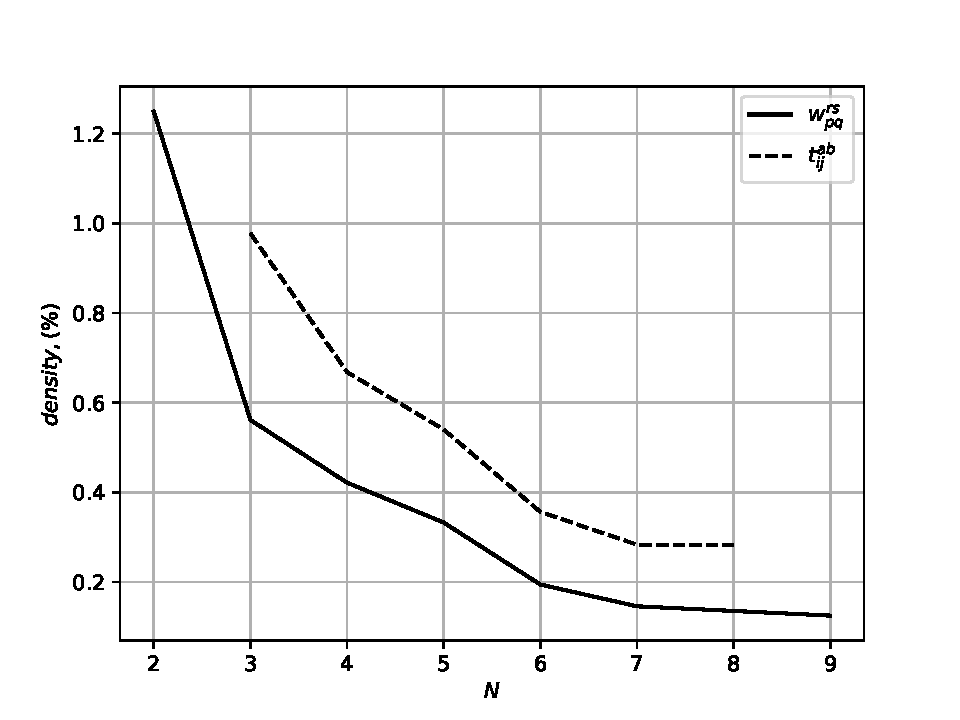
\includegraphics[width=0.7\linewidth]{density}
\caption{Density of the $T_2$ amplitudes and the two-body matrix elements for the 3D electron gas, given in percentages. $N$ denotes maximum value of the shell number. The amplitude density was estimated for 14 electrons.}
\label{fig:density}
\end{figure}

The same pattern is observed for the CCD amplitudes. On figure (\ref{fig:density}) it is easy to see that the density of non-zero amplitudes is quite low (below $1\%$). The most logical course for improving the brute force storing scheme(four-dimensional array) is to use some kind og mapping function(for example (\ref{simplemapping})) to create one-to-one correspondence between indices:
\begin{equation}
\bra{pq}\ket{rs} \rightarrow \braket{P||R}.
\end{equation} 
Now we can store matrix in computer memory instead of four-dimensional array. However we have not gained any significant performance yet, as we still store a lot of zeros. But taking into account density of the obtained matrix, we can treat it as so-called $sparce\ matrix$. There are several strict definitions of sparse matrix \cite{PissanetzkySparseMatrixTechnology2014}. However since our goal was not to write a sparse solver for CCD we just scratch the surface of this topic. We find sparse solver to be worth mentioning as it provides overview of the whole CC code optimization strategy:
\[
\begin{matrix} 
\text{brute-force solver:}\\
\text{CPU is not optimized}\\
\text{RAM is not optimized}\\
 \end{matrix} \rightarrow
 \begin{matrix} 
 \text{sparce solver:}\\
 \text{CPU is not optimized}\\
 \text{RAM is optimized}\\
\end{matrix} \rightarrow
 \begin{matrix} 
 \text{block solver:}\\
 \text{CPU is optimized}\\
 \text{RAM is optimized}\\
 \end{matrix}
\]
Sparse matrix can be written in a special form. As a simple example we can use coordinate list (COO) format. Name of format is self-explanatory: we store values and coordinates of the element, namely row and column indices in the following way:
\[
\begin{pmatrix} 

 0 & 1 & 1 & 0 & 0 & 0 \\
 1 & 0 & 0 & 0 & 0 & 0 \\
 0 & 0 & 0 & 0 & 0 & 0\\
 0 & 0 & 0 & 0 & 0 & 0\\
 0 & 0 & 0 & 0 & 7 & 0\\
 0 & 3 & 6 & 0 & 0 & 0 \\
\end{pmatrix} \rightarrow
\begin{pmatrix} 
1 & 1 & 3 & 1 & 6 & 7 \\
1 & 0 & 5 & 0 & 5 & 4 \\
0 & 1 & 1 & 2 & 2 & 3 \\
\end{pmatrix}
\begin{matrix} 
\leftarrow \mathrm{value} \\
\leftarrow \mathrm{row}\\
\leftarrow \mathrm{colomn}\\
\end{matrix}
\]

Summarizing we can use mentioned sparse matrix storage format for the reduction of the memory usage. The drawback of this method compared to the naive implementation might be in growing time for accessing needed elements.

Let us discuss a possible way to optimize the CPU time. We consider equation (\ref{CCDEnergy}) for the CCD correlation energy. Each pair of indices can be mapped into one:
\[
\begin{matrix} 
ij \rightarrow I \\
ab \rightarrow A \\
\end{matrix} 
\]

From now on, we denote the upper index, corresponding to the bra-part of the two-body matrix element, as a row index in the matrix representation. The lower index(ket-part) represents a column index. Tensor element $w_{ab}^{ij}$ has become matrix element $W_{A}^{I}$, that can be written in a more common way as $W_{AI}$.
Thus equation (\ref{CCDEnergy}) looks like:

\begin{equation}
\Delta E_{CCD} = \frac{1}{4} \sum_{IA} W_{A}^{I} T_{I}^{A} = \frac{1}{4} \sum_{IA} W_{AI} T_{IA} = \frac{1}{4} \text{trace}(W\times T),
\end{equation}

which is nothing else but the matrix-matrix multiplication. Thus the nested for-loops for evaluation of the sums can be replaced by fast linear algebra operations. Libraries like BLAS(Basic Linear Algebra Subprograms) are the obvious choice. However BLAS can multiply quickly only dense matrices, so we need either to create a fast library, which can multiply sparse matrices, or to use just a summation, instead of matrix-matrix multiplications.
Additionally we must note that not all diagrams in equation (\ref{ccdls}) can be easily replaced by the matrix products. For example we consider the fourth term:
\[
\hat{P}(ij|ab)\sum_{kc}w_{cj}^{kb}t_{ik}^{ac}.
\]

Before the matrix multiplication elements should be rearranged so that their indices match definition of the matrix-matrix multiplication. The resulting matrix must be rearranged back. We can conclude that this scheme is suited for the memory optimization but not the CPU optimization. In the next section we present so-called $block$ CCD solver which is both CPU and memory efficient. 

\section{The Block Implementation}
The block solver is much more abstract in comparison to the naive CCD solver. However it is the best one in a sense of optimization of both RAM- and CPU-usage. This is achieved through the utilization of the physical symmetries in the interaction.

The idea underlying this method is to take into account symmetries in the two-body interaction, for example, the angular momentum conservation or the spin conservation. Indeed, if we consider two-body matrix element $\braket{pq|\hat{v}|rs}$ it's easy to see, that it is non-zero only if two-body states $\ket{pq}$ and $\ket{rs}$ share the same quantum numbers. $\hat{v}$ acting to the right do not change quantum numbers of $\ket{rs}$, and the result is left-projected onto $\bra{pq}$. The similar property can be noted for the amplitudes, as they represent excitations due to the interaction, and, hence, $t_{ij}^{ab} \neq 0$ if a set of the quantum numbers for state $ij$ is the same as for $ab$. The last can be easily seen upon the initialization of the amplitudes. Equation (\ref{firsttarationamp}) provides the first guess for the amplitudes:
\begin{equation}\label{ampnonzero}
t_{ij}^{ab(0)} = \frac{w_{ab}^{ij}}{\epsilon_{ij}^{ab}}.
\end{equation}

Let us consider $ \frac{1}{2}\sum_{ab}w_{cd}^{ab}t_{ij}^{cd}$ term from equation (\ref{ccdls}). According to the discussion above it is possible to evaluate it as a matrix-matrix multiplication. Taking into account the symmetries of the interaction, the only non-zero terms in the result matrix are obtained from the matrix elements which correspond to the single-particle states obeying the following requirements:

\begin{equation}\label{constr1}
	\boldsymbol{k}_a + \boldsymbol{k}_b = \boldsymbol{k}_c + \boldsymbol{k}_d = \boldsymbol{k}_i + \boldsymbol{k}_j,
\end{equation}
and
\begin{equation}\label{constr2}
s_a + s_b = s_c + s_d = s_i + s_j.
\end{equation}

The obvious conclusion here is to construct the interaction matrix in a such way that its elements satisfy equations (\ref{constr1}) and (\ref{constr2}). In this case we avoid storing zero-elements and save the CPU time because there are no elements multiplied by zeros. The mentioned subsets of the TBME elements correspond to regions or $blocks$ in the matrix representation of the tensor describing the interactions.
The detailed analysis of the CCD amplitude equations shows that there are only terms where summations go over particle- or hole states. By definition the amplitudes are of the form particle-particle hole-hole. The two-body matrix elements are the elements of the form $\braket{pp||hh}$ $\braket{pp||pp}$ $\braket{ph||ph}$ etc. So it's naturally to split whole interaction matrix into blocks. This allows to save memory and utilize symmetries to avoid multiplication by zeros for all diagrams.
Additionally it is worse mentioning that all elements with repeated indices are zeros, for example $t_{ii}^{ab}$ or $\braket{pp|\hat{v}|rs}$.


\section{The Symmetry Channels}\label{sectionSymmetryChan}
As it has been shown in the previous section, construction of blocks obeying some particular symmetry laws is greatly improves numerical efficiency. In our system of interest(electron gas), these conservation laws are the conservation of the momentum and the conservation of the spin. For other systems these laws might be different. To generalize this discussion we define symmetry $channel$. Let us denote $(s_a + s_b)$ and $(\boldsymbol{k}_a + \boldsymbol{k}_b)$ from equations (\ref{constr1}) and (\ref{constr2}) as $S$ and $\boldsymbol{K}$ correspondingly. Pair of two-body state quantum numbers $(S, \boldsymbol{K})$ forms then so-called symmetry channel.

The general iterative procedure for solving the CCD, which is presented in listing (\ref{CCIteration}) is not changed. We need just to add a function which sets up channels before $while$-loop on line 2 and change methods for the calculation of the amplitudes and the correlation energy. To keep our CCD code more general, the amplitudes are set up in a different class. This is an obvious decision since channels reflect properties of the system. 

The single-particle state quantum numbers for electron gas are shown in table \ref{tab:spnumbers}. The simplest possible way to set up symmetry channels is to loop through all the combinations of the two-particle states and to check whether the quantum numbers are saved or not. We present this implementation in listing(\ref{CCSetUpChannels}). In our C++ code method \classname{setUpChannels}  from \classname{electrongaschannelset} class implements channel setup.

The result of this function is a vector of channels, where each channel contains two-body states obeying the symmetries of interactions.
In our implementation one symmetry channel is represented by an object of class \classname{channel}. Every instance of this class has a set of attributes which are vectors of index pairs of the states obeying symmetries in interaction.  
There are vectors of two-body states(represented by objects of class \classname{channelindexpair}) like ${particle\ minus\ hole}$. Additionally we need ${particle\ plus\ particle\ minus\ hole}$ and some other vectors. This is explained in more detail in the next section. 
\IncMargin{1em}
\begin{algorithm}[h!]
	\SetAlgoLined
	
	\SetKwData{Left}{left}\SetKwData{This}{this}\SetKwData{Up}{up}
	\SetKwFunction{Union}{Union}\SetKwFunction{FindCompress}{FindCompress}
	\SetKwInOut{Input}{input}\SetKwInOut{Output}{output}
	\Input{Single particle basis}
	\Output{Vector of matrices $\braket{pp||hh}$, $\braket{pp||hh}$ and $\braket{pp||hh}$}
	\BlankLine
	\emph{$N_{\mathrm{max}}$ - maximum shell number;}\;
	\emph{$S_{\mathrm{max}}$ = 2; SP spin value is $\pm 1$}\;
	\For{$N_x\leftarrow -N_{\mathrm{max}}$ \KwTo $N_{\mathrm{max}}$}{
		\For{$N_y\leftarrow -N_{\mathrm{max}}$ \KwTo $N_{\mathrm{max}}$}{  %{\label{forins}
			\For{$N_z\leftarrow -N_{\mathrm{max}}$ \KwTo $N_{\mathrm{max}}$}{
				\For{$S\leftarrow -S_{\mathrm{max}}$ \KwTo $S_{\mathrm{max}}$}{
					Create channel\\

						\For{$i\leftarrow 1$ \KwTo $N_{\mathrm{Fermi}}$}{
							\For{$j\leftarrow 1$ \KwTo $N_{\mathrm{Fermi}}$}{
								
								\If{$N_x,N_y,N_z,S$ $\mathrm{of\ state}$ $(i+j)$ = $N_x,N_y,N_z,S$}
								{add i,j to HoleHole vector}
						}
					}
					add HoleHole vector to Channel\\
						\For{$i\leftarrow 1$ \KwTo $N_{\mathrm{Fermi}}$}{
							\For{$a\leftarrow N_{\mathrm{Fermi}}$ \KwTo $N_{\mathrm{States}}$}{
								
								\If{$N_x,N_y,N_z,S$ $\mathrm{of\ state}$ $(i+a)$ = $N_x,N_y,N_z,S$}
								{add i,a to ParticleHole vector}
							}
						}					
					add ParticleHole vector to Channel\\
					$\dots$\\
					add ParticleParticle vector to Channel\\
					add HoleParticle vector to Channel\\
					add ParticleMinusHole vector to Channel\\
					add HoleMinusParticle vector to Channel\\


				}
			}
		}
	}
	\caption{Setting up symmetry channels for 3D electron gas.}\label{CCSetUpChannels}
\end{algorithm}\DecMargin{1em}

We should note that \classname{setupchannels} method is pure virtual, and\\ \classname{electrongaschannelset} is derived class. This allows to expand our code easily on other systems. To add a new system one needs to create a new derived class from the generalized class \classname{channelset} and implement \classname{setupchannels} method utilizing symmetries of this new system.

As it was already mentioned diagrams have no sum over all the states (particles and holes), thus the interaction matrix can be divided into blocks. All matrices are stored separately but are united by the channel. The interaction matrix can be split up into blocks as follows:

\[
\begin{pmatrix} 

         &\ket{hh} & \ket{ph} & \ket{hp} & \ket{pp}   \\
\ket{hh} & \braket{hh||hh} & \braket{hh||ph} & \braket{hh||hp} & \braket{hh||pp} \\
\ket{ph} & \braket{ph||hh} & \braket{ph||ph} & \braket{ph||hp} & \braket{ph||pp} \\
\ket{hp} & \braket{hp||hh} & \braket{hp||ph} & \braket{hp||hp} & \braket{hp||pp} \\
\ket{pp} & \braket{pp||hh} & \braket{pp||ph} & \braket{pp||hp} & \braket{pp||pp} \\

\end{pmatrix},
\]

where the first column and the first row denotes kind of vector holding particular type of states. For example $\ket{pp}$ is a vector that is made up from particle-particle states.

Summarizing, we store many small matrices or blocks for every symmetry channel instead of a four-dimensional array or a COO-formated matrix. 
In the \classname{ccd} class method \classname{setUpInterractionMatrixBlocks} provides a creation of the interaction matrix blocks. For every channel it takes the vectors of index pairs as an input, created as described in listing \ref{CCSetUpChannels}, and returns the interaction matrix blocks with unique link to each channel. In order to create a block corresponding to $\braket{hp||pp}$-type of interaction, we need to create a matrix for every channel by constructing it from the corresponding vectors. Row index of this matrix is given by the bra-part $\bra{hp}$, and column index is taken from the ket-part $\ket{pp}$. The value of the matrix element is calculated by \classname{TBME} method of the generalized \classname{SPBasis} class.

The CCD correlation energy is calculated as sum of traces of all matrices obtained by the multiplication of the corresponding interaction matrices and the amplitudes matrices within all channels. 
\IncMargin{1em}
\begin{algorithm}[h!]
	\SetAlgoLined
	
	\SetKwData{Left}{left}\SetKwData{This}{this}\SetKwData{Up}{up}
	\SetKwFunction{Union}{Union}\SetKwFunction{FindCompress}{FindCompress}
	\SetKwInOut{Input}{input}\SetKwInOut{Output}{output}
	\Input{Interaction matrix blocks and amplitude blocks}
	\Output{correlation energy}
	\BlankLine
	double CorrelationEnergy = 0.0 \\
	\For{$channelIndex \leftarrow 0$ \KwTo $ChannelVariety.size()$}{
		CorrelationEnergy += trace(m\_hhppVBlock.at(channelIndex).getMatrix()*\\m\_pphhTBlock.at(channelIndex).getMatrix())
	}
		return 0.25*CorrelationEnergy
	\caption{CCD correlation energy calculation for the channel solver.}\label{CCCorrChannels}
	\end{algorithm}\DecMargin{1em}


\section{Diagrams calculation}\label{sectiondiagcalc}

Up until then, we considered the simplest diagram $L_1$ and the CCD correlation energy expression in the context of the CPU optimization. The mentioned expressions have the ordering of the indices such as it is naturally and easy to notice matrix-matrix multiplication.
Let us consider $L_3$ term from equation (\ref{ccdls}):

\begin{equation}\label{eqL3}
	L_3 = \sum\limits_{kc}w_{cj}^{kb}t_{ik}^{ac}.
\end{equation}
Now it is not trivial to write this sum as matrix product. So reordering of the indices must be made:

\begin{equation}\label{decoupling}
 \sum\limits_{kc}w_{cj}^{kb}t_{ik}^{ac} \rightarrow \sum\limits_{kc}\tilde{w}_{jb}^{kc}\tilde{t}_{kc}^{ai}.
\end{equation}

Now it is obvious how to calculate sum in equation(\ref{decoupling}):
\begin{equation}
\tilde{L}_3 = \sum\limits_{kc}\tilde{w}_{jb}^{kc}\tilde{t}_{kc}^{ai} = \tilde{W}\times\tilde{T}.
\end{equation}
However this reordering cannot be implemented easily. One needs to take into account symmetries in the interaction. In the original $L_3$ term (\ref{eqL3}) the spin and the total momentum conservation must be satisfied for the following two-states sets of quantum numbers:
\begin{equation}\label{restrict}
	c + j = k + b = a + c = i + k.
\end{equation}
The elements of matrices $\tilde{W}$ and $\tilde{T}$ must satisfy the same restriction (\ref{restrict}). To do it we need to fill these matrices with the elements obeying the following conservation restriction: 

\begin{equation}\label{restrict1}
j - b = k - c = a - i = k - c,
\end{equation}
which is nothing else but relation (\ref{restrict}), written out according to the reordering scheme introduced in (\ref{decoupling}).
From the discussion above it follows that to calculate $L_3$ diagram as matrix product we need to construct interaction matrix block following restriction (\ref{restrict1}). This means that this matrix must be constructed from the vector containing the following two-body states: hole sp-state minus particle sp-state. This explains now the existence of lines (27-28) in listing (\ref{CCSetUpChannels}). We refer to the described procedure as $decoupling$. Some texts(links to Shean and Hansen) introduce term $alignment$ for this.
Finally we should mention that $\tilde{L}_3$ must be recoupled again to match the indexing scheme of amplitudes.

I the considered example pairs of states represent rows and columns. However $Q_3$ and $Q_4$ diagrams is impossible to decouple according to the similar scheme. To perform the calculation of these diagrams as matrix product, decoupling must be applied according the following scheme: the columns represent three states, and the rows represent one state. In table \ref{tab:recoupling} all decouplings are represented for the CCD block solver.

\begin{table}[h!]
	\caption{ Decoupling/Recoupling schemes for CCD diagrams.}
	\label{tab:recoupling}
	\begin{center}
		\begin{tabular}{cccccc}
			
			\hline
			\hline
			Name & Expression & Factor & Permutation & Decoupling & Re-coupling  \\
			\hline\\
			$  L_1 	  $  & $\sum\limits_{cd}w_{cd}^{ab}t_{ij}^{cd} $ & $  \frac{1}{2}$ &$  - $  & $w_{cd}^{ab}t_{ij}^{cd}  $ & $  -$  \\
			$  L_2    $  & $\sum\limits_{kl}w_{ij}^{kl}t_{kl}^{ab} $ & $  \frac{1}{2}$ &$  -  $  & $t_{kl}^{ab}w_{ij}^{kl}  $ & $  -$  \\
			$  L_3    $  & $\sum\limits_{kc}w_{cj}^{kb}t_{ik}^{ac} $ & $ 1 $ &$ \hat{P}(ij|ab)   $  & $ w_{ck}^{jb}t_{ai}^{ck} $ & $ L_{3\ ai}^{\prime\ jb} \rightarrow t_{ij}^{ab}$  \\
			$  Q_1    $  & $\sum\limits_{klcd}w_{cd}^{kl}t_{ij}^{cd}t_{kl}^{ab}  $ & $  \frac{1}{4}$ &$  -  $  & $t_{ij}^{cd}w_{cd}^{kl}t_{kl}^{ab} $ & $  -$  \\
			$  Q_2    $  & $\sum\limits_{klcd}w_{cd}^{kl}t_{ik}^{ac}t_{jl}^{bd} $ & $  1$ &$  \hat{P}(ij)  $  & $t_{ai}^{ck}w_{ck}^{ld}t_{ld}^{dj} $ & $  Q_{2\ ai}^{\prime\ dj} \rightarrow t_{ij}^{ab}$  \\
			$  Q_3    $  & $\sum\limits_{klcd}w_{cd}^{kl}t_{ik}^{dc}t_{lj}^{ab} $ & $  - \frac{1}{2}$ &$  \hat{P}(ij)  $  & $   t_{l}^{abj} w_{kcd}^{l}   t_{i}^{kcd}$ & $  Q_{3\ i}^{\prime\ abj} \rightarrow t_{ij}^{ab}$  \\
			$  Q_4    $  & $\sum\limits_{klcd}w_{cd}^{kl}t_{lk}^{ac}t_{ij}^{db} $ & $ - \frac{1}{2}$ &$ \hat{P}(ab)   $  & $t_{klc}^{a}   w_{d}^{klc}   t_{bij}^{d} $ & $ Q_{4\ a}^{\prime \ bij} \rightarrow t_{ij}^{ab}$  \\
		\end{tabular}
	\end{center}
\end{table}


\section{The block solver workflow}\label{blocksolvwf}
The pointer to the generalized basis class is passed to the solver, so that the methods inside the solver have access to the functions from the basis class. These functions are, for example, the calculation of the one- and two-body matrix elements, etc.
The benefit of this approach is the following: the solver has access to the special method, saying \classname{basis->TBME(p,q,r,s)}. If one wants to perform the CCD calculation of any other system(water molecule, quantum dot etc.), the only requirement is to create a new \classname{basis} derived class. Developer in this case is forced to create a new virtual function with prototype \classname{double TBME(int,int,int,int)} in this new derived class. And no modifications are required for the solver code. The same arguments can be mentioned for the class describing symmetry channels of the system.


\begin{figure*}[h!]
\begin{center}
	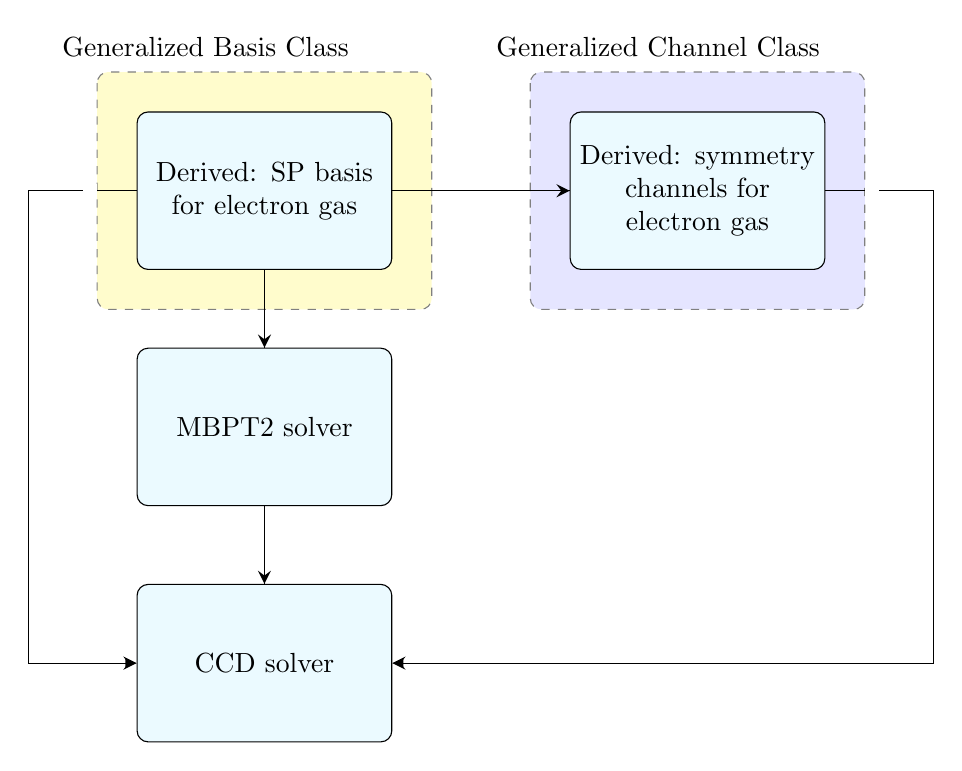
\begin{tikzpicture}[node distance=2cm]
	\node(CreateBasis)[roundrectSmall]{Derived: SP basis for electron gas};
	
	\node(CreateChannels)[roundrectSmall, right of=CreateBasis, xshift=3.5cm]{Derived: symmetry channels for electron gas};
	
	
	\node(MBPT2)[roundrectSmall, below of=CreateBasis, yshift=-1cm]{MBPT2 solver};
	
	\node(CCD)[roundrectSmall, below of=MBPT2, yshift=-1cm]{CCD solver};
	
	
	\draw [arrow] (CreateBasis) -- (CreateChannels);
	\draw [arrow] (CreateBasis) -- (MBPT2);
	\draw [arrow] (MBPT2) -- (CCD);
	
	\draw [arrow,rectangle connector=-3cm] (CreateBasis) to node[descr] [anchor=west]{} (CCD);
	\draw [arrow,rectangle connector=3cm] (CreateChannels) to node[descr] [anchor=east]{} (CCD);
	
	
	\begin{pgfonlayer}{background}
	% Compute a few helper coordinates
	\path (CreateBasis.west |- CreateBasis.north)+(-0.5,0.5) node (a) {};
	\path (CreateBasis.south -| CreateBasis.east)+(+0.5,-0.5) node (b) {};
	\path[fill=yellow!20,rounded corners, draw=black!50, dashed]
	(a) rectangle (b);
	\path (a.west |- a.north)+(+1.5,0.2) node (atext) {Generalized Basis Class};
	\end{pgfonlayer}
	
	
	\begin{pgfonlayer}{background}
	% Compute a few helper coordinates
	\path (CreateChannels.west |- CreateChannels.north)+(-0.5,0.5) node (a) {};
	\path (CreateChannels.south -| CreateChannels.east)+(+0.5,-0.5) node (b) {};
	\path[fill=blue!10,rounded corners, draw=black!50, dashed]
	(a) rectangle (b);
	
	\path (a.east |- a.north)+(+1.5,0.2) node (atext) {Generalized Channel Class};
	
	\end{pgfonlayer}
	%\caption{some fig}
	\end{tikzpicture}
\end{center}
		\caption{Classes needed for the CCD solver. } \label{fig:classes}
\end{figure*}



In our implementation, MBPT2 solver is used with symmetry channels. These channels are created inside the MBPT2 solver class. We need only particular state combinations, and the total number of channels is lower than one for the CCD solver. Thus standalone MBPT2 solver runs faster. However for the sake of generality, program architecture should be changed: MBPT2 solver should take channel setup as input.
The CCD solver needs knowledge about system, particularly, the single particle basis and the symmetry channels. Since CCD solver is iterative, it needs initial guess for the amplitudes and the correlation energy. The last two are provided by the MBPT2 solver. On figure \ref{fig:classes} the program work-flow is presented.

\section{Program structure and hierarchy}

We outline the structure of the program used for the calculations of the CCD equations for the electron gas in this thesis. We briefly describe functionality of the classes. For the detailed implementation of various methods we refer to the source code. All the names of functions, methods classes and variables were intended  to be self-explanatory. We hope that comments in the code can provide suitable illumination. Following classes are needed to perform calculations:

\begin{itemize}
	\item \classname{generalSPclass}

	\begin{itemize}
	\item \classname{electronGasSPBasis}

	
	\end{itemize}
	\item \classname{CartesianState}	
	\item \classname{channelset}
	\begin{itemize}
	\item \classname{electrongaschannelset}
	\end{itemize}
	\item \classname{channel}
	\item \classname{channelindexpair}
	\item \classname{symblock}
	\item \classname{ccd}
	\item \classname{mbpt2}
	\item \classname{mbpt2channels}
	
\end{itemize}
	
	
\subsection{Single-particle basis class}
	This is the base class containing pure virtual functions. Object of \classname{generalSPclass} is given as input for all solver classes to provide them with information about quantum system of interest. The two-body matrix elements of the Hamiltonian, single-particle energies, number of states and Fermi level are the typical quantities needed for almost every solver. %So this class contains prototypes for all the methods, that calculate....	
\subsection{The electron gas single-particle basis class}
	This class is derived class where the implementation of methods, described in \classname{generalSPclass},
	must be placed. As it follows from the name of this class it provides typical quantities of interest for the electron gas. The number of shells and electrons together with Wigner-Seitz radius are needed for the constructor, which calls two methods: \classname{setUpUnits} and \classname{setUpStatesCartesian}. That creates a vector of objects \classname{CartesianState}, where each object represents a single-particle state as a set of quantum numbers(see table \ref{tab:spnumbers}).
	 \classname{setUpUnits} function is needed to create output of such key quantities as, for example, energy in atomic units. The other important methods which are heavily used in other classes are:
\begin{itemize}
\item \classname{TBME} returns anty-symmetrized two-body matrix elements of the Hamiltonian. For the electron gas it is simply hard-coding of equation (\ref{TBMEHEG}).
\item \classname{getQuantumStates}, \classname{getQuantumStatesNumber} and \\ \classname{calculateReferenceEnergy} functions provide an useful information fo debug purposes.
\item \classname{computeSPenergies} returns vector with the single-particle energies in the Hartree-Fock basis.
\item \classname{sumState}, \classname{substractState} are used for channels setup in CCD solver and for the symmetry restriction check in CCQMC solver. These functions make a sum or a difference of two single-particle states. 
\end{itemize}


\subsection{Single-particle state class}
Every instance of \classname{CartesianState} class is a set of four integers, representing $n_x$, $n_y$, $n_z$ and $s$. Generally, this is a small class which acts like a data structure in C++. Our motivation to have it as a separate class is based on a possibility to consider Cartesian state as a derived class of some generalized class. That improves generalization of the code by allowing to include easy other coordinate systems or dimensionalities.

\subsection{Symmetry channels class}
Base class for setting up the symmetry channels, which contains virtual functions only.
For the CCD solver there are three functions. 
\begin{itemize}
\item \classname{setUpChannels}
\item \classname{setUpChannelsQ3}
\item \classname{setUpChannelsQ4}
\end{itemize}
\classname{setUpChannels} sets up channels for $L_1$ -- $Q2$ diagrams. Notation we use for different diagrams can be found in table \ref{tab:recoupling}.

\subsection{The electron gas symmetry channels class}
Implementation of the setup of the symmetry channels for the electron gas is located in this class. We have actually already covered this topic in section \ref{sectionSymmetryChan}.



\subsection{Channel class}\label{channelsection}
Instances of this class act as an organized storage for single-particle states\footnote{strictly speaking, we store indices of single-particle states in \classname{m_shells} vector.}. 
Objects of this class contain a set of vectors. Each vector corresponds to the particular interaction, which must obey symmetry constrains. These vectors are:
\begin{itemize}
\item \classname{m_HoleHoleVec}
\item \classname{m_ParticleParticleVec}
\item \classname{m_ParticleHoleVec}
\item \classname{m_ParticleMinusHoleVec}
\item \classname{m_HoleParticleVec}
\item \classname{m_HoleMinusParticleVec}
\item \classname{m_ParticlePlusParticleMinusHoleVec}
\item \classname{m_HoleVec}
\item \classname{m_HolePlusHoleMinusParticleVec}
\item \classname{m_ParticleVec}
\end{itemize}
Each element in mentioned vectors is an object of class \classname{channelindexpair}. For example, we consider amplitude $t_{ij}^{ab}$. As we know the value of this amplitude is non-zero if the following constrain is satisfied:
\begin{equation}
i + j = a + b,
\end{equation} 										
for both the momentum and the spin. We store all hole-state indices $i$ and $j$ as a pair for a given channel in \classname{m_HoleHoleVec}. Similarly we do with particle-state indices $a$ and $b$ and vector \classname{m_ParticleParticleVec}. We must apology here for a not a completely strict name of class  \classname{channelindexpair}, as it can hold one or even three indices, which are needed for the diagrams $Q_3$ and $Q_4$.

\subsection{Symmetry block class}\label{symblocksection}
This class is used for the interaction matrices. The main purpose is to structure interactions for each channel into a matrix. It also serves the purpose of the creation of the index vectors, where we store one-to-one correspondence between the interaction matrix element and single-particle state number.
Vectors with symmetry block objects are created inside \classname{ccd} solver class.
Since coupled cluster amplitudes are stored on the same form, this class is used to create amplitudes matrices with mapping as well.

\subsection{CCD solver class}\label{ccdsolversec}

the main method of the \classname{ccd} class is \classname{iterateCCD}. Here one can find the main component of the CCD solver, which is iterative procedure, shown in listing \ref{CCIteration}.
To start iterations we initialize interaction matrix blocks and amplitude matrices. It is done by the following functions:
\begin{itemize}    
\item    \classname{setUpInterractionMatrixBlocks}
\item    \classname{setUpInitialAmplitudes}
\item    \classname{setUpInterractionMatrixBlocksQ3}
\item    \classname{setUpInitialAmplitudesQ3}
\item    \classname{setUpInterractionMatrixBlocksQ4}
\item    \classname{setUpInitialAmplitudesQ4}
\end{itemize}

Result of these functions is a set of vectors with \classname{symblock} objects. The complete list of these vectors is presented below:


\begin{table}[h!]

	\begin{center}
		\begin{tabular}{ll}
			\classname{m_hhhhVBlock}	& \classname{m_pphhTBlock} \\ 
			\classname{m_ppppVBlock}	& \classname{m_pphhTBlockPrev} \\ 
			\classname{m_hMphMpVBlock}	& \classname{m_pMhhMpTBlock} \\ 
			\classname{m_hhppVBlock}	&  \classname{m_pMhhMpTBlockPrev}\\ 
			\classname{m_hMppMhVBlock}	& \classname{m_ppMhTBlock} \\ 
			\classname{m_ppMhVBlock}	& \classname{m_ppMhTBlockPrev} \\ 
			\classname{m_hhMpVBlock}	&  \classname{m_hhMpTBlock}\\ 
			\classname{m_pphhVBlock}	& \classname{m_hhMpTBlockPrev}\\
	\end{tabular} 
	\end{center}
\end{table}

They are filled up in a such way that every \classname{symblock} object in any of mentioned vector has the index which matches index of the channel. The most important data is stored in the interaction matrix of the \classname{symblock} object. For certain channels some matrices, of course, are impossible to construct. 

Inside the CCD iteration amplitudes are calculated and updated by the following functions: \classname{calculateAmplitudes} and \classname{updateAmplitudes}. Inside these functions amplitudes are calculated by the evaluation of the diagrams term by term, sometimes including decoupling and recoupling, that was described in section \ref{sectiondiagcalc}.

     
\subsection{MBPT2 classes}
\classname{mbpt2} class is a brute-force implementation of the MBPT2 equations via sums and for-loops. This class can be useful as a unit test when adding new systems to the code.
\classname{mbpt2channels} class serves as input for the CCD solver. It is a small class with two major methods: \classname{setUpChannels} and \classname{calculateEnergyMatMult}. Reasons for having a separate function to setup symmetry channels in side this class were presented in section \ref{blocksolvwf}.

\section{Possible optimization}

\subsubsection{Intermediates}

So-called $intermediates$ provides us with a way of achieving reduction of execution time of our CCD code.
According to \cite{MillerQuantumMechanicalStudies2017} speed up gained by using them can reach values up to 25\% which is a significant improvement. What is even more important is the usage of the intermediates for higher truncation levels.
The basic idea is to find common quantities for different diagrams calculated repeatedly during one iteration. It seems to be logical to calculate these quantities only once in the beginning of each iteration and reuse them later for a diagram. As an example, we consider the last diagram of equation (\ref{ccdls}):
\begin{equation}
	Q_4 = -\frac{1}{2}\hat{P}(ab)\sum_{klcd}w_{cd}^{kl}t_{lk}^{ac}t_{ij}^{db} = -\frac{1}{2}\hat{P}(ab) \sum_{c} t_{ij}^{ac} \sum_{kld} w_{cd}^{kl} t_{kl}^{bd} = -\frac{1}{2}\hat{P}(ab) \sum_{c} t_{ij}^{ac} I,
\end{equation}
where intermediate $I$ defined by equation (\ref{I4}) and it is calculated only once during iteration.
\begin{equation}\label{I4}
	I = \sum_{kld} w_{cd}^{kl} t_{kl}^{bd}
\end{equation}
Considered $Q_4$ computed without intermediates must be calculated for all $t_{ij}^{ab}$, and it is easy to see that this operation scales as $\mathcal{O} (N_{particles}^4\cdot N_{holes}^4)$ number of flops. Implementation of intermediate \ref{I4} reduces power of $N_{holes}^4$ by two.

\subsubsection{Mapping}

To calculate permutations and to update amplitudes we need to know where elements should be placed in the original matrix. In the end of CCD iteration we obtain amplitudes in a form of $t_{ij}^{ab}$ (particle + particle = hole + hole), so we need to know which elements to place into, for example, (particle - hole = hole - particle) matrix, which is needed for $L_3$ diagram. In addition to that information about place in the new matrix is needed. \classname{getRowMap} and \classname{getRowMap} functions have the simplest posible implementation for these mentioned one-to-one correspondence. Given \classname{channelindexpair} object as an input, they return an integer index, so we know where this object is located in the mapping matrix. Code listing on figure \ref{fig:L3update} shows how these functions are called.
We planned to use hash tables from the standard library and store \classname{ChannelIndexPair} as value and index as a key. That could provide us with a faster search algorithm. However due to an unexpected bug, we have not managed to make it work.
\begin{figure}
\begin{lstlisting}[language=C++]
for(unsigned int chan = 0; chan < ChannelVariety.size(); chan++){
 	channel onechannel = ChannelVariety.at(chan);
   	symblock amplitudes = m_pMhhMpTBlock.at(chan);
   	for(unsigned int ai = 0; ai < onechannel.m_ParticleMinusHoleVec.size(); ai++){
   		for(unsigned int jb = 0; jb < onechannel.m_HoleMinusParticleVec.size(); jb++){
   			int a = amplitudes.getRowMap(ai).first();
   			int i = amplitudes.getRowMap(ai).second();
   			int j = amplitudes.getColMap(jb).first();
   			int b = amplitudes.getColMap(jb).second();
   			double value = updateAmplitudesL3(a,b,i,j);
   			m_pMhhMpTBlockPrev.at(chan).setElement((int)ai, (int)jb, value);
   		}
   	}
}
\end{lstlisting}
\caption{Update of $L_3$ diagram.}\label{fig:L3update}
\end{figure}

Mapping of channels with unique value of $\mathbf{k}$ should be considered as an alternative scheme for the organization of channels.
As it was already described in sections \ref{ccdsolversec}, \ref{channelsection} and \ref{symblocksection}, we create a vector of channel objects, where each one contains information about unique value of interaction symmetry. When calculating one chosen diagram, say $L_3$, loop goes over all channels in \classname{ChannelVariety} vector and calculates $L_3$ with the code presented on figure \ref{fig:L3}. It can be seen from the listing that a simple storing scheme for channels by bonding them to the ascending index of the vector element comes with a drawback that is absence of flexibility. Each particular channel does not necessarily contains all possible block-matrices. In the listing there is check if they contains non-zero \classname{m_ParticleMinusHoleVec} and \classname{m_HoleMinusParticleVec} blocks. Instead it can be much more efficient to go through channels that already have these non-zero blocks.

\begin{figure}
\begin{lstlisting}[language=C++]
void ccd::L3(){
	for(unsigned int chan=0; chan < ChannelVariety.size(); chan++)
	{
		channel onechannel = ChannelVariety.at(chan);
		if (onechannel.m_ParticleMinusHoleVec.size()*
			onechannel.m_HoleMinusParticleVec.size() != 0)
			{
			m_pMhhMpTBlock.at(chan).setMatrix(
			m_pMhhMpTBlockPrev.at(chan).getMatrix()*
			m_hMphMpVBlock.at(chan).getMatrix());
			}
	}
}
\end{lstlisting}
\caption{$L_3$ diagram calculation.}\label{fig:L3}
\end{figure}

Each channel can be distinguished from other by its unique combination of quantum numbers(lets denote them as $U_i$). We can iterate before the channel setup and check how many $U_i$ combinations exist. After that it can be created an one-dimensional array of symmetry block objects with a link between $U_i$ and index of an object in this array. Afterward some mapping can be created, where we connect indices in the array with particular non-zero blocks.

\subsubsection{Parallelization}

Message Passing Interface(MPI) and Multi Processing(MP) are tools which come to mind last, after all mathematical optimization is implemented. MPI is a standard developed for the distributed memory architectures, while MP is is an application programming interface used for the shared memory architecture.



All mentioned optimization technicalities were skipped in our implementation as the main goal of the CCD solver was to produce the benchmark information for CCQMC solver. We are able to run simple calculations for the 3D electron gas with 14 electrons up to 13 shells on a typical personal computer.



\section{Occupation Number Representation of SD}\label{occnumrep}
We consider a common energy diagram and show how it is possible to translate it into occupation number representation. 
\begin{figure}[!ht]\label{plot1f}
		\begin{center}
			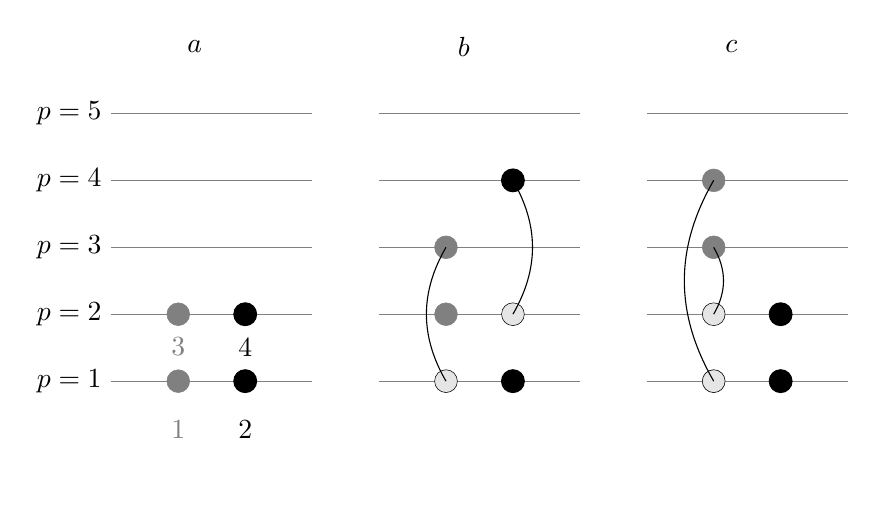
\begin{tikzpicture}[scale=0.85]
			\begin{scope}[xshift=4cm]
			\draw (0.5,5) node[anchor=east] {$a$};
			\foreach \i in {1,...,5}
			{
				\draw (-1,\i-1) node[anchor=east] {$p = \i$} --(2,\i-1);
			}
			\foreach \i in {1,...,5}
			{
				\draw[gray,very thin] (-1,\i-1) --(2,\i-1);
			}
			
			\filldraw[gray,very thin] (0,0) node[anchor=north,inner sep=.5cm] {$1$} circle (0.17cm);
			\filldraw (1,0) node[anchor=north,inner sep=.5cm] {$2$} circle (0.17cm);
			\filldraw[gray,very thin] (0,1) node[anchor=north,inner sep=.3cm] {$3$} circle (0.17cm);
			\filldraw (1,1) node[anchor=north,inner sep=.3cm] {$4$} circle (0.17cm);
			\end{scope}

			\begin{scope}[xshift=8cm]
			\draw (0.5,5) node[anchor=east] {$b$};
			\foreach \i in {1,...,5}
			{
				\draw[gray,very thin] (-1,\i-1) --(2,\i-1);
			}
			\draw[fill=gray!20!white, very thin] (0,0)  circle (0.17cm);
			\filldraw (1,0)  circle (0.17cm);
			\filldraw[gray,very thin] (0,1) circle (0.17cm);
			\draw[ fill=gray!20!white, very thin] (1,1) circle (0.17cm);
			\filldraw[gray,very thin] (0,2) circle (0.17cm);
			\filldraw (1,3) circle (0.17cm);
			\draw (0,0) to[gray,very thin,bend left] (0,2);
			\draw (1,1) to[gray,very thin,bend right] (1,3);			
			\end{scope}
		\begin{scope}[xshift=12cm]
		\draw (0.5,5) node[anchor=east] {$c$};
		\foreach \i in {1,...,5}
		{
			\draw[gray,very thin] (-1,\i-1) --(2,\i-1);
		}
		\draw[gray,very thin] (0,0)  circle (0.17cm);
		\filldraw (1,0)  circle (0.17cm);
		\draw[ fill=gray!20!white, very thin] (0,0) circle (0.17cm);
		\filldraw[gray,very thin] (0,2) circle (0.17cm);
		\filldraw (1,1) circle (0.17cm);
		\draw[fill=gray!20!white, very thin] (0,1) circle (0.17cm);
		\filldraw[gray,very thin] (0,3) circle (0.17cm);
		\draw (0,0) to[gray,very thin,bend left] (0,3);
		\draw (0,1) to[gray,very thin,bend right] (0,2);
		\end{scope}			
			
			\end{tikzpicture}
		\end{center}
		\caption{The open-shell electron gas with four electrons and five energy levels. All states with spin up are gray, the opposite spin states are black. The labeling scheme of the single-particle states is shown on figure (a). }\label{figureOCCNUM}
	\end{figure}

Let us consider a simple example of a system with four electrons and five energy levels. The reference determinant is shown on figure \ref{figureOCCNUM}(a). It is possible to represent reference as a sorted array where index of each element refers to the state number, and its value reflects the information if this state is filled with the particle or not.
For example, the determinant corresponding to figure \ref{figureOCCNUM}(a) can be written as follows:
\[
\ket{D_0} = \ket{\phi_1 \phi_2 \phi_3 \phi_4} = \ket{1_1 1_2 1_3 1_4 0_5 0_6 0_7 0_8 0_9 0_{10} }.
\]
Storing the array of integers, which can have just two values(0 and 1), is not an optimal way since 32 or 64 bits are required to store one integer number in memory. The best solution is to use bit-strings here, which are just a sequence of bits. Every bit can have just two values: 0 or 1.
Since there is no smaller unit of information than bit, it is the most memory-efficient way to store Slater determinants. It can be crucial for us as the full space of the determinants is formed as $\binom {2M}{N}$, where $N$ is number of the occupied orbitals out of $2M$ orbitals.

In C++ we used \classname{BOOST} \classname{dynamic_bitset} library as it allows to create bit-strings of dynamic size in contradiction to the standard library where the length of the bit-string must be defined during compilation time.
The side effect of the occupation number representation of determinants as a bit-strings is inbuilt implementation of the second-quantized excitation operators through bitwise operation XOR(of course, up to sign). For example, we look at \ref{figureOCCNUM}(b) where particle 1 is exited to state number 5 and particle from 4 is exited to state 8. To generate the determinant corresponding to \ref{figureOCCNUM}(b) we act with two excitation operators $\hat{a}_1^5 \hat{a}_4^8$ on the reference. In the bit-string representation, excitations the operators look as follows:
\[
1_1 0_2 0_3 1_4 1_5 0_6 0_7 1_8 0_9 0_{10}.
\]
Applying this string through XOR operation to the reference we obtain exited determinant up to sign:
\[
\begin{matrix} 
	&1001100100 \\
	XOR& \\
	&1111000000\\
	&\downarrow \\
	&0110100100\\
\end{matrix}
\]
Additionally we need to stress that the occupation numbers represent only one of the $N!$ determinants, which are possible to make from $\phi_1$ to $\phi_N$ single-particle functions. To illustrate this we show simple example for $N=3$:
\[
\ket{11001} = \ket{1,2,5} = -\ket{2,1,5} = -\ket{5,2,1} = -\ket{1,5,2} = \ket{2,5,1} = \ket{5,1,2}.
\]
All these determinants are clearly linearly dependent.

To be consistent with the mathematical formalism describing action of creation/annihilation operators we need to determine sign. By definition the action of these operators on the determinant is written as follows:
\[
\hat{a}_i \ket{a,b,\dots, i,\dots} = (-1)^{i-1} \ket{a,b,\dots, \bcancel{i},\dots},
\]
and
\[
\hat{a}^\dagger_i \ket{a,b,\dots, j, \dots} = (-1)^{i-1} \ket{a,b,\dots, i,j,\dots}.
\]
Later in this chapter it is shown that we operate with the following excitation operators:
\[
\hat{t}_{ij...k}^{ab...c} = \hat{a}^\dagger_a \hat{a}^\dagger_b ... \hat{a}^\dagger_c \hat{a}_k ... \hat{a}_j \hat{a}_i,
\]
where $i<j<...<k$ and $a<b<...<c$.
Hence the application of this excitor to the reference might result in a change of sign, i.e:
\[
\hat{t}_{ij}^{ab} \ket{D_0} = -\ket{D_{ij}^{ab}}.
\]

As a more concrete example, let us consider a set of states with the reference $\ket{D_0} = \ket{1,2,3}$. The action of two different exitors, $ \hat{t}_{13}^{58}$ and $\hat{t}_{12}^{58}$, is written out explicitly:

\begin{align*}
   \hat{t}_{13}^{58} \ket{1,2,3} &= + \hat{a}^\dagger_5 \hat{a}^\dagger_8 \hat{a}_3 \hat{a}_1 \hat{a}^\dagger_1 \hat{a}^\dagger_2 \hat{a}^\dagger_3 \ket{-}\\
                         &= + \hat{a}^\dagger_5 \hat{a}^\dagger_8 \hat{a}_3 \hat{a}^\dagger_2 \hat{a}^\dagger_3 \ket{-}\\
                         &= - \hat{a}^\dagger_5 \hat{a}^\dagger_8 \hat{a}_3 \hat{a}^\dagger_3 \hat{a}^\dagger_2 \ket{-}\\
                         &= - \hat{a}^\dagger_5 \hat{a}^\dagger_8 \hat{a}^\dagger_2 \ket{-}\\
                         &= + \hat{a}^\dagger_5 \hat{a}^\dagger_2 \hat{a}^\dagger_8 \ket{-}\\
                         &= - \hat{a}^\dagger_2 \hat{a}^\dagger_5 \hat{a}^\dagger_8 \ket{-}\\
                         &= - \ket{2,5,8}\\
\end{align*}
\begin{align*}
           \hat{t}_{12}^{58} \ket{1,2,3} &= + \hat{a}^\dagger_5 \hat{a}^\dagger_8 \hat{a}_2 \hat{a}_1 \hat{a}^\dagger_1 \hat{a}^\dagger_2 \hat{a}^\dagger_3 \ket{-}\\
                                 &= + \hat{a}^\dagger_5 \hat{a}^\dagger_8 \hat{a}_2 \hat{a}^\dagger_2 \hat{a}^\dagger_3 \ket{-}\\
                                 &= + \hat{a}^\dagger_5 \hat{a}^\dagger_8 \hat{a}^\dagger_3 \ket{-}\\
                                 &= - \hat{a}^\dagger_5 \hat{a}^\dagger_3 \hat{a}^\dagger_8 \ket{-}\\
                                 &= + \hat{a}^\dagger_3 \hat{a}^\dagger_5 \hat{a}^\dagger_8 \ket{-}\\
                                 &= + \ket{2,5,8}
\end{align*}






\section{CCQMC Cluster Size}

In \autoref{CCQMCChap} we showed that instead of the direct integration of the  imaginary-time Schr\"{o}dinger equation we rewrite it in a such way, that it is possible to sample it. Using the coupled cluster expansion we can determine amplitudes as iteration procedure from time $\tau$ to ($\tau + \delta \tau$): 
\begin{equation}\label{CCbf3new}
t_{\{i\}}(\tau + \delta \tau) = t_{\{i\}}(\tau) - \delta \tau \langle D_{\{i\}}|(\hat{H}-E)|\Psi_{CC}(\tau)\rangle.
\end{equation}
To simulate this equation one needs to sample the coupled cluster wavefunction:

\begin{equation}\label{WFtosmple}
\Psi_{CC}(\tau) = \big[1 + \sum_{\textbf{\mathrm{i}}} \underbrace{t_{\textbf{\mathrm{i}}}\hat{a}_{\textbf{\mathrm{i}}}}_{\text{size 1}} + \sum_{\textbf{\mathrm{ij}}} \underbrace{t_{\textbf{\mathrm{i}}} t_{\textbf{\mathrm{j}}} \hat{a}_{\textbf{\mathrm{i}}} \hat{a}_{\textbf{\mathrm{j}}}}_{\text{size 2}} + \sum_{\textbf{\mathrm{ijk}}}\underbrace{t_{\textbf{\mathrm{i}}} t_{\textbf{\mathrm{j}}} t_{\textbf{\mathrm{k}}} \hat{a}_{\textbf{\mathrm{i}}} \hat{b}_{\textbf{\mathrm{j}}} \hat{a}_{\textbf{\mathrm{k}}}}_{\text{size 3}} + \dots  \big] \ket{D_0}
\end{equation}

We choose a single term from expansion (\ref{WFtosmple}) at the time. This process is known as the collapse of the wavefunction to the cluster. We define cluster size by the number of excitors it contains: $t_{\textbf{\mathrm{i}}}\hat{a}_{\textbf{\mathrm{i}}}$ corresponds to the cluster of size one, $t_{\textbf{\mathrm{i}}} t_{\textbf{\mathrm{j}}} \hat{a}_{\textbf{\mathrm{i}}} \hat{a}_{\textbf{\mathrm{j}}}$ represents the cluster of size two, etc. 
 
We set maximal cluster size to be three. Additionally we consider just single, double and, possibly, triple excitations. That means that the cluster of size three is just three single excitations, while cluster of size one can be single, double or triple excitation. The detailed relations between the cluster size and the excitation level are shown in table \ref{tab:cpluster}.  


\begin{table}[h!]
	\caption{ Cluster size and excitation level. Table explains how we can construct cluster of certain size using different excitation operators. For example, cluster of size three can be constructed just from single excitation to avoid reaching higher excitations than level three. }
	\label{tab:cpluster}
	\begin{center}
		\begin{tabular}{ccccc}
			
			%\hline
			\hline
			cluster size & Single & Double & Triple  \\
			\hline\\
			$ 0 $ & $-$ & $-$ & $-$ &   \\
			$ 1 $ & $S$ & $D$ & $T$ &   \\
			$ 2 $ & $SS$ & $DS/SD $ & $-$ &   \\
			$ 3 $ & $SSS$ & $-$ & $-$ &   \\
		\end{tabular}
	\end{center}
\end{table}

\section{CCQMC Solver}

As it was already mentioned in \autoref{CCQMCChap}, we use a variable $N_0$(see equation(\ref{eq:exptauloop})) to preserve the intermediate normalization.
If we omit $\tau$ - dependence(we consider the exponential ansatz of the wave-function during one $\tau$ - iteration), the expansion of the coupled cluster wavefunction (\ref{WFtosmple}) becomes the following:
\begin{equation}\label{CCQMCcode}
\ket{\Psi_{CC}} = \big[N_0 + \sum_{\textbf{\mathrm{i}}} t_{\textbf{\mathrm{i}}}\hat{a}_{\textbf{\mathrm{i}}} + \frac{1}{N_0 2!}\sum_{\textbf{\mathrm{ij}}} t_{\textbf{\mathrm{i}}} t_{\textbf{\mathrm{j}}} \hat{a}_{\textbf{\mathrm{i}}} \hat{a}_{\textbf{\mathrm{j}}} + \frac{1}{N_0^2 3!}\sum_{\textbf{\mathrm{ijk}}}t_{\textbf{\mathrm{i}}} t_{\textbf{\mathrm{j}}} t_{\textbf{\mathrm{k}}} \hat{a}_{\textbf{\mathrm{i}}} \hat{b}_{\textbf{\mathrm{j}}} \hat{a}_{\textbf{\mathrm{k}}} + \dots  \big] \ket{D_0}.
\end{equation}
We can refer to $N_0$ as the population of excips on the reference. However it is not true, because these excips are not the same kind of excip, populating the excitation space.
In equation (\ref{eq:exptauloop}) the cluster operator $\hat{T}$ is by definition:
\begin{equation}
\hat{T}(\tau) = \hat{T}_1(\tau) + \hat{T}_2(\tau) + \hat{T}_3(\tau) + \dots,
\end{equation}
where, for example, $\hat{T}_2(\tau)$ contains all the double-orbital replacements of the reference determinant through excitors $\hat{a}_{\textbf{\mathrm{i}}}$:
\begin{equation}
\hat{T}_2 = \sum_{\textbf{\mathrm{j}}\ \in\ \text{double replacements} } t_{\textbf{\mathrm{j}}}(\tau) \hat{a}_{\textbf{\mathrm{j}}}, 
\end{equation}
where $t(\tau)$ is a parametrization of the exponential expansion of the wavefunction. In the deterministic coupled cluster theory we used equations (\ref{linkedCCampl}) to find their values. In the CCQMC we use similar to the DMC method by considering a population of walkers $N_w$. Each walker is located on determinant $\textbf{j}_\alpha$ and have sign $s_{\alpha} = \pm $. We define amplitude $t_{\textbf{i}}$ to be proportional to the population of walkers. It is important that population sign of walkers is taken into account:
\begin{equation}
t_{\textbf{\mathrm{i}}} \propto N_i = \sum_\alpha s_\alpha \delta_{i,i_\alpha}.
\end{equation}
However total population is simply a sum of absolute values of the populations of all walkers:
\begin{equation}
N_w = \sum_i |N_i|.
\end{equation}

We outline the general structure of the CCQMC solver. 
We simulate equation (\ref{CCbf3new}). This is performed by the \classname{applyCCQMC} method of the \classname{ccqmc} class.
As it has been already mentioned, to evaluate a non-trivial term  $\langle D_{\{i\}}|(\hat{H}-E)|\Psi_{CC}(\tau)\rangle$ from equation (\ref{CCbf3new}) we perform two sampling processes. They are the sampling of the wavefunction (\ref{CCQMCcode}) and the sampling of the action ot the Hamiltonian. The possible strategy here is to choose randomly clusters from the wavefunction (\ref{WFtosmple}) such, that the cluster size follows the exponential distribution:
\begin{equation}\label{expdistrib}
	p_{size}(s)=\frac{1}{2^{s+1}},
\end{equation}
where $s$ is a cluster size.
Instead we sample each cluster size separately. So during one $\delta\tau$ iteration we call consistently functions \classname{sampleReference}, \\ \classname{sampleClusterSizeOne} and \classname{sampleClusterSizeTwo}. The sampling of the action of the Hamiltonian is included in these functions and will be covered below. The result of these mentioned function is a two vectors: \classname{TemporaryStorage} consisting of exitors and \classname{TemporaryStoragePopulation} which holds the population of excipts on these exitors. During annihilation step in the end of the $\tau$-loop, these vectors are being merged with \classname{StorageCumulativeDeterminants} and \classname{StorageCumulativePopulation}. Exitors with no excips are deleted from \classname{StorageCumulativeDeterminants} vector. The last is crucial since the length of the \classname{StorageCumulativeDeterminants} vector is used in sampling. Described above procedure is presented in listing \ref{CCQMCloop} in terms of pseudo-code.


\IncMargin{1em}
\begin{algorithm}%[H]
	\SetAlgoLined
	
	\SetKwData{Left}{left}\SetKwData{This}{this}\SetKwData{Up}{up}
	\SetKwFunction{Union}{Union}\SetKwFunction{FindCompress}{FindCompress}
	\SetKwInOut{Input}{input}\SetKwInOut{Output}{output}
	\Input{$\delta\tau$-timestep, max value of $\tau_{max}$, initial population $N_0$}
	\Output{Vector with population, vector with exitors}
	\BlankLine
	%\emph{special treatment of the first line}\;
	
	\For{$\tau \leftarrow 0$ \KwTo $\tau_{max}$}{

		sampleReference $N_0$ times \\
		sampleClusterSizeOne $\frac{2}{3}N_{ex}$ times \\
		sampleClusterSizeTwo $\frac{1}{3}N_{ex}$ times \\
		merge current population with total population \\
		annihilation step \\
		$\tau = \tau + \delta\tau$\\
		
	}
	\caption{The CCQMC iteration.}\label{CCQMCloop}
\end{algorithm}\DecMargin{1em}











\section{CCQMC Sampling}



Because of the complicity of the sampling procedure, it might be best to present simplified block diagram. We present it on figure \ref{figccqmcWF}. Bearing in mind this diagram, one can delve into technicalities of the sampling scheme for the CCQMC algorithm.
The sampling of the wavefunction involves two random events.
First, we select cluster size $s$ randomly, according to the exponential distribution (\ref{expdistrib}). In our implementation we sample different cluster sizes various number of times.
Second, $s$ excitors are selected within the chosen cluster size. In this case the conditional probability to choose $s$ excitors is stands as:
\begin{equation}\label{condprob}
p_{\text{clust}} (e|s)= s! \prod_{i=1}^s \frac{|N_i|}{N_{ex}},
\end{equation}
where factor $s!$ represents the number of permutations in the construction of a cluster.
%Factor $s$ introduces the number of permutations that might be used to obtain the same cluster from different excitors.
$N_{ex}$ is the total number of the exitors which can by sampled in the system(doubles, if we choose the CCD truncation). According to the multiplication theorem on probability, one can sample all possible combinations of excitors with the total probability:
\begin{equation}\label{eq:pselect}
p_{select}^{cluster}(e)= p_{size}(s) p_{\text{clust}} (e|s) =  \frac{s!\prod_{i=1}^{s} |N_i|}{2^{s+1}N_{ex}}.
\end{equation}
So one sample of the wavefunction can be described by equation (\ref{eq:pselect}), and we use this sample $N_a$ times. So, naturally, one definite cluster can be sampled with probability $\frac{1}{N_a}$. %__!!__without choosing a size and following choosing of cluster within this size.__!!__
However it is easy to notice that the mentioned above two random processes will change $N_a$ so, that it decreases. In this case the probability is $\frac{1}{N_a^\prime}$, where $N_a^\prime = N_a p_{select}^{cluster}$.
After the wavefunction collapsed to cluster, the result is $\Psi_{CC}(\tau)\ \rightarrow\ A\ket{D_m}$,
where $A$ is an amplitude of the constructed cluster and is defined as follows:
\begin{equation}
A = N_0  \prod_{i=1}^s \frac{N_i}{N_0},
\end{equation}
where $N_i$ is the population of excips on the excitor $i$. 
The last term of equation (\ref{CCbf3new}) is now simplified into the following expression:
\begin{equation}\label{simplesampling}
\delta \tau A \langle D_{\{i\}}|(\hat{H}-S)\ket{D_m}
\end{equation}
According to the described in \autoref{CCQMCChap} scheme, the sampling of the action of the Hamiltonian is performed by choosing random single or double excitation of $\ket{D_m}$ for the bra-part $D_{\{i\}}$. We denote obtained determinant as $D_n$. The Hamiltonian matrix element then became $\langle D_n|\hat{H}\ket{D_m} = H_{nm}$. The expression (\ref{simplesampling}) is simplified as follows:
\begin{equation}\label{physprob}
\delta \tau A H_{nm}
\end{equation}
We spawn an excip on $D_n$ determinant with a probability proportional to (\ref{physprob}), which includes the physics of the system. However we used quite complicated series of random events to obtain expression (\ref{physprob}). So to unbias sampling we need to include combinatorics probabilities for the spawning of an excip. We multiply $\delta \tau A H_{nm}$ by the probability discussed above:  $\frac{1}{N_a^\prime}$, and the probability for spawning is defined by the following expression:
\begin{equation}
\delta \tau A H_{nm} \frac{1}{N_a p_{select}^{cluster}} = \delta \tau A H_{nm} \frac{1}{N_a p_{size}(s) p_{\text{clust}} (e|s)}.
\end{equation}

The only remaining factor is the probability for choosing bra-part during the sampling of the action of the Hamiltonian. Thus the final probability for spawning can be written as follows:


\begin{equation}
P_{\text{spawn}} = \underbrace{\delta \tau |A H_{nm}|}_{\text{physics}} \underbrace{\frac{1}{N_a p_{size}(s) p_{\text{clust}} (e|s)}}_{\text{sampling ket-part}} \underbrace{\frac{1}{P_{gen}}}_{\text{sampling bra-part}},
\end{equation}
where $P_{gen}=\frac{1}{N_{s+d}}$ is the probability to choose single or double excitation among all available.

The probability for excip to be killed/cloned is proportional to the diagonal matrix elements of the Hamiltonian:
\begin{equation}
P_{\text{death}} = \delta \tau | A (H_{nn}-S) | \frac{1}{N_a p_{size}(s) p_{\text{clust}} (e|s)} ,
\end{equation}

\newpage

\begin{figure}[!h]
\begin{center}
	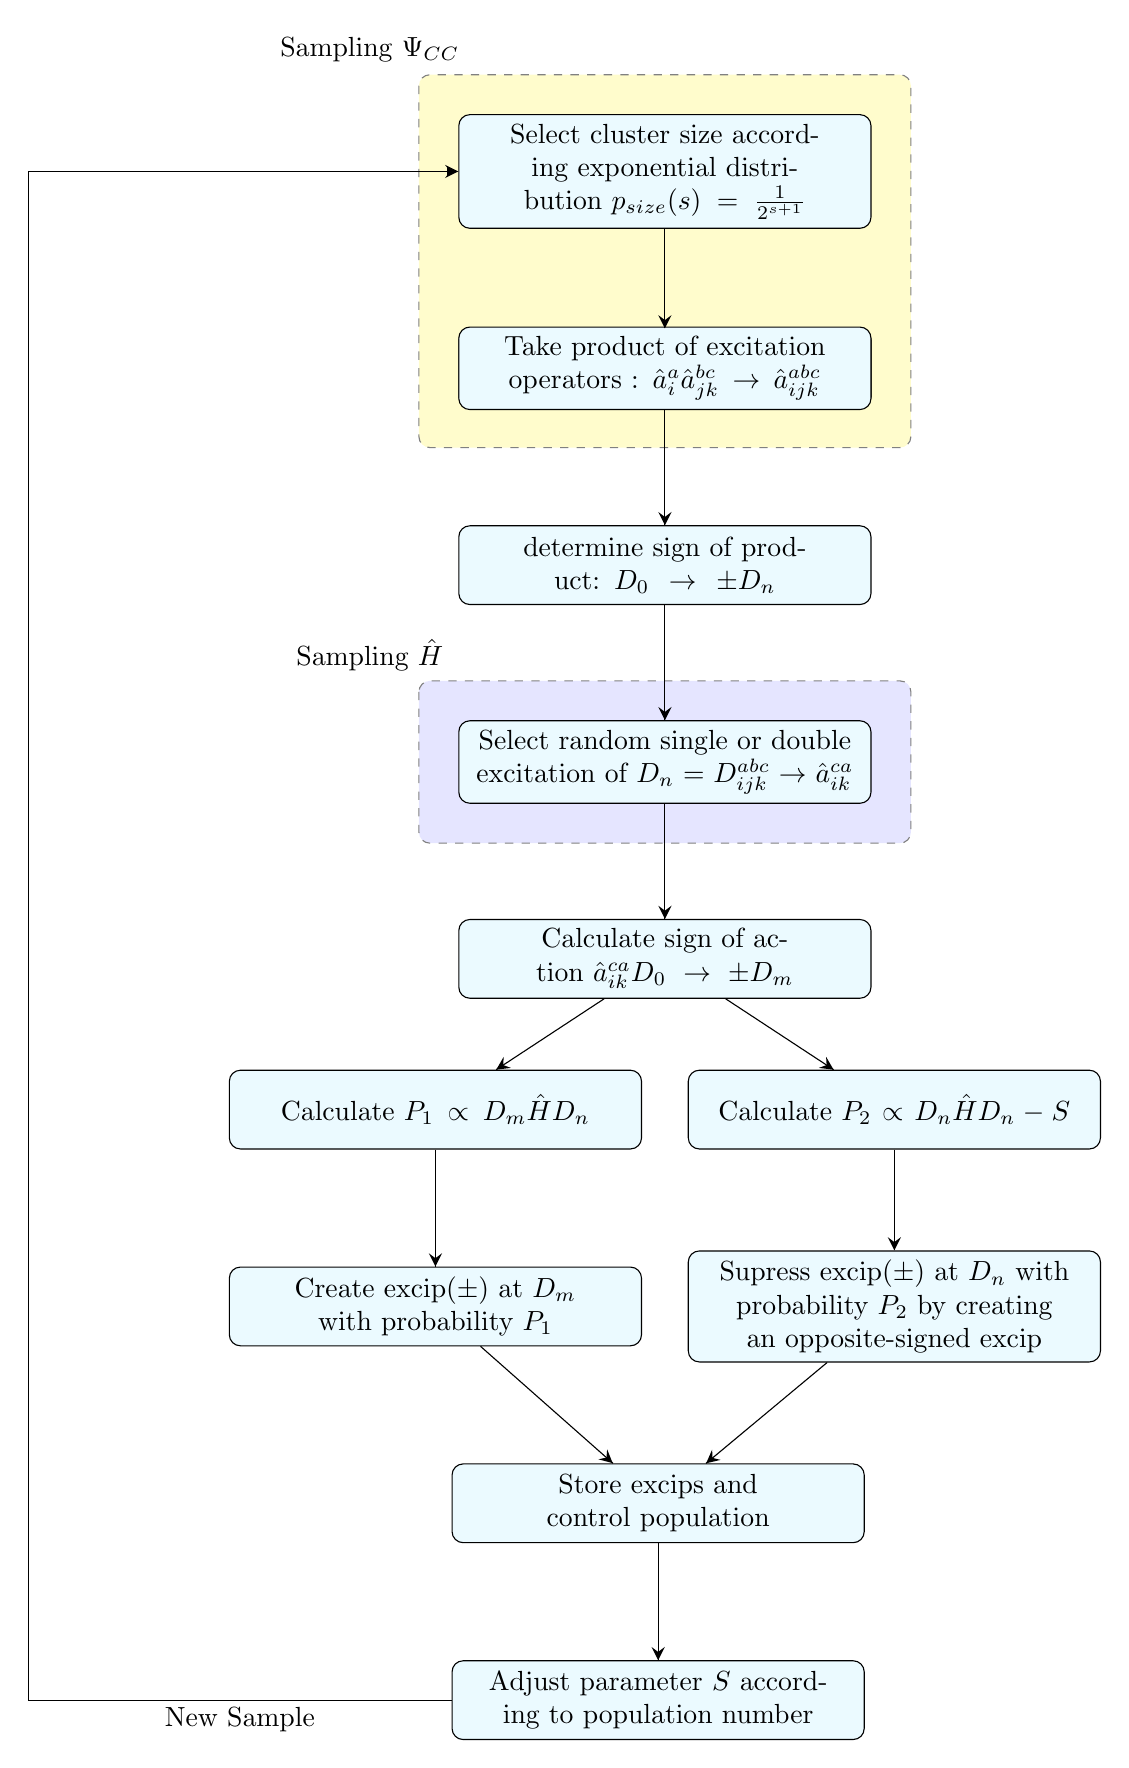
\begin{tikzpicture}[node distance=2cm]
	\node(SelectCluster)[roundrect]{Select cluster size according exponential distribution $p_{size}(s)=\frac{1}{2^{s+1}}$};% of one particle in one dimension};
	\node(ConstructCluster)[roundrect, below of=SelectCluster, yshift=-0.5cm]{Select excitations according to rules from tab. \ref{tab:cpluster}};
	\node(ProductCluster)[roundrect, below of=SelectCluster, yshift=-0.5cm]{Take product of excitation operators : $\hat{a}_{i}^{a}\hat{a}_{jk}^{bc} \rightarrow \hat{a}_{ijk}^{abc}$};
	\node(KetSign)[roundrect, below of=ProductCluster, yshift=-0.5cm]{determine sign of product: $\ket{D_0} \rightarrow \pm \ket{D_n}$};
	\node(SelectBra)[roundrect, below of=KetSign, yshift=-0.5cm]{Select random single or double excitation of $\ket{D_n} = \ket{D_{ijk}^{abc}} \rightarrow \hat{a}_{ik}^{ca}$};
	\node(BraSign)[roundrect, below of=SelectBra, yshift=-0.5cm]{Calculate sign of action $\hat{a}_{ik}^{ca}\ket{D_0} \rightarrow \pm \ket{D_m} $ };
	\node(Offdiagonal)[roundrect, below left of=BraSign, yshift=-0.5cm, xshift=-1.5cm ]{Calculate $P_1 \propto \bra{D_m}\hat{H} \ket{D_n}$};
	\node(Diagonal)[roundrect, below right of=BraSign, yshift=-0.5cm,xshift=1.5cm]{Calculate $P_2 \propto \bra{D_n}\hat{H} \ket{D_n}-S$};
	\node(CreateExcip)[roundrect, below of=Offdiagonal, yshift=-0.5cm]{Create excip($\pm$) at $\bra{D_m}$ with probability $P_1$};
	\node(KillExcip)[roundrect, below of=Diagonal, yshift=-0.5cm]{Supress excip($\pm$) at $\ket{D_n}$ with probability $P_2$ by creating an opposite-signed excip};
	\node(StoreExcip)[roundrect, below of=KillExcip, yshift=-0.5cm, xshift=-3cm]{Store excips and control population};
	\node(TuneS)[roundrect, below of=StoreExcip, yshift=-0.5cm]{Adjust parameter $S$ according to population number};
	\draw [arrow] (SelectCluster) -- (ConstructCluster);
	\draw [arrow] (ConstructCluster) -- (ProductCluster);
	\draw [arrow] (ProductCluster) -- (KetSign);
	\draw [arrow] (KetSign) -- (SelectBra);
	\draw [arrow] (SelectBra) -- (BraSign);	
	\draw [arrow] (BraSign) -- (Offdiagonal);
	\draw [arrow] (BraSign) -- (Diagonal);
	\draw [arrow] (Offdiagonal) -- (CreateExcip);
	\draw [arrow] (Diagonal) -- (KillExcip);
	\draw [arrow] (KillExcip) -- (StoreExcip);
	\draw [arrow] (CreateExcip) -- (StoreExcip);
	\draw [arrow] (StoreExcip) -- (TuneS);
	\draw [arrow,rectangle connector=-8cm] (TuneS) to node[descr] [anchor=north]{New Sample} (SelectCluster);
	%	\draw [arrow] (Check E) -- node [anchor=east]{Yes} (Finish);
	%\background{Setup system}{Set T2}{Calc CCDT}{Calc D10}{Wave-function}
	%\background{Setup system}{Set T2}{Calc CCDT}{Calc D10}{Wave-function}
	\begin{pgfonlayer}{background}
	% Compute a few helper coordinates
	\path (SelectCluster.west |- SelectCluster.north)+(-0.5,0.5) node (a) {};
	\path (ConstructCluster.south -| ConstructCluster.east)+(+0.5,-0.5) node (b) {};
	\path[fill=yellow!20,rounded corners, draw=black!50, dashed]
	(a) rectangle (b);
	\path (a.west |- a.north)+(-0.5,0.2) node (atext) {Sampling $\ket{\Psi_{CC}}$};
	\end{pgfonlayer}
	\begin{pgfonlayer}{background}
	% Compute a few helper coordinates
	\path (SelectBra.west |- SelectBra.north)+(-0.5,0.5) node (a) {};
	\path (SelectBra.south -| SelectBra.east)+(+0.5,-0.5) node (b) {};
	\path[fill=blue!10,rounded corners, draw=black!50, dashed]
	(a) rectangle (b);
	\path (a.west |- a.north)+(-0.5,0.2) node (atext) {Sampling $\hat{H}$};
	\end{pgfonlayer}
	\end{tikzpicture}
\end{center}
\caption{CCQMC sampling work-flow. } \label{figccqmcWF}
\end{figure}
\clearpage

\section{Sampling of the action of the Hamiltonian}
The sampling of the action of the Hamiltonian is performed by choosing random single or double excitation of collapsed wavefunction $\ket{D_m}$ for the bra-part $D_{\{i\}}$. We denote obtained determinant as $D_n$.

For double excitation one can write:
\begin{equation}
\ket{D_{m}}=a^\dagger_r a^\dagger_s a_q a_p \ket{D_n}, 
\end{equation}
where orbitals $p,q$ are chosen from the occupied set of orbitals, while $r,s$ are selected from the unoccupied orbitals with respect to the $D_n$. Conditional probability is then can be written as follows:
\begin{equation}\label{pdouble}
p_{gen}(n|m) = p(r,s|p,q)p(p,q),
\end{equation}
where $p(p,q)$ is the probability to select pair $p,q$ in $D_n$, and $p(r,s|p,q)$ is the probability to select pair $r,s$ in condition that pair $p,q$ is selected.
According to the Slater-Condon rules we can select a single excitation of $\ket{D_m}$ as well. In this case, denoting this excitation as:
\begin{equation*}
\ket{D_{m}}=a^\dagger_r  a_p \ket{D_n},
\end{equation*}
the expression for the probability can be written:
\begin{equation}
p_{gen}(n|m) = p(r|p)p(p).
\end{equation}
In general $p_{gen}(n|m)$ is calculated using either double or single excitation:
\[
p_{gen}(n|m)=\left\{
\begin{array}{ll}
p(r,s|p,q)p(p,q) \cdot P_{\text{double}}, \ \text{for double excitation}\\
p(r|p)p(p) \cdot (1-P_{\text{double}}), \ \text{for single excitation},
\end{array}
\right.
\]
where factors $P_{\text{double}}$ and $(1-P_{\text{double}})$ were used for normalization. $P_{\text{double}} \in (0,1)$ represents probability of choosing double excitation. For the electron gas it is not possible to choose single excitation, and, hence, $p_{gen}$ is defined by equation (\ref{pdouble}).

Let us consider the second factor of equation (\ref{pdouble}), representing the probability to select pair $p,q$ in $D_n$. For the $N$-particle the probability to select $uniformly$ a pair is the following:
\begin{equation}
p(p,q) = {\binom{N}{2}}^{-1} = \frac{2}{N(N-1)}.
\end{equation}
Now we consider conditional probability $p(r,s|p,q)$ from equation (\ref{pdouble}). Having selected $p$ and $q$, we could either choose $r$ and then $s$ or vice versa.

\begin{equation}\label{condprob1}
p(r,s|p,q) = p(r|s,p,q)p(s|p,q) + p(s|r,p,q)p(r|p,q).
\end{equation}
We select $s$ orbital with probability $p(s|p,q)$ given that we have already selected pair $p,q$. After this we choose the second orbital with the probability $p(r|s,p,q)$. A similar line of reasoning is applied to the second term in equation (\ref{condprob1}). $p(s|p,q)$ is defined by the number of available orbitals, that fulfill certain constrains. For considered system these are the conservation of momentum and spin. So for given $p,q$ pair we need to check if orbital $s$ satisfy:
\begin{equation}
|\boldsymbol{k}_p + \boldsymbol{k}_q - \boldsymbol{k}_s|  < R_F,
\end{equation} 
which reflects that a combination of quantum numbers lies within the Fermi sphere.
For the electron gas the fourth orbital is completely defined by the selection of the previous three, and hence, the remaining probability is:

\begin{equation}
p(r|s,p,q) = p(s|r,p,q) = 1.
\end{equation}

\section{The Hamiltonian matrix elements}

For double excitation:
\begin{equation}
\ket{D_{m}}=a^\dagger_r a^\dagger_s a_q a_p \ket{D_n}.
\end{equation}
In this case the corresponding matrix element then is:
\begin{equation}
\bra{D_n} \hat{H}\ket{D_{m}}=\braket{rs|pq}_{AS}.
\end{equation}
For single excitation:
\begin{equation}
\ket{D_{m}}=a^\dagger_r  a_p \ket{D_n}.
\end{equation}
And corresponding matrix element then is:
\begin{equation}
\bra{D_n} \hat{H}\ket{D_{m}}=\sum_{k}^{N-1}\braket{rk|pk}_{AS},
\end{equation}
where summation goes over all common orbitals  for $D_n$ and $D_m$.
The diagonal matrix elements are calculated with the following expression:
\begin{equation}
\bra{D_n} \hat{H}\ket{D_{n}}=\sum_{p\in n} \langle p|\hat{h}|p\rangle + \frac{1}{2} \sum_{p,q \in n}^{N-1}\braket{pq|pq}_{AS}.
\end{equation}

\section{The sign of excip}
 The signs of the excips and their progeny are crucial for the successful CCQMC simulations. In addition to the explicit minus sign in the propagation equation (\ref{common0}), one should consider the following sources of the sign change:
 
 \begin{enumerate}
 	
 	\item The sign of the Hamiltonian matrix element $H_{nm}$.
 	
 	\item The sign of the parent excip. In the case of the composed cluster the sign of the amplitude of this cluster must be considered. The amplitude of the excips on a cluster of excitors is the product of the individual amplitudes, corresponding to the excitors, which construct the cluster.
 	
 	\item Combining excitors to form a cluster, we perform reordering of the creation/annihilation operators. Odd number of such permutations causes a sign change in the excip population.
 	
 	\item Applying the randomly chosen excitor to the reference can result in a sign change. This was described in \autoref{occnumrep}.  
 	
 	\item Sampling the action of the Hamiltonian, we choose the excited determinant in the bra-part. This determinant is a result of the action of some excitor on the reference. Thus if we consider spawning an excip on the excitor which create this determinant, we must take into account the sign of the excitor relative to the reference determinant.
 \end{enumerate}
 
 In order to observe the correct dynamics, we must carefully accumulate all negative signs and take them into account before spawning an excip.


\section{CCQMC code structure}

 We were not able to find any description of the CCQMC algorithm implementation in literature. To our knowledge there is the only one implementation exists, developed by the authors of the algorithm. When we started writing code we knew not a lot about technicalities of CCQMC implementation. Therefore, we decided to start with just one class and keep code as simple as possible to illuminate potential sources of errors.
 
 When coded we were guided by the paradigm formulated by Kent Beck, "Make it work, make it right, make it fast". When implementing the couple cluster doubles truncation for the electron gas we found it difficult to split solver into classes. It was found later that the class separation is necessary for including other systems and higher truncation levels.
 
 The main difficulty if CCQMC algorithm is to implement the sign structure of wavefunction correctly. While we use bitstring representation of determinants, we found it useful to start with a vector representation. Below we present a code that can help to understand the basic concept, however it should be considered as a kind of unit test and not a part of the algorithm. We consider determinant $\ket{D}_{ij}^{ab}$ as a small vector, where we write all creation/annihilation operators in a predetermined order. We look at the following example:

\begin{equation*}
\ket{D}_{ij}^{ab} \rightarrow [ i,j\ \vdots \ a,b]
\end{equation*}
 This is helpful as it allows to construct the exact creation/annihilation string of operators in correct order:
 \begin{equation*}
[ i,j \ \vdots \ a,b] \rightarrow \hat{c}^\dagger_a \hat{c}^\dagger_b \hat{c}_i \hat{c}_j.
 \end{equation*}
If during sampling we choose excitor $\hat{c}^\dagger_a \hat{c}^\dagger_b \hat{c}_j \hat{c}_i$, which by action on the reference collapses the wavefunction into $-\ket{D}_{ji}^{ab}$. Vector representations of mentioned excitors will be different:
\begin{equation*}
[ i,j\ \vdots \ a,b] \neq [ j,i\ \vdots \ a,b].
\end{equation*}
This slows down algorithm significantly, however eliminates one source of errors: we don't need to obtain the phase by acting with one annihilation/creation operator on the given Slater determinant.
 
\begin{figure}[h!]
\begin{lstlisting}[language=C++]
auto it = find_if(TemporaryStorage.begin(), TemporaryStorage.end(), [&SampledCluster](const std::vector<int>& EachDet) {return std::search(EachDet.begin(), EachDet.end(), SampledCluster.begin(), SampledCluster.end()) != EachDet.end();});
if (it != TemporaryStorage.end()){
auto index = std::distance(TemporaryStorage.begin(), it);
TemporaryStoragePopulation.at((index)) += (-1)*SignOfCluster;
} else {
TemporaryStorage.push_back(SampledCluster);
TemporaryStoragePopulation.push_back((-1)*SignOfCluster);
}
\end{lstlisting}
\caption{Finding of Slater determinant in vector representation.}\label{fig:CCQMCfindDetVector}
\end{figure}


to be continued:\\

%ideas:\\
% 
% So solver takes a basis class as an input with the condition that odd/even indices of single particle states corresponds to states with different spins.
%
% While we began with writing general code for including at least single, double and triple excitations, we ended with functions for the double excitations only with lost of generality.








\section{Possible optimization}
Based on our observations the $better$ way to write the CCQMC solver is to split different parts of the algorithm into the class structure described below.
First of all calculation of $P_gen$ probabilities may differ for various systems, so the code for this task must be a part of the basis class.
The purpose of the main solver class should be implementation of the main imaginary-time loop, possibly, with a role of the MPI load balancer.
Vectors with populations and determinants is better to keep as a separate class, which makes it more flexible to change between storage data types and search algorithms. It can definitely be needed during debugging phase in the development of code and benchmarking of the results.

Advantages of the parallel computing is natural to use for Monte Carlo methods. Number of samples can be increased by the factor of number of CPU cores without considerable increase of the execution time. However parallelization of the algorithm should be implemented with care. The first problem might be increased covariance caused by the quality of random number generator. The second is a load balancing scheme, which we propose below.
Master process performs initial sampling and creates an object with populations and determinants. Then each MPI-child process receives a copy of this object. Sampling of all cluster sizes is performed independently by each child process and sent back to the master without any additional data processing.
After all the objects with populations and determinants are gathered, master process performs annihilation step by merging all objects into collective storage at this particular imaginary-time step. This require a significant amount of CPU time and can be speed up by OpenMP and a smart algorithm for sorting/searching elements in arrays. 
Also, it should be noted that during annihilation step child processes are in a "sleep" state. It happens because of the fact, they need an updated list with excips and their total number to start new sampling.

This study has found that development of the code for the CCQMC algorithm requires continuous monitoring of different parameters during simulations. This usually includes number of spawning/death events, sign of spawned excips, total number of positive/negative death occurrences, event distribution over cluster size etc.
We suggest that output of debug information should be separated into a standalone class, and developer must pay particular attention to it. In our simulations we used a simple approach of appending a datafile in the end of every $\tau$-loop. Python environment was then employed to produce real-time plots. Plotting directly from C++ may be the best choice here due to speed of disk write operations.  

\chapter{Results and Discussion}






\section{CCD benchmark}

The brute force solvers written in Python and C++ are slow. They were used to compare contribution of different diagrams or to test permutations under development of the block solver. However for larger basis sizes and growing number of particles it was not possible to compare results with brute-force solvers.

CCD approximation for the electron gas has been extensively studied by many researchers. An obvious way to validate our results is to compare CCD correlation energy with energies of other codes. We compared our energies to the results of Hansen\cite{HansenCoupledclusterstudies},  Baardsen \cite{BaardsenCoupledclustertheoryinfinite2014} and recent studies of Miller\cite{MillerQuantumMechanicalStudies2017}. Our code produced results which corroborate the findings of a great deal of the previous work, as can be seen in table \ref{tab:CCDcompar}.




However comparison of results with precision beyond 6 digits might be useful only for specific debug purposes. We used $10^{-6}$ tolerance for the iterative process. Besides, precision of different constants \footnote{We refer here to the Planck constant, the speed of light, the fine-structure constant etc. which are used in \classname{setUpUnits} function fo the electron gas.} used to set up units correctly is usually determined to about the 5-8th decimal. Additionally taking into account round-off errors or minor differences in the implementation, we think that agreement in results of other codes up to the $10^{-6}$ due to precision -- eto fakt, po kotoromy my schitaem rezultaty correktnymi.
It is apparent from this table that the results are consistent within mentioned numerical precision.

\begin{landscape}

\begin{table}[h]
	\centering
	\captionsetup{width=.8\textwidth}
	\caption{CCD results comparison between our block CCD solver ($\Delta E_{CCD}^M$), Millers's results, Hansen's CCD results ($\Delta E_{CCD}^H$) for the HEG. Results of Baardsen ($\Delta E_{CCD}^B$).	Results are presented for $14$ electrons. Mixing parameter $\alpha=0.8$ for Miller's results, and $\alpha=0.3$ for Hansen's and our results. All energies are presented in Hartree units.} \label{tab:CCDcompar}
	\begin{tabular}{rrllll}
		$r_s$ & States & $\Delta E_{CCD}$ \cite{MillerQuantumMechanicalStudies2017} & $\Delta E_{CCD}$ \cite{HansenCoupledclusterstudies} & $\Delta E_{CCD}$ \cite{BaardsenCoupledclustertheoryinfinite2014} & $\Delta E_{CCD}$\\
		\hline
		\hline
            1.0 & 54 & -0.3178228436889338 & -0.317822843688933   &           & -0.3178230699319593  \\
            1.0 & 66 & -0.3926965898061968 & -0.3926965898061966  &           & -0.3926968074770886  \\
            1.0 & 114 & -0.4479105961757175 & -0.4479105961757175 & -0.447909 & -0.4479109389185165  \\
            1.0 & 162 & -0.4805572589306421 & -0.4805572589306416 &           & -0.4805570782443642  \\
            1.0 & 186 & -0.4855229317521320 & -0.4855229317521318 & -0.485523 & -0.4855227418241649  \\
            1.0 & 246 & -0.4929245740023971 & -0.4929245740023975 &           & -0.4929243692209991  \\
            1.0 & 294 & -0.4984909094066806 & -0.4984909094066818 &           & -0.4984906939593084  \\
            1.0 & 342 & -0.5019526761547777 & -0.5019526761547779 &           & -0.5019524529049425  \\
            1.0 & 358 & -0.5025196736076414 & -0.502519673607641  & -0.502523 & -0.5025194488388953  \\ \hline
            0.5 & 114 & -0.5120153541478306 & -0.5120153541478306 & -0.512015 & -0.5120152296730573  \\
            0.5 & 186 & -0.5114620616957333 &                     & -0.553329 & -0.553329520936615   \\
            0.5 & 342 & -0.5729645498903680 & -0.572964549890367  &           & -0.572964399507112   \\
            0.5 & 358 & -0.5297417436322546 &                     & -0.573678 & -0.5736804143578936  \\ \hline    
            2.0 & 114 & -0.3577968843144996 & -0.3577968843144996 & -0.357798 & -0.3577955282575226  \\
            2.0 & 342 & -0.4014136184665558 & -0.4014136184665555 &           & -0.4014117905655014  \\
	\end{tabular}
\end{table}

\end{landscape}


As a simple unit test we compare our results for a small number of electrons with the result of the CCD solver from \cite{Hjorth-Jensenadvancedcoursecomputational2017}. The table \ref{tab:unittest} illustrates agreement in the correlation energy up to 15 significant digits of precision.

\begin{table}[h]
\centering
\captionsetup{width=.8\textwidth}
\caption{CCD iteration comparison with solver from \cite{Hjorth-Jensenadvancedcoursecomputational2017} for the HEG. Here, $N_e=2$, $N_s=66$, $r_s=1.0$, and there is no mixing. }
        	\begin{tabular}{rlll}
        		n & $\Delta E_{CCD}$     & $\Delta E_{CCD}$ \cite{Hjorth-Jensenadvancedcoursecomputational2017} \\
        		MBPT2 & -0.02080623248720259 & -0.0208062324872026  \\
        		0 & -0.01833394188507821 & -0.0183339418850782  \\
        		1 & -0.01864313296809337 & -0.01864313296809333 \\
        		2 & -0.01860449158525421 & -0.01860449158525414 \\
        		3 & -0.01860932269795203 & -0.01860932269795206 \\
        		4 & -0.01860871870720909 & -0.01860871870720907 \\
\end{tabular}
\label{tab:unittest}
\end{table}
                              



\section{Thermodynamic limit estimates}

In the thermodynamic limit (TDL) the density of the electron gas remains constant while the particle number tends to infinity($N\rightarrow \infty$). However many-body methods scales relatively expensive with $N$. Calculations for large $N$ were performed by several researchers and are available in a few codes with extensive parallelism. Dazhe nesmotra na eto only finite systems can be studied. Typical strategy is to to begin with $N$ electrons in a simulation-cell, and approach the thermodynamic limit using extrapolation techniques.

The second difficulty arises from the fact that the many-body wavefunction is constructed from a finite one-particle basis set. By introducing limited number of single-particle states($M$) we limit kinetic energy values for the electron gas. Strictly, both limits should be found: TDL($N\rightarrow \infty$) and complete basis set(CBS) limit($M \rightarrow \infty$)

\begin{figure}[ht!]
	\centering
	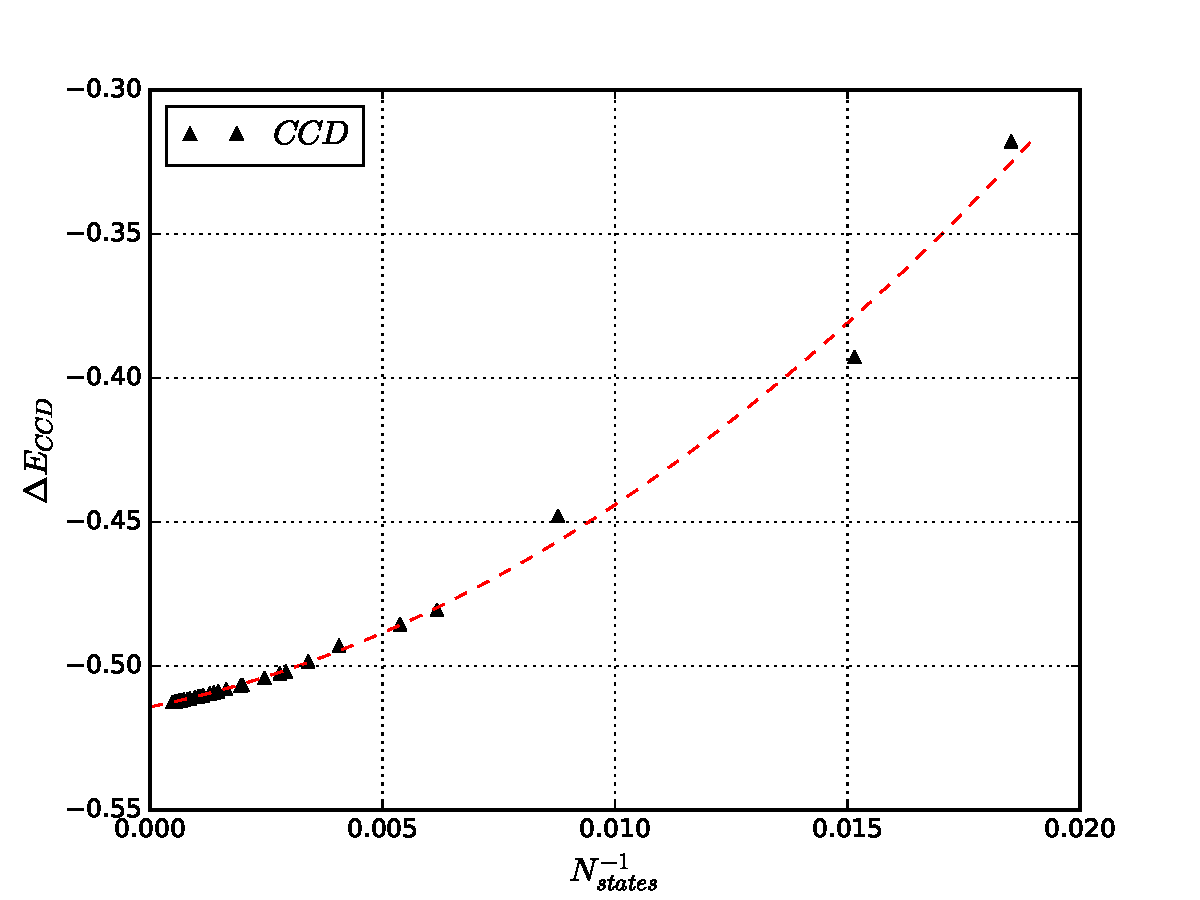
\includegraphics[width=0.8\linewidth]{cbs}
	\caption{The CBS limit for the 3D electron gas is extrapolated by a polynomial of degree two in $N_{states}^{-1}$. $N_{states}$ denotes maximum number os single-particle states included in basis. Calculations were performed for 14 electrons. We used Miller's\cite{MillerQuantumMechanicalStudies2017} results for higher number of states([406 - 2090]). Extracted limit for $N_{states} \rightarrow \infty$ was found to be -0.514204128446.}
	\label{fig:CBS}
\end{figure}






\section{CCQMC population dynamics}

While the electron gas is a common test system for deterministic many-body algorithms, its role as a proving ground for the CCQMC method should be considered with caution.
\begin{figure}[ht!]
	\centering
	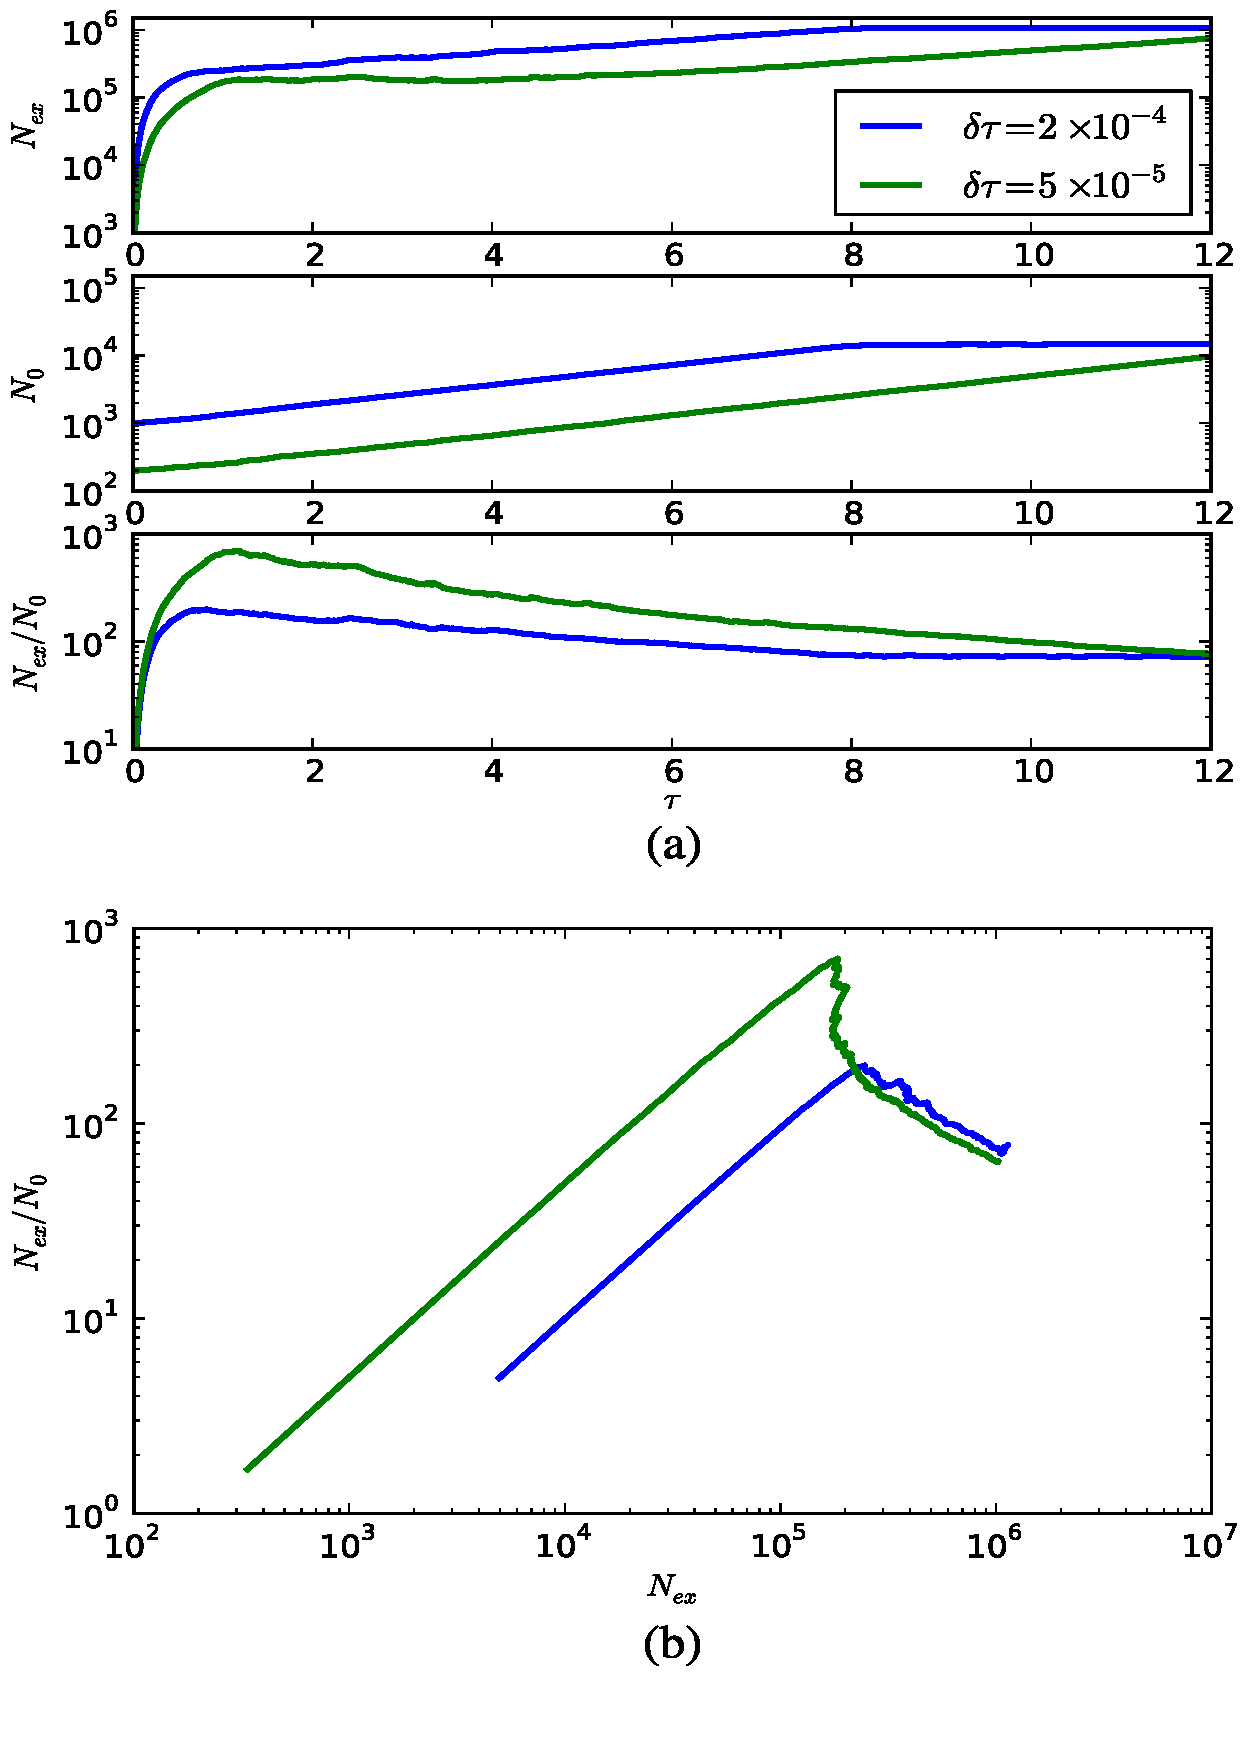
\includegraphics[width=0.8\linewidth]{thomEG}
	\caption{Ne cc-pVQZ CCSDTQ calculations starting with different initial
		particle numbers at the reference and different timesteps. (a): With a carefully
		chosen low timestep and initial population, a plateau is visible. An increased
		timestep and initial population overshoot the plateau but have a shoulder.
		The lower panel shows a maximum of the particle ratio at the position of
		the shoulder and plateau. (b): "Shoulder plots" allow shoulder height to be
		read off easily and calculations compared. Reproduced from \cite{SpencerDevelopmentsstochasticcoupled2016}, with the permission of AIP Publishing. }
	\label{fig:thomEG}
\end{figure}



The absence of singles, which is an indisputable advantage for deterministic methods, presents some difficulties for the stochastic coupled cluster. We try to examine these difficulties by analyzing sampling of all cluster sizes.

\begin{equation}\label{samplingsize}
   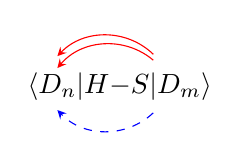
\begin{tikzpicture}[>=stealth,baseline,anchor=base,inner sep=0pt]
   \matrix (foil) [matrix of math nodes,nodes={minimum height=0.5em}] {
   	\langle & D_n & \mid & H & - & S & \mid & D_m & \rangle \\
   };
   \path[->] ($(foil-1-7.north)+(0,1ex)$)   edge[red,bend left=-45]  ($(foil-1-2.north)+(0,0.5ex)$);
   \path[->] ($(foil-1-7.north)+(0,1.5ex)$)   edge[red,bend left=-45]  ($(foil-1-2.north)+(0,1.5ex)$);
   \path[->, dashed] ($(foil-1-7.south)-(0,1ex)$)   edge[blue,bend left=45]  ($(foil-1-2.south)-(0,1ex)$);

   \end{tikzpicture}
\end{equation}

Foremost, we sample cluster of size zero, which corresponds the case when $\ket{D_m}$ is equal to the reference in (\ref{samplingsize}). We denote the level of excitation with red lines for the double and blue dashed line for the single excitation in (\ref{samplingsize}). For the electron gas we can choose only double excitation and spawn an excip on the double-excited determinant. There is no death of excips at cluster of size zero before the tunning of parameter $S$. That is, before annihilation plateau this sampling step produces only spawning events. And since we choose cluster size according to the exponential distribution, the reference is sampled $N_{ex}/2$ times, where $N_{ex}$ is the total population of excips.

Furthermore clusters of size one are sampled, where we can choose as $\ket{D_m}$ double- triple-excited determinant etc. Again, the bra-part should be single or double excitation of $\ket{D_m}$. Given that we refuse to choose singles, there is no spawning events for this cluster size. Only death events can occur in this case.
The number of samples is $N_{ex}/4$, which is two times less than the one for the reference. Hence possible outcome for death events is lower than for the spawn events from the cluster of size one. 


Lastly, we consider the clusters of size two. If we now turn to an atomic or a molecular system, we can construct a cluster of size two by picking a single excitation and then adding another single or double to it. Cluster, constructed from two singles, provides a death opportunity within CCSD truncation. Moreover, it also can initiate a spawning event(blue dashed line in (\ref{samplingsize})). 
The electron gas differs from systems with single excitations in the way that described mechanism of spawning/death is impossible. Within CCSD approximation the only possible form of these composite clusters is double + double. This results into quadruply-excited determinant in the ket part and double-excited determinant in the bra part. Quadruples participate in death process can be ignored within CCSD. Summing up the last arguments it is obvious that clusters of size two are source of spawning events only.


%Being Cautious 15


Critical population is needed  - plateau, different for systems, basis sets. Requires additional investigation.
Finding search for the annihilation plateu is critical part of ccqmc. spenser and thom claim that with 


It has been demonstrated that careful selection of simulation parameters might help to find annihilation plateau by eye \cite{SpencerDevelopmentsstochasticcoupled2016}. Spencer and Thom demonstrated that plateau is easy to see (figure \ref{fig:thomEG}(a)) for small values of $\tau$. However, these results were based upon data for the neon atom within CCSDTQ truncation. As it has been already discussed, every cluster size within such truncation results in death/spawn events. To verify the correctness of our implementation we need to obtain similar dynamics evolution in imaginary-time.
The most difficult parts of the CCQMC algorithm are the variation of the population on reference $N_0$ and the certainty of the sign structure. Since excips on reference are particles of another kind, it was decided that the best method to test sign structure was to fix population on reference and investigate population dynamics of the excited space only. We were unable to find in literature similar plots for the CCD truncation of the electron gas. We expected that behavior of the population of the excited space($N_{ex}$) should follow the pattern observed on figure \ref{fig:thomEG}(a). Figure \ref{fig:nx2k} presents dependence of $N_{ex}$ on $\tau$ for 14 electrons and 54 single-particle states. Earlier studies of the electron gas with the CCQMC method reported that for $r_s = 1$ and CCSDT the critical populations ranges from $10^4$ to $10^5$ \footnote{Estimation was obtained by the visual inspection of figure 8 in \cite{SpencerDevelopmentsstochasticcoupled2016}} for basis sizes from 203 to 2109 single particle states. Besides it was outlined that for the smaller values of $r_s=0.5$ the sufficient number of excips decreases to the value of roughly $10^3$ \footnote{within the CCSDT truncation for the 3D electron gas}. The current state of knowledge fails to establish correlations between the critical number of excips and the number of the basis state functions together with the level of correlation inside studied system. As it can be seen on figure \ref{fig:CCDvsCCDT}, the difference in the correlation energies for CCD and CCDT truncations decreases on decreasing $r_s$. Based on this we expected that the plateau height for $r_s=0.5$ should be near $10^3$ excips. Our estimations are presented on figure \ref{fig:nx2k}.

\begin{figure}[ht!]
	\centering
	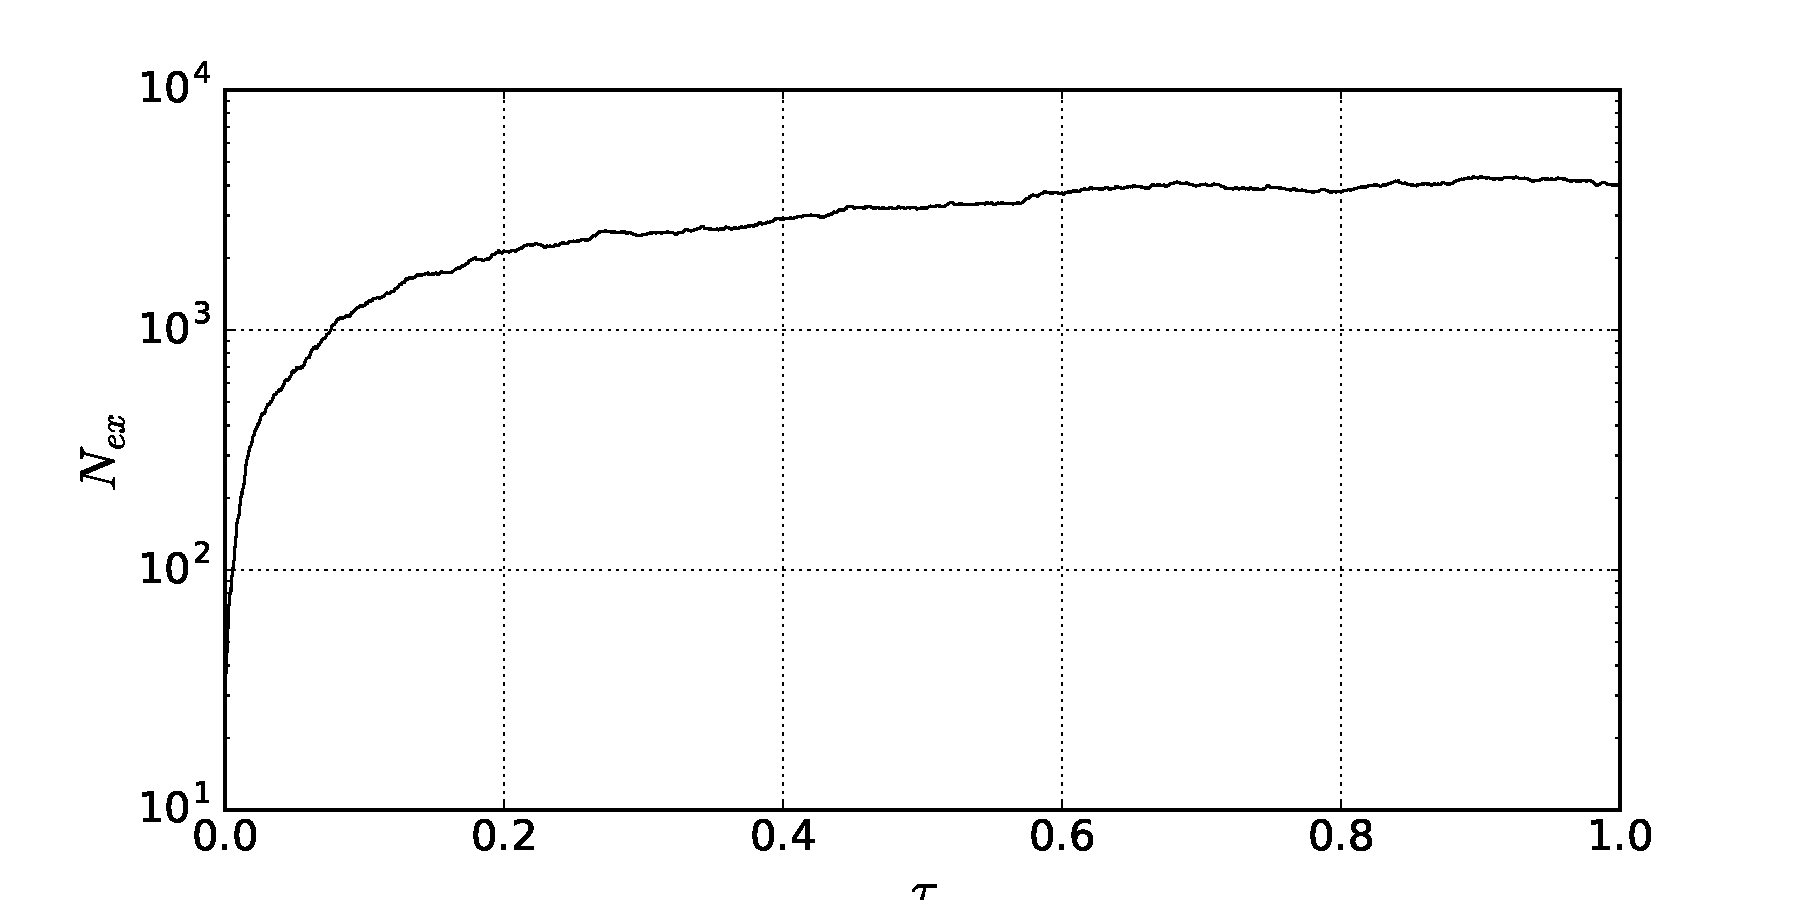
\includegraphics[width=0.8\linewidth]{Nex2000new}
	\caption{14 electrons rs 0.5 without tunning S etc tau 0.0005 2000 iter }
	\label{fig:nx2k}
\end{figure}
We tested same code for 162 basis state functions and observed same pattern, but with number of excips grown closer to $10^4$. These results would seem to suggest that the sign structure of the wave-function is correct.
However, these results should be treated cautiously since population on the reference was fixed in the beginning of the simulation. Additionally it can be seen from figure \ref{fig:platFind} that after 1600 iteration (that corresponds to the value of $\tau=0.6$ on figure \ref{fig:nx2k}) number of death and spawn events fluctuates around some value. That can mean that spawn and death probably give equal amount of positive and negative excips.

	
	



\begin{figure}[ht!]
	\centering
	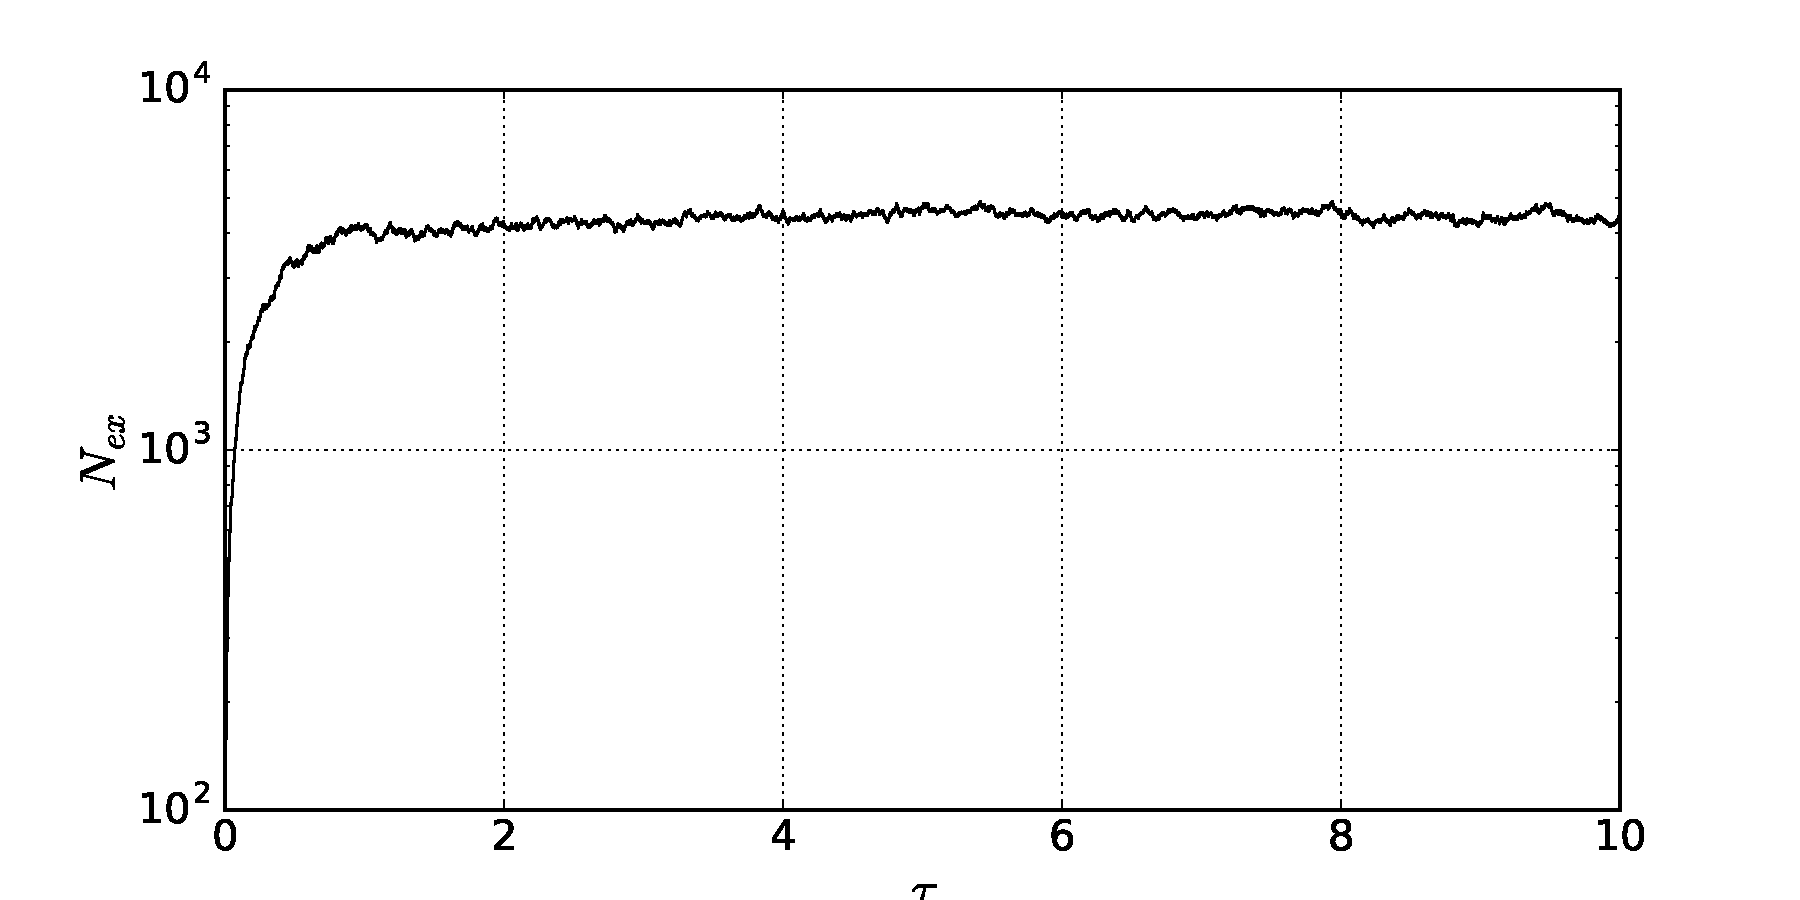
\includegraphics[width=0.8\linewidth]{Nex20000}
	\caption{14 electrons rs 0.5 with tunning S etc tau 0.0005 20000 iters}
	\label{fig:nx20k}
\end{figure}


\begin{figure}[ht!]
	\centering
	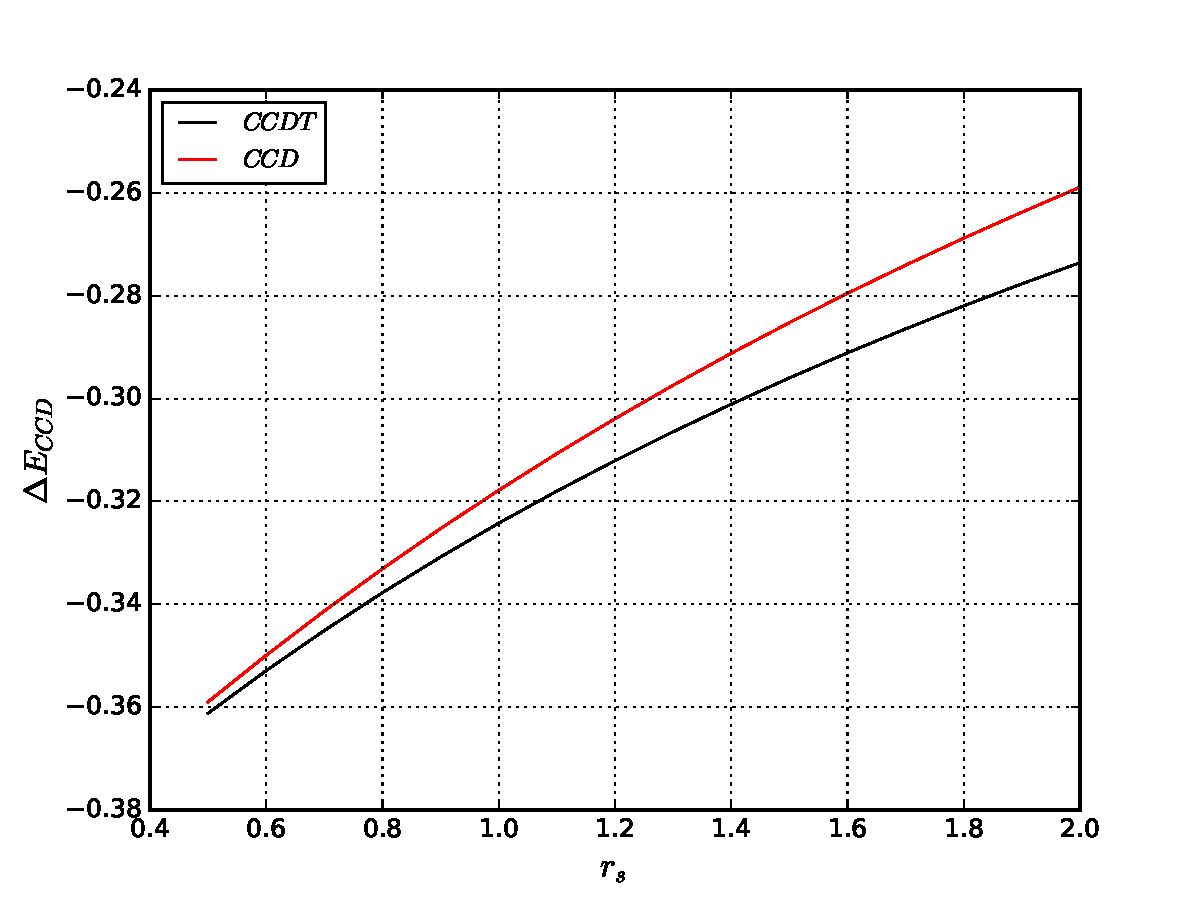
\includegraphics[width=0.8\linewidth]{CCDvsCCDT}
	\caption{14 electrons diff rs vs hansen}
	\label{fig:CCDvsCCDT}
\end{figure}



\begin{landscape}

\begin{figure}[ht!]
	\centering
	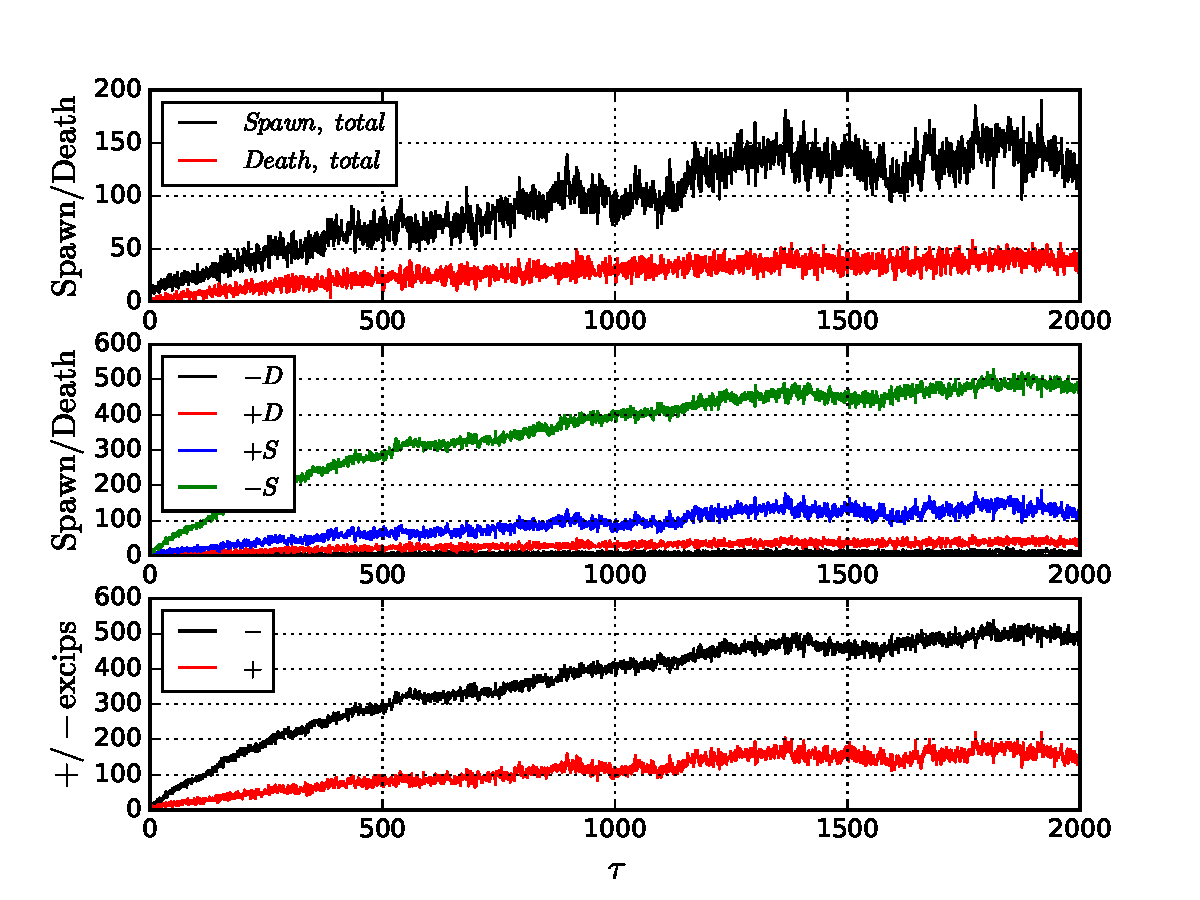
\includegraphics[width=0.8\linewidth]{platFind}
	\caption{14 electrons rs 0.5 without tunning S etc }
	\label{fig:platFind}
\end{figure}

\end{landscape}

\begin{landscape}
	
	\begin{figure}[ht!]
		\centering
		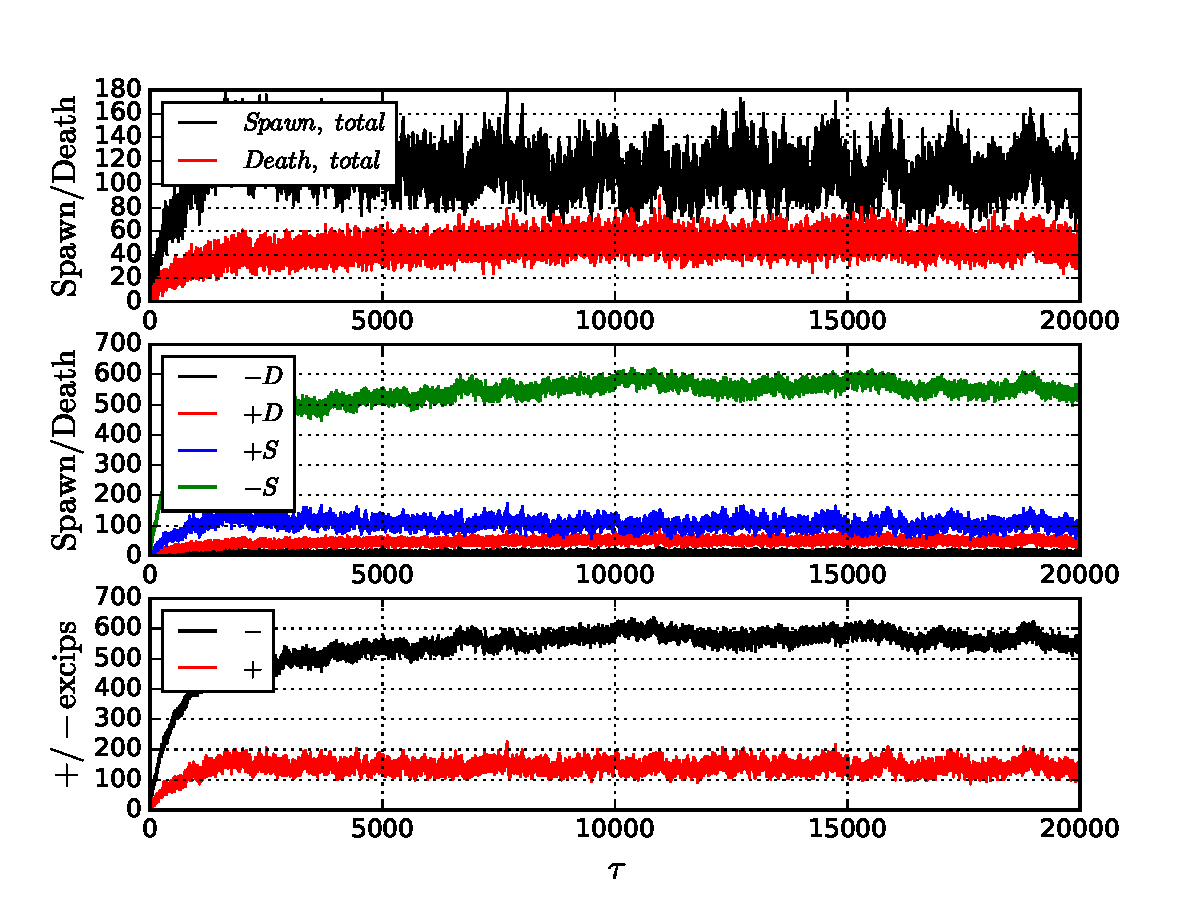
\includegraphics[width=0.8\linewidth]{platFindStune}
		\caption{14 electrons rs 0.5 with tunning S etc }
		\label{fig:platFindStune}
	\end{figure}
	
\end{landscape}






Proposed results

Small basis sets



\section{Conclusions And Future Prospects}

The method is quite new but seems to be a very promising one. There is still lack of the strict teory on convergence 

there are some studies on optimisation of the sampling schemes
At the moment of writing this thesis the only available results published were less than one year old


\appendix
\renewcommand{\thesection}{\Alph{section}.\arabic{section}}
\setcounter{section}{0}

\begin{appendices}
	
\section{Second quantization}
Creation operator is defined as follows:
\begin{equation}
c_p^\dagger\ket{\phi_q  \dots \phi_s}=\ket{\phi_p \phi_q  \dots \phi_s}.    
\end{equation}
If orbital $\phi_q$ already exists, the action of this operator results in zero:
\begin{equation}
c_p^\dagger\ket{\phi_p \phi_q  \dots \phi_s}=0.    
\end{equation}
Annihilation operator is defined as hermitian adjoint to the creation operator:
\begin{equation}
c_p\ket{\phi_p \phi_q  \dots \phi_s} = \ket{\phi_q  \dots \phi_s},
\end{equation}
where we have removed the first column and row from the Slater determinant. The action of the annihilation operator $c_p$ on a determinant without $\phi_p$ orbital will result into zero: 
\begin{equation}
c_p\ket{\cancel{\phi_p} \phi_q  \dots \phi_s} = 0.
\end{equation}
The zero particle space is defined as a one-dimensional space spanned by the special state, called the $vacuum\  state$ $\ket{-}$. It's worse mentioning that the vacuum state is not zero. Thus a string of the creation/annihilation operators, acting on the vacuum can create a Slater determinant:
\begin{equation}
c_1^\dagger \dots c_N^\dagger \ket{-} = \ket{\phi_1 \dots \phi_N}.
\end{equation}

Pairwise permutations of the operators change the sign of the resulting determinant. It is easy to see on the example with two orbitals:
\begin{equation}
c_q^\dagger c_p^\dagger \ket{-} = \ket{\phi_q \phi_p} = - \ket{\phi_q \phi_p} = - c_p^\dagger c_q^\dagger  \ket{-}.
\end{equation}
The following properties can be derived for the relation of general creation/annihilation operators:
\begin{align}
\begin{split}
\{c_p, c_q\} = 0,\\
\{c_p^\dagger, c_q^\dagger\} = 0,\\
\{c_p, c_q^\dagger\} = \delta_{p,q}.
\end{split}
\end{align}

\section{Particle-hole formalism}
It is more convenient to work with $n$-electron reference(vacuum) determinant than with true vacuum $\ket{-}$. Reference vacuum is often called $Fermi\ vacuum$.

We divide all single-particle functions into two subsets. The first subset corresponds to the occupied single-particle states and denoted by indices $i,j,k\dots$. The second contains all unoccupied (also called $virtual$) single-particle states. We reserve indices $a,b,c \dots$ for these states. Single-particle states which are occupied in the reference determinant($i,j,k\dots$) are called $hole$ states. Similarly, unoccupied states( $a,b,c \dots$) are referred to as $particle$ states. 
Annihilation operator $\hat{c}_i$ destroys particle located on the occupied orbital $i$, or with other words, creates a hole state. So $\hat{c}_i$ can be considered as a quasi-particle(hole) creation operator. Similar trail of thoughts can be introduced for the $\hat{c}^\dagger$ operator. Thus, we define quasi-particle annihilation operators as those that annihilate holes and particles: $c_i^\dagger$ and $c_a$. Similarly, quasi-particle creation operators are introduced: $c_i$ and $c_a^\dagger$. Anticommutator relations are changed for these quasi-particle operators, and the only non-zero ones are:
\begin{align}
\begin{split}
\{c_i^\dagger c_j\} = \delta_{ij},\\
\{ c_a c_b^\dagger\} = \delta_{ab}.
\end{split}
\end{align} 


\section{Normal ordering}

If one considers a string of second-quantization operators(for example, creation/annihilation), this string is referred to as $normal-ordered$ if all annihilation operators stand to the right of all creation
operators. It is usually denoted by $\{\}_N$. Subscript $N$ is often omitted.
\begin{equation*}
\text{Normal orderes string} = \text{(creation operators)} \cdot \text{(annihilation operators)}.
\end{equation*}
More strictly we can write:
\begin{equation}
\{A_1 A_2 \dots A_n\} = (-1)^{\sigma} \text{normal orderes string},
\end{equation}
where $\sigma$ is a number of permutations needed to rearrange the operators such, that their product is written on the normal ordered form.
This form of writing of the operator strings is extremely useful, since the action of such string on the vacuum state is always zero by the definition of the annihilation operator. The latter is true both for the true vacuum and for the Fermi vacuum.

\section{Wick's theorem}
To formulate Wick's theorem some definitions are needed.

Contraction between two arbitrary creation and annihilation operators is denoted by:
\begin{equation*}
\wick{\c1 X \c1 Y},
\end{equation*}
and represents the difference between current given order and a normal order:
\begin{equation}
\wick{\c1 X \c1 Y}= XY - \{XY\}.
\end{equation}
There is only one non-zero contraction between a pair of the creation and the annihilation operators:
\begin{equation}
\wick{\c1 c_p \c1 c_q^\dagger} = c_p c_q^\dagger -  \{c_p c_q^\dagger\}=\delta_{pq}.
\end{equation}

Contraction inside the operator string.\\
Let $A_1 A_2 \dots A_n $ be an product of arbitrary second-quantized operators. We choose $A_q$ and $A_p$ to be a pair of the operators, and denote number of possible permutation which places $A_q$ to the first place and $A_p$ to the second place as $\sigma$.
\begin{equation}
\wick{\{ A_1 \dots \c1 A_q  \dots \c1 A_p \dots A_n \} } = (-1)^{\mid \sigma \mid} \wick{ \{  \c1 A_q  \c1 A_p A_{\sigma(3)} \dots A_{\sigma(n)} \} }.
\end{equation}
where $\sigma$ is any number of permutations, satisfying $\sigma(1)=q$ and $\sigma(2)=p$.		


\subsubsection{Wick's theorem}
Any operator string of creation and annihilation operators can be written as its normal ordered form plus a sum of all possible contractions inside normal ordered form.\\
\begin{align}\label{WICK}
\begin{split}
A_1 A_2 \dots A_n=\{A_1 A_2 \dots A_n\} + \sum_{\substack{\text{all single} \\ \text{contractins}}} \underbrace{ \{ \wick{\c1 A_1 A_2 \c1 \dots A_n}\} }_{\substack{\text{all single-} \\ \text{contracted terms}}} +\\ \sum_{\substack{\text{all double} \\ \text{contractins}}} \underbrace{ \{ \wick{ \c1 A_1 \c2 A_2 \c2 \dots \c1 A_n}\} }_{\substack{\text{all double-} \\ \text{contracted terms}}}+ \dots +
\sum_{\substack{\text{all $\frac{n}{2}$} \\ \text{contractins}}} \underbrace{ \{ \wick{ \c1 A_1  \c2 A_2 \c3 \dots \c2 \dots \c1 \dots \c3 A_n }\} }_{\substack{\text{all $\frac{n}{2}$-} \\ \text{contracted terms}}}.
\end{split}
\end{align}
If $n$ is odd, all terms in the last sum of equation (\ref{WICK}) have one uncontracted operator. 

\subsubsection{Generalized Wick's theorem}
Generalization of Wick's theorem extends it application to the case of multiple products of normal ordered substrings. Let us consider substring product:
\begin{equation*}
\Lambda = \{ A_1 A_2 \dots  A_n \}\{ B_1 B_2 \dots  B_n \} \dots \{ Z_1 Z_2 \dots  Z_n \}.
\end{equation*}
Then $\Lambda$ can be written as a sum over all fully-contracted sets of normal-ordered substrings:
\begin{align}\label{WICKGen}
\begin{split}
\Lambda = \{ A_1 A_2 \dots  A_n \vdots B_1 B_2 \dots  B_n \vdots \dots \vdots Z_1 Z_2 \dots  Z_n \} +\\
 \sum_{\substack{\text{all single} \\ \text{contractins}}} \underbrace{ \{ \wick{\c1 A_1 A_2 \dots  A_n \vdots B_1 B_2 \dots  B_n \vdots \dots \vdots Z_1 \c1  Z_2 \dots  Z_n}\} }_{\substack{\text{all single-} \\ \text{contracted substrings}}} + \\
\dots + \\
 \sum_{\substack{\text{all $\frac{n}{2}$} \\ \text{contractins}}} \underbrace{ \{ \wick{ \c1 A_1 \c2 A_2 \dots \c3 A_n \vdots \c4 B_1 \c1 B_2 \c5 \dots \c6 B_n \vdots \dots \c2 \dots \vdots \c5 Z_1 \c6 Z_2 \c3 \dots  \c4 Z_n }\} }_{\substack{\text{all $\frac{n}{2}$-} \\ \text{contracted substrings}}}.
\end{split}
\end{align}



%	\subsection{foo title}
%	\[
%	f^{p}_{q} \left\{a^\dagger_{p} a_{q}\right\} - \frac{v^{pq}_{rs}}{4} \left\{a^\dagger_{p} a^\dagger_{q} a_{r} a_{s}\right\}
%	\]
%	CC Energy:
%	\[
%	f^{k}_{c} t^{c}_{k} - \frac{t^{c}_{l} t^{d}_{k}}{2} v^{kl}_{cd} + \frac{t^{cd}_{kl} v^{kl}_{cd}}{4}
%	\]
%	CC T1:
%	\begin{gather*}
%	- f^{k}_{c} t^{c}_{i} t^{a}_{k} + f^{k}_{c} t^{ac}_{ik} - f^{k}_{i} t^{a}_{k} + f^{a}_{c} t^{c}_{i} + f^{a}_{i} - t^{c}_{k} t^{d}_{i} t^{a}_{l} v^{kl}_{cd} - t^{c}_{k} t^{d}_{i} v^{ak}_{cd} + t^{c}_{k} t^{a}_{l} v^{kl}_{ic} +\\
%	t^{c}_{k} t^{ad}_{il} v^{kl}_{cd} + t^{c}_{k} v^{ak}_{ic} - \frac{t^{c}_{i} t^{ad}_{kl}}{2} v^{kl}_{cd} + \frac{t^{a}_{l} t^{cd}_{ik}}{2} v^{kl}_{cd} + \frac{t^{cd}_{ik} v^{ak}_{cd}}{2} - \frac{t^{ac}_{kl} v^{kl}_{ic}}{2}
%	\end{gather*}
%	CC T2:
%	\begin{gather*}
%	f^{k}_{c} t^{c}_{i} t^{ab}_{jk} P(ij) - f^{k}_{c} t^{a}_{k} t^{bc}_{ji} P(ab) + f^{k}_{i} t^{ab}_{jk} P(ij) + f^{a}_{c} t^{bc}_{ji} P(ab) + t^{c}_{k} t^{d}_{i} t^{ab}_{jl} v^{kl}_{cd} P(ij) - t^{c}_{k} t^{a}_{l} t^{bd}_{ji} v^{kl}_{cd} P(ab) +\\ t^{c}_{k} t^{ad}_{ji} v^{bk}_{cd} P(ab) + t^{c}_{k} t^{ab}_{il} v^{kl}_{jc} P(ij) + t^{c}_{i} t^{d}_{j} t^{a}_{k} t^{b}_{l} v^{kl}_{cd} + t^{c}_{i} t^{d}_{j} t^{a}_{k} v^{bk}_{cd} P(ab) + \frac{t^{c}_{i} t^{d}_{j}}{2} t^{ab}_{kl} v^{kl}_{cd} +\\ t^{c}_{i} t^{d}_{j} v^{ab}_{cd} - t^{c}_{i} t^{a}_{k} t^{b}_{l} v^{kl}_{jc} P(ij) - t^{c}_{i} t^{a}_{k} t^{bd}_{jl} v^{kl}_{cd} P(ab) P(ij) - t^{c}_{i} t^{a}_{k} v^{bk}_{jc} P(ab) P(ij) - t^{c}_{i} t^{ad}_{jk} v^{bk}_{cd} P(ab) P(ij) -\\ \frac{t^{c}_{i} t^{ab}_{kl}}{2} v^{kl}_{jc} P(ij) - t^{c}_{i} v^{ab}_{jc} P(ij) - \frac{t^{a}_{k} t^{b}_{l}}{2} t^{cd}_{ji} v^{kl}_{cd} - t^{a}_{k} t^{b}_{l} v^{kl}_{ji} - \frac{t^{a}_{k} t^{cd}_{ji}}{2} v^{bk}_{cd} P(ab) + t^{a}_{k} t^{bc}_{il} v^{kl}_{jc} P(ab) P(ij) -\\ t^{a}_{k} v^{bk}_{ji} P(ab) + \frac{t^{cd}_{jk} t^{ab}_{il}}{2} v^{kl}_{cd} P(ij) - \frac{t^{cd}_{ji} t^{ab}_{kl}}{4} v^{kl}_{cd} - \frac{t^{cd}_{ji} v^{ab}_{cd}}{2} + t^{ac}_{ik} v^{bk}_{jc} P(ab) P(ij) \\- t^{ac}_{jk} t^{bd}_{il} v^{kl}_{cd} P(ab) + \frac{t^{ac}_{ji} t^{bd}_{kl}}{2} v^{kl}_{cd} P(ab) - \frac{t^{ab}_{kl} v^{kl}_{ji}}{2} - v^{ab}_{ji}
%	\end{gather*}
	
\end{appendices}



\printbibliography



\end{document}
